\documentclass[master]{thesis-uestc}

\renewcommand\labelenumi{(\theenumi)}

\title
{基于图网络的广域网路由异常检测研究}
{Wide Area Networks Routing Anomaly Detection based on Graph Networks}

\author{杨畅}{Yang Chang}
\advisor{邵俊明\chinesespace 教授}{Dr. Shao Junming}
\school{计算机科学与工程学院}{School of Computer Science and Engineering}
\major{计算机科学与技术}{Computer Science and Technology}
\studentnumber{202021081817}

% require all the usepackages here
% \usepackage{algorithm2e}

\begin{document}

\makecover

\originalitydeclaration

% abstract

\begin{chineseabstract}
    随着互联网络产业的快速发展,广域网作为网络核心基础设施,在协议和规模层面不断拓展,同时也带来了诸多问题和挑战。广域网络中的路由异常,由于其隐蔽、复杂和无法根除的特点,成为了近年来通信和计算机领域中一个值得深入研究的问题。为了在真实网络环境中及早检测并过滤这一类异常路由,以防止其通过路由系统扩散至全球并对网络系统产生危害,对路由更新条目进行嵌入并进一步进行异常检测是很有必要的。迄今为止,大多现已提出的算法和应用于工业中的模型还尚在使用基于时间序列分析的方式研究此问题的阶段,而选择此种研究方法意味着模型将在质量、数量、特征三个方面存在问题。首先,现有的广域网络路由数据集在数量上能够满足一般异常检测任务模型训练的要求,但这些数据并非针对图网络而设计,存在冗余数据过多、具有无效连边和路径的问题,进而影响基于图网络的异常检测算法的性能。其次,针对现有规模庞大的网络路由数据集,传统的卷积网络因其复杂度过高的原因,运算能力和效率成为了一项难以解决的问题。最后,放弃数据集中的几乎全部拓扑信息,使得学习到的模型在泛化性上存在不足,很难被使用于各种结构关系并不相同的分布式网络中。

    \begin{enumerate}
        \item 针对现有网络数据集存在的冗余和无效数据问题,本文基于网络的路径选择和图网络相似度两种度量提出了两种图网络构建算法,实现对路由数据的精准网络建模,并降低图的复杂性和稠密度。在与不同基线模型的对比实验中,数据集在图网络下的性能提升得到了有效验证。
        \item 针对图卷积网络无法处理大尺度数据集的问题,本文基于GraphSAGE 算法的聚合模型提出了新的以路径特征为权重的采样方式、聚合和损失函数,从而构造出一种基于路径信息聚合的异常检测模型,实现对邻居特征及路径信息的聚合,提高了异常检测的效率和性能。在互联网和分布式网络数据集的对比和消融实验中,多项指标证明了此模型的有效性。
        \item 针对数据集中随机路径采样特征的利用方法问题,本文基于随机游走分析了路由路径的特点,提出了一种对路由数据进行针对性采样的方法,据此实现了更加高效鲁棒的检测模型,降低了问题的复杂性,摆脱了以路径为单元的异常检测任务对完整构图的依赖。在多个网络数据集上的多种任务结果表明模型的异常效果在大部分场景下优于其它基线方法。
    \end{enumerate}
    \chinesekeyword{异常检测;图嵌入;图网络}
\end{chineseabstract}



\begin{englishabstract}
    With the rapid development of the interconnection network industry, wide area networks, which are the core infrastructure of networks, are in the process of continuous expansion at the protocol and scale levels, and bring many problems and challenges along with the rapid development of technology. Routing anomalies in wide area networks have become a problem worthy of in-depth study in the field of communication and computing in recent years due to their hidden, complex and uneradicable characteristics. In order to detect and filter this class of anomalous routes early in real network environments to prevent them from spreading globally through the routing system and causing harm to the network system, it is necessary to embed and further anomaly detection for routing update entries. So far, most of the algorithms that have been proposed and models applied in industry are still at the stage of studying this problem using a time-series analysis-based approach, and the choice of such a research method implies that the models will have problems in three aspects: quality, quantity, and characteristics. First, the existing wide-area network routing datasets are quantitatively sufficient for training models for general anomaly detection tasks, but they are not designed for graph networks and suffer from excessive redundancy, invalid connected edges and paths, which affect the performance of graph network-based anomaly detection algorithms. Second, for the existing large scale network routing dataset, the traditional convolutional network becomes an intractable problem in terms of computing power and efficiency due to its excessive complexity. Finally, giving up almost all the topological information in the dataset makes the learned model inadequate in generalization and difficult to be used in various distributed networks with different structural relationships.

    \begin{enumerate}
        \item To address the problem of redundant and invalid data in existing network datasets, this paper proposes two graph network construction algorithms based on two measures of path selection and graph network similarity of networks to achieve accurate network modeling of routing data and reduce the complexity and density of graphs. In the comparison experiments with different baseline models, the performance improvement of the dataset under graph networks is effectively verified.
        \item To address the problem that graph convolutional networks cannot handle large scale datasets, this paper proposes a new sampling method, aggregation and loss function based on the aggregation model of GraphSAGE algorithm with the weight of path features, thus constructing an anomaly detection model based on the aggregation of path information to realize the aggregation of neighbor features and path information, which improves the efficiency and performance of anomaly detection. In the comparison and ablation experiments of Internet and distributed network datasets, several metrics prove the effectiveness of this model.
        \item To address the problem of utilizing random path sampling features in datasets, this paper analyzes the characteristics of routing paths based on random wandering, and proposes a method for targeted sampling of routing data, whereby a more efficient and robust detection model is implemented, reducing the complexity of the problem and freeing the path-based anomaly detection task from the dependence on complete composition. The results of multiple tasks on multiple network datasets show that the anomaly effect of the model outperforms other baseline methods in most scenarios.
    \end{enumerate}
    \englishkeyword{Anomaly Detection;Graph Embedding;Graph Network}
\end{englishabstract}

\thesistableofcontents

\chapter{绪\hspace{6pt}论}

% 10-12.5 页

\section{研究工作的背景与意义}

% 3 页

互联网(Internet)是人类信息社会的标志性基础设施之一,它的出现不仅改变了人们的生活方式,也改变了人类社会的发展趋势。从一开始的电脑与电脑之间直接互相作为对等体(Peer)连接交换路由和数据,到互联网的商业化,使得能够较大范围提供互联网服务的服务器、交换机、路由器等专用设备的出现,再到近十年来云计算、物联网、大数据和分布式的人工智能系统概念兴起的背景下,互联网络的规模和复杂度日益增加。一些互联网的调研项目共同指出,广域网络(Wide Area Network)作为跨越全球各个国家和地区将若干数据中心、接入网和终端设备彼此连接的全球计算机系统,已然成为不同地域、组织和用户跨越空间限制进行信息获取和交流的主要手段\citing{douzet2020measuring} \citing{oliveira2009completeness}。它为网络带来了层次性,一定程度上简化了网络的架构,方便了网络服务商、运营商,推动了更大规模的网络发展。

广域网络本质上是一个分布式的网络系统\citing{douzet2020measuring},由不同规模的成员网络相互连接,彼此交换数据。其中,在同一行政控制下的网络路由器组成的一组网络通常拥有相同或相似的路由表、路由选择策略和网络参数,这样的一组网络在广域网际路由协议\citing{rekhter2006border}中被称为自治系统(Autonomous System,AS),是互联网中广域网的基本组成单元。这些自治系统被互联网资源管理机构赋予了唯一的自治系统号(ASN),用于在全球范围内标识和识别该自治系统。

除了最广泛被应用的互联网(同时也是目前最大的广域网络),不少社区组织和科研机构都会自发地组建不同于互联网的分布式网络,它们的管理方式和结构与互联网有着较大的差异:据现有资料显示,一些社区网络提供比互联网更加开放、灵活的连接方式\citing{tsai2022design},从而形成截然不同的拓扑结构。

网络数据的传输大多会以数据包的形式在网络上进行传输,在进入广域网的范畴后,它通常需要经过许多归属不同自治系统的路由器的中转才能抵达最终的目的地。这些路由器即是自治系统中路由功能的最小组成单元\citing{douzet2020measuring},它们在接受到数据包后,会根据内部的路由规则将其进行处理,并转发到下一个路由器\citing{aweya2001ip}。 在这个过程中,路由器之间需要通过一种或多种协议进行协作,以保证数据包能够以最快、最稳定的方式传输。

为了确定数据包传输的最佳路径,路由协议被用来进行路由选择。自治系统内的路由器通过内部路由协定(如 OSPF、IS-IS、Babel 等)共享路由信息,而不同自治系统之间的路由信息则通过边界网关协定(BGP)\citing{rekhter2006border}进行交换。 BGP 使用了许多因素来决定数据包的最佳路径,如最短自治系统路径、最低成本或是最可靠的链路等。BGP 协议的路由选择中最重要的指标是最短自治系统距离,它用于衡量从当前网络抵达目的自治系统的路线上,基于自治系统衡量的最短逻辑距离\citing{aweya2001ip}。这种路径选择方式无法达到物理距离的最优解,然而根据在实际网络传输业务的数据调研\citing{feamster2004model}中发现的结果,在政策和线路利用率约束下,逻辑上的最优方案能够有效地减少延迟和网络拥塞,从而提高网络的传输效率。

一种简化了的广域网流量路径如图 \ref{c1_wan-flow} 所示,位于自治系统 A 的终端设备发送数据包至位于自治系统 B 的终端设备,路由器 $A_i$,$B_j$ 分别为自治系统 A、B 的其中一对边界路由器。数据包在首次经过边界路由器后即进入广域网络的范畴,根据边界网关协定的路由规则被转发,直至第二次穿过边界路由器,进入自治系统 B 中,并通过内部网络抵达目标地址。

\begin{figure}[h]
    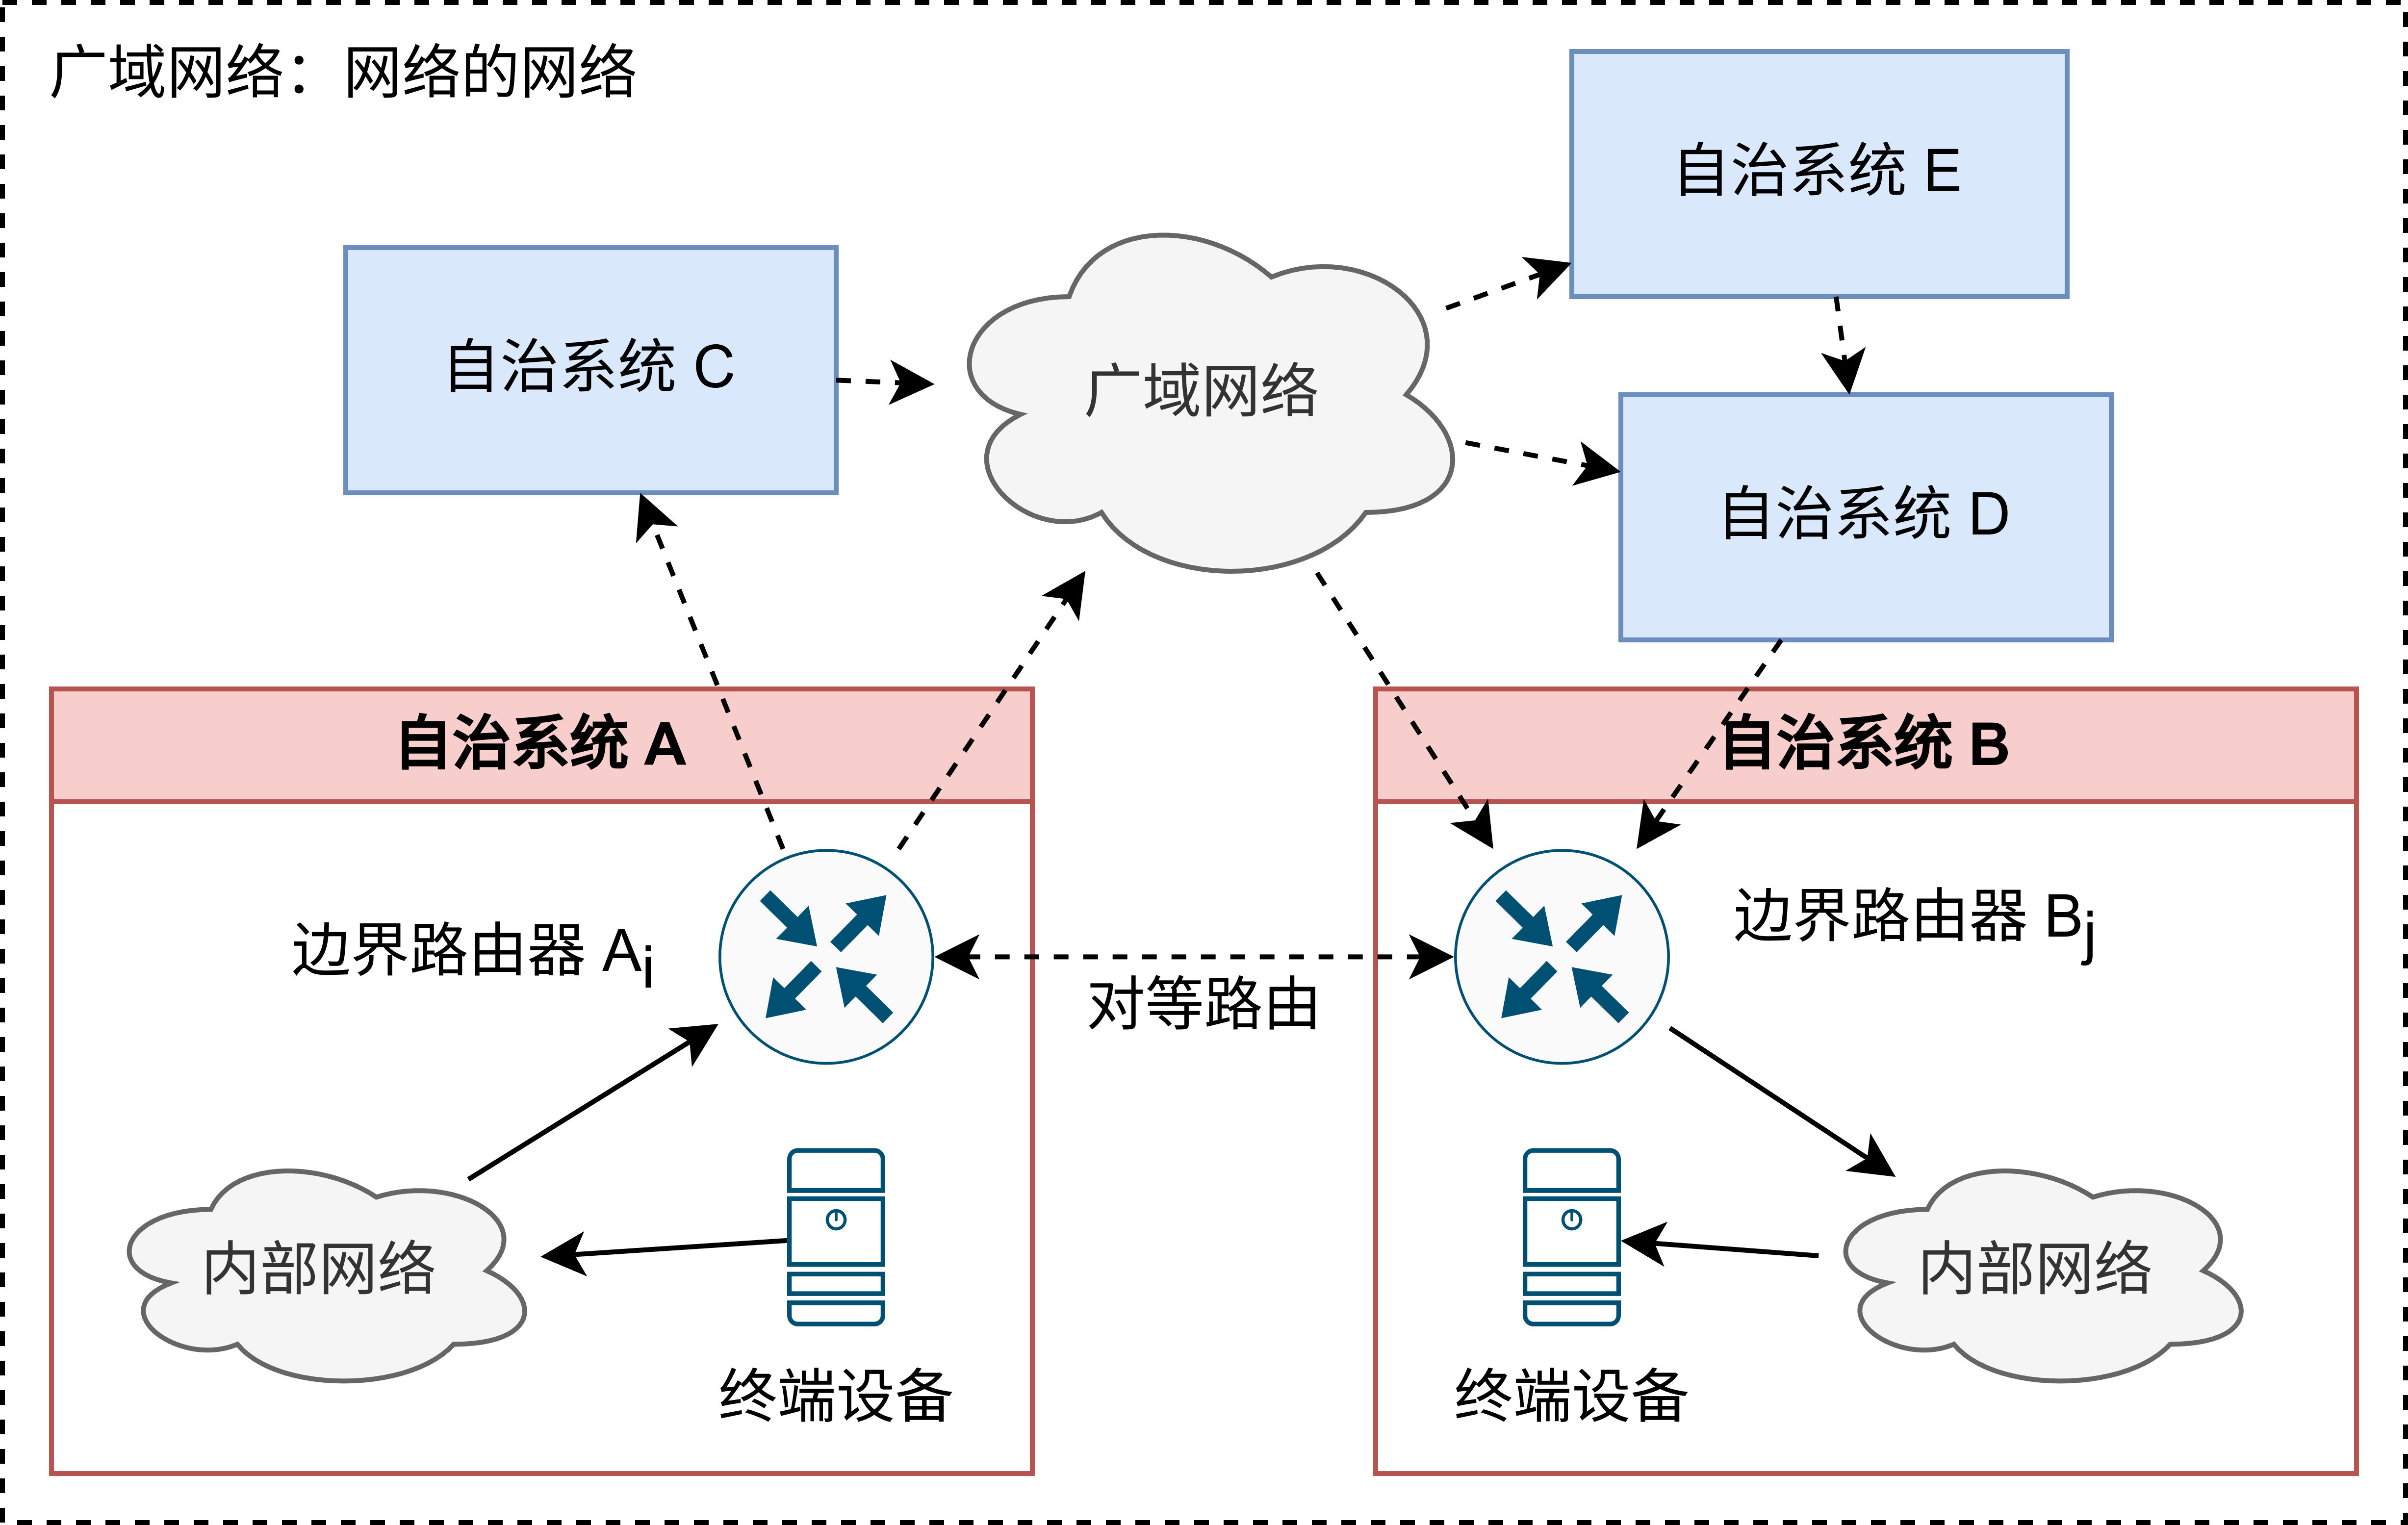
\includegraphics[width=0.7\linewidth]{chapter/c1_images/c1_wan-flow.png}
    \caption{流量途径局域与广域网络}
    \label{c1_wan-flow}
\end{figure}

在实际应用中,BGP 会通过 TCP/IP 协议相互交换并转递路由信息\citing{rekhter2006border},藉此了解其他自治系统之间的网络拓扑和路由策略,从而进行合理的路由选择。同时,由于路由表的开放性允许同一个网络被不同的运营商宣告为不同的路径,BGP 能够支持多路径路由\citing{feamster2004model},即在数据包传输过程中,可以选择多个路径进行传输,有研究指出此种路由方式提高了传输的可靠性和鲁棒性\citing{augustin2010measuring},也为提供全球性互联网服务提供了便利。 

然而,正是由于广域网结构的分布式和松散的特点,BGP 协议的核心机制中存在着一些固有的缺陷,例如在一项研究中总结的,其交换信息不受限制,而且没有强制的身份验证\citing{butler2009survey},使其在面对错误配置、异常行为或劫持攻击的情形下极为脆弱:BGP 路由信息能够在传递过程中任意修改,使得原本流向目的地的数据流量能够被不加验证地重定向到其它位置,在蓄意策划的异常情况下,能够使得攻击者不需要对目标网络系统做出任何改动即可截获和提取流量中的敏感信息。

BGP 路由异常对网络的影响也是全球性的,它可能会导致许多严重后果,如大规模的服务中断、网络可用性降低和网络失去信任等,最终影响整个广域网的连通性、稳定性和安全性,这引起了网络运营商和网络管理机构的重视,一些与网络安全相关的研究多次指出了这一点\citing{butler2009survey}。以下是几次具有代表性、影响较大的互联网路由异常的例子:

\begin{enumerate}
    \item 2008年,巴基斯坦的电信公司意外地劫持了互联网的很大一部分(包括谷歌、雅虎和其他主要网站)的流量。这是由一个配置错误的 BGP 路由器造成的,该路由器向互联网的其他部分公布了错误的路由信息\citing{ripe2008youtube}。
    \item 2010年,内容分发网络(CDN)供应商 Akamai 经历了一次BGP劫持,将本应到达其客户网络的流量被重定向到不同的地方\citing{hiran2013characterizing},导致服务中断和客户对网络失去信任。
    \item 2020年,一个BGP劫持事件影响了美国、欧洲和中东的互联网流量,将用于谷歌和亚马逊的流量重定向到不同的位置。这是由中国的一个错误配置的BGP路由器造成的\citing{graham2020cloudflare}。
    \item 2022年,一次BGP劫持被用来将加密货币交易所的流量重定向到不同的位置,使攻击者能够拦截敏感数据并窃取加密货币\citing{siddiqui2022klayswap}。此事故及其导致的严重损失引发了各界对广域网络路由安全的关注。
\end{enumerate}

在互联网的发展历程中,有很多用于缓解和避免路由异常的协议或方法被提出来,例如用于过滤无效路由的资源公钥基础设施(RPKI)标准 \citing{bush2013resource} 和用于降低路由更新频率、降低路由器负载的路由震荡抑制(Route Dampening)技术\citing{villamizar1998bgp}, 同时也有研究机构搭建公共的路由收集器\citing{orsini2016bgpstream},以此发布公开可用的数据集\citing{mao2003bgp},并提供基于不同指标的路由异常检测方案。

然而,上述方法并不能彻底解决广域网络中存在的安全性问题,也不足以应付复杂多变的网络环境。广域网络的策略、标准和局部拓扑结构在不同位置具有截然不同的特点,这是通过固定的度量标准难以实现的。近年以 FITI (国家未来互联网试验设施)\citing{谢高岗2012未来互联网体系结构研究综述}、DN42(42 号分布式网络)\citing{dn42us}为例的分布式网络实验系统的出现更是为现有模型的可迁移性提出了挑战\citing{tsai2022design}。

在广域网络路由中使用基于图的机器学习方法是具有一定依据的,路由协议本身即是一种图网络算法,一些路由指标能够很好地提供除图网络的拓扑结构以外的数据,同时,由于类似路由异常检测的带外程序无需直接与路由系统交互、不需要严格的收敛时间等响应要求,如何在路由异常检测上采用图网络模型是一种潜在的研究方向\citing{sanchez2019comparing}。

然而目前图模型在广域网的异常检测中应用并不广泛,由于广域网络的路由数据集的特征决定了它们无法直接在图网络模型中使用,一项调研指出当前的研究大多集中于中小型网络内部的局域网拓扑\citing{moustafa2019holistic}。

本研究将通过分析几类不同方向的图网络模型在不同规模的网络数据集上的检测效果,旨在探索图网络算法在路由异常检测中的应用,并据此构建出新颖高效的广域网路由异常检测模型,使其能够较好地利用网络路由中携带的拓扑信息。


\section{国内外研究历史与现状}

% 3-4 页

由于众多路由异常事件对生产造成的巨大损失,已有一些技术和研究针对此问题进行了探讨\citing{sermpezis2018survey}。当前国内外对路由异常问题的研究主要分为缓解方法和检测方法两种大致方向:缓解方法通过在路由器引入一些针对性的协议从而阻止异常路由在网络之间转发;检测方法旨在通过一系列的算法和模型从实时更新的路由表中检测存在风险的路由。

\subsection{基于信任数据库的路由异常缓解方法}

资源公钥基础设施(RPKI)\citing{bush2013resource}是一个使用数字证书和公钥基础设施(PKI)来验证互联网路由信息的系统。它试图从源头和标准上控制路由异常的发生,旨在通过允许网络运营商对其路由公告进行加密签名并验证从其他网络收到的路由信息的真实性,以达到阻止 BGP 异常路由的产生。

RPKI 试图在分布式的广域网路由系统中建立中心化的信任数据库,并通过层次化的信任关系传递授权数据,反映到实际操作中即为运营商掌握的数字签名及其对应的私钥。如图 \ref{c1_rpki} 所示,RPKI 体系的工作方式与现代通用的证书系统大体上保持一致,运营商通过私钥签署自己信任的路由信息,并通过同样的方式吊销已签发的授权信息,这些信息将以数字证书的形式上传至 PKI 系统储存,并通过证书吊销列表(CRL)\citing{al2012development}的方式更新。 路由器在工作时,将连接至 PKI,通过证书的签名和有效性验证接收到的路由信息的真实性,进而选择接受或是丢弃路由。证书机制具有数学上可形式化验证的安全性,因而运营商可以确保接收到的路由是合法的,从而从源头上防止 BGP 劫持的发生\citing{wahlisch2012towards}。

\begin{figure}[h]
    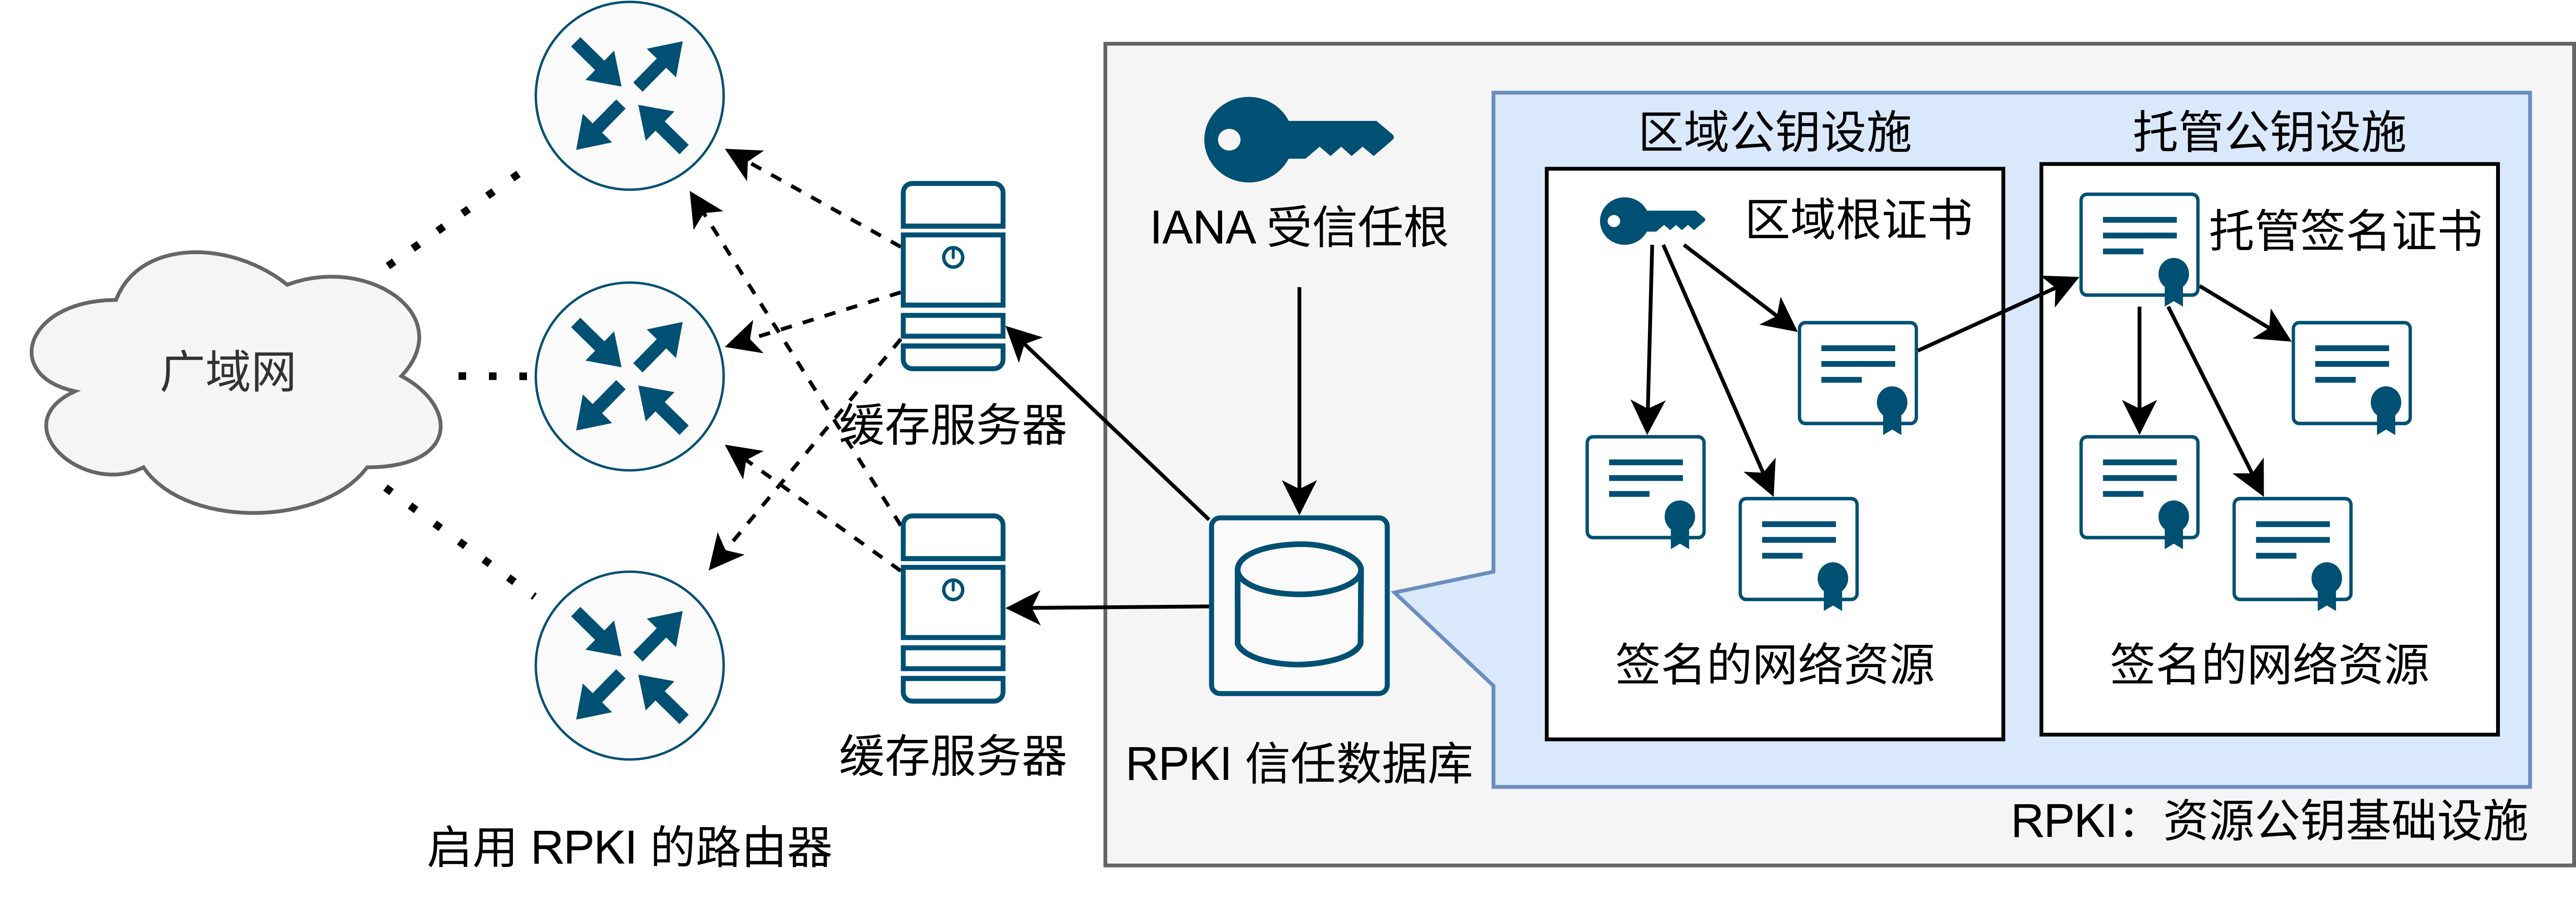
\includegraphics[width=0.9\linewidth]{chapter/c1_images/c1_rpki.png}
    \caption{RPKI 原理}
    \label{c1_rpki}
\end{figure}

然而它在 2013 年被提出至今,并未能有效避免广域网络中的路由异常,尤其是具有恶意目的的蓄意攻击;恰恰相反,无条件的信任机制反而引起了更多基于 PKI 机制的攻击。造成如此结果的原因主要有以下几点:

\begin{enumerate}
    \item 采用有限。RPKI是一个自愿的系统而不是一个强制性标准,并不是所有的互联网服务提供商(ISP)或自治系统(AS)都愿意在自己的网络中应用这一标准\citing{cooper2013risk}。这意味着仍有许多网络和设备没有使用 RPKI 来验证路由信息,这可能使它们容易受到BGP劫持。
    \item 复杂性。RPKI依靠使用数字证书和公钥基础设施(PKI)来验证路由信息。这引入了许多额外的流程,并且需要对 PKI 系统等安全设施进行适当的配置和维护\citing{cooper2013risk},否则会导致安全漏洞的产生。
    \item 人为错误。RPKI的信任模式决定了一些涉及密钥的操作必须人类完成,例如配置和维护 PKI 系统、配置路由验证策略等。\citing{cooper2013risk} 人为错误或失误可能导致系统出现错误,促使路由异常的产生。
    \item 恶意攻击。RPKI并非万无一失,可能会受到旨在绕过或破坏验证过程的恶意攻击。例如,攻击者可以通过入侵网络基础设施来获得有效的数字证书,并利用它来宣告非法的路由,或者对RPKI基础设施发起拒绝服务(DoS)攻击,以破坏验证过程\citing{wahlisch2015ripki}。
\end{enumerate}

因而,许多机构转而研究使用各类模型\citing{biersack2012visual} \citing{sermpezis2018artemis}对全球路由表进行建模,从而对路由异常进行早期预警和可视化分析。

\subsection{基于特征度量的路由异常检测方法}

% 0.8-1 页,包含优点缺点
% 缺陷:专家规则,单一或少量已知特征,很多时候基于已有数据和固定的建模方式。

一段时间内,基于统计特征的 BGP 异常检测被运用在多个运营商上,并取得了显著的成果\citing{al2016bgp}。它们主要分为两种类型:一类是通过时间序列特征寻找路由更新在时间上的关联性\citing{al2015detecting};另一类是从结构化的信息入手,从路径信息中提取包含异常的要素。 

一种朴素的异常检测思路是从类似决策树的 IF-ELSE 逻辑出发\citing{li2005internet},从路由的各项属性中发现异常路由发生时的统计量的变化,例如路由数量,更新数量,撤回数量等,这种方法在几场大型劫持事件中取得了较好的效果。 % li2005internet

根据同样的思路,一项研究通过特征工程的方式从 55 种 BGP 特征中提取出 9 种用于识别路由异常的关键特征\citing{hammood2021using},并指出它们相比其它特征而言在一些事件上更具代表性。 % hammood2021using

从时间序列数据入手是一种普遍的从时间特征出发的思路。例如从 BGP 条目更新的时间序列数据出发,使用自相似性\citing{prakash2009bgp}、指数和对数正态分布等统计学方法\citing{de2011anomaly}寻找重复出现的模式,这对于在时间上较为明显的路由异常而言是合适的思路。  % prakash2009bgp

而从结构化的特点入手则是另一种进行异常检测的方式。一种研究方法建立在路由目的地的所属地理信息上\citing{theodoridis2013novel},认为 AS Path 中出现的自治系统地区属性的频率和偏移与 BGP 可能的劫持相关联。 % theodoridis2013novel

而 AS Path 的高阶表示也能够反映出一定的异常特征。一项研究表明,通过发现监督学习中高阶路径的模式,能够对 BGP 事件进行有效的分类\citing{ganiz2006detection}。 % ganiz2006detection

以上方法大多声称自己具有较高的准确度,并已经在一些历史上存在精确记录的路由异常事件的数据集上得到了验证,然而,它们的缺点也比较显著:受限于现有的 BGP 异常历史数据、单一或少量已知特征和固定的拓扑模式,在面对更加复杂的网络环境时性能衰减非常显著。

\subsection{基于时序机器学习的路由异常检测方法}

% 0.8-1 页,包含优点缺点
% 缺陷:基于时间序列,不包含拓扑信息,存在误判可能,很多时候的路由劫持并不基于时间上的数量或单一指标特征。

由于传统基于特征度量的模型无法实现更新,为了能够在未知数据上获得更好的异常检测效果,一些以机器学习为基础的方法被提出。\citing{al2016bgp}它们主要从数据的时间序列特性上入手,通过相关统计量寻找潜在的异常时间点,其中长短期记忆单元(LSTM)与小波变换(Wavelet Transform)\citing{edwards2019border}是一类较为常见的方式。

利用 LSTM 神经网络对时间序列数据的敏感性,广域网路由表的更新能够被视为一个多维的流量时间序列\citing{cheng2016ms},并在时间的滑动窗口中从历史特征里学习潜在的模式\citing{al2012machine},在设置适当的时间尺度的情况下能够对路由异常做出精准的判断。  % cheng2016ms

小波分析在面对具有尺度缩放特点的时序数据上具有优势,因而通过 BGP 更新消息的时间方向自相似性能够借助小波变换对网络中的异常进行识别\citing{mai2008detecting},并通过聚类的方法缩小异常发生的范围。 % mai2008detecting

通过机器学习的时间序列方法构建的异常检测模型主要是将路由更新数据作为多维度的时序变量进行处理,因而在针对大规模路由异常数据上拥有较高的准确度。\citing{sriram2009comparative} \citing{theodoridis2013novel} 然而,这些方法同样存在特征不足的弊端,它们在将原始数据集转换为时间序列的同时,意味着丢弃了网络数据中的拓扑信息,此外,很多情况下,路由劫持并不一定影响全部的网络,事实上,大规模的路由异常往往是罕见的,利用基于时间上的数量或单一指标特征进行异常检测并不可靠。

\subsection{基于图网络的路由异常检测方法}

% 0.5 页,包含优点缺点
% 缺陷:本质上还是时间序列数据的特征变化,或没有考虑到路由算法本身基于路径的特点(BGP 的其它特征,例如 community)。

近年来,有研究开始尝试通过基于图的方式解决广域网的路由异常检测问题\citing{al2016bgp},将网络路由信息带入图的范畴。其中一种方式是利用相似度和相关性特点,将路由更新的相关指标间的依赖关系使用图网络来表示,此类做法事实上仍然基于时间序列数据特性的做法,存在与上述基于时序数据的模型一致的问题\citing{hoarau2022bgnn}; 另一种方式是使用在图上具有拓扑学习能力的 GNN 来解决异常检测问题,已有研究对此思路做出调研\citing{peng2022multi},实验证明使用基于图网络的机器学习方法来解决此类问题是具有研究前景的。% hoarau2022bgnn

将路由模型视作图网络是一种合乎逻辑的方式:广域网络的拓扑自身即是一类图网络\citing{sanchez2019comparing}。然而,模型没有考虑到基于路径本身的非拓扑属性(BGP 的其它特征,例如路由的社区属性),是当前使用图网络算法解决路由异常问题的一个常见的问题,同时由于路由数据的复杂性,仅采用传统的图神经网络的方式难以处理稠密且庞大的互联网路由数据。

\section{主要研究内容}

% 0.8x3 页
\subsection{基于海量路由数据的图网络数据生成算法}

路由数据集中包含有关自治系统路径的信息,这些基于拓扑的信息能够在图的角度准确描述路由的传播特性,在异常检测中利用这些信息能够摆脱将广域网的路由更新看作时间序列数据的思路,从而提升模型的性能。对于结构化有序数列的数据集合而言,常用的方法是将其转换为图网络,并使用基于图的算法来获得对应节点的表征,进而进行异常检测。

在使用一种类型的数据集时,应当首先考虑数据适用于哪些基本算法结构。把当前广泛使用的路由数据集应用到基于图网络的表征学习架构上时,将会面临两类影响图网络模型性能的问题。其一,由于这些数据集寻求对图网络尽可能的全面覆盖,单一的数据集并非由单一来源提供,因而数据集中存在冗余的路由,临接矩阵过于稠密,这些冗余路由可能形成大量重复链路,进而干扰图网络算法的权重,或是增加图网络计算的复杂度,影响检测效果。其二,由于数据集最终是由自治系统通过路由反馈协议提交的,广域网路由数据集本身可能存在大量能够被图网络算法视为噪声的连边,例如对等路由和无效路由,这些噪声能够很容易地影响图中节点的指标,例如中心度、临接节点等,可能导致图模型失效。

为解决上述问题所提出的挑战,本文提出了一种通过网络路由数据生成符合一定结构特征的图网络的算法。该算法首先从广域网的架构层面出发,分析了可能干扰数据集的路由的特点,针对图网络中存在的噪声,引入了对等路由的的概念,并通过实验证实了广域网络路由在图的角度是可以分解并分离一部分噪声的。通过上述方法,能够从未经处理的广域网数据集中提取出更适合图网络算法、保留原数据集大部分拓扑信息的图网络数据。最后,作为与之对比的模型,还研究了一种利用节点相似度重新生成相似度网络,并由此构造稀疏网络的方法。

\subsection{基于属性信息聚合的广域网络路由异常检测研究}

传统的基于图卷积网络的模型通过多个卷积层聚合图网络节点的各阶邻居信息,从而得到各个卷积层的嵌入输出,而广域网络中自治系统之间存在由路由路径维持的关联性。因此,在考虑基于广域网络路由的数据集时,使用基于邻居特征的模型是一种值得思考的解决方法。

图卷积涉及到对邻接矩阵的多次乘积变换,这对于数据量较大的场景而言具有挑战性。事实上,由于广域网络的图数据过于庞大,已使得使用传统图卷积网络的方法不可用。此类问题通常要求对图网络进行采样,聚合节点及其邻居包含的信息,从而降低需要处理的矩阵维度,达到降低运算量的目的。在广域网络路由的数据集上,如何正确的对采样和聚合过程进行建模,以达到良好的预测效果,是研究面临的一个挑战。

本文对于上述问题提出了一种解决思路,基于 GraphSAGE 模型上实现了一种基于路径的采样聚合方法。具体来说,首先本文引入了 GraphSAGE 的基本框架,以便模型能够在海量路由的数据集上得以学习和更新,随后,本文分析了 GraphSAGE 常用的聚合方式和损失函数,从而提出了一种从路径特征中选择权重的策略,它能够利用数据集中的路径方向的特点对邻居信息进行聚合,从而更加适用于广域网络路由的数据集。

\subsection{基于随机游走特征嵌入的广域网络路由异常检测研究}

一般而言,图网络算法会首先进行数据的构图,然后在图网络上进行进一步的学习任务。然而,根据广域网络的选路规则,自治系统相互发送的路由应当是当前观测角度下的最优路径,即最短自治系统路径,这意味着网络路由数据集与一般的图网络数据集相比,还在路径方面存在一些特征,构图操作能够提取路径上的拓扑关系,但在此同时也会丢弃路径集合本身所携带的一些与数据集中路径的分布状况有关的信息。如何将这部分信息在构图前利用到后续任务中,或是直接绕过构图步骤进行建模,是一个值得关注的问题。

基于随机游走的嵌入算法即是一种与之有关的模型,这类算法的嵌入模块接受一组采样路径,采样方法遵循一定的随机规则,其中的代表包括 node2vec 和 path2vec,而后者恰好是一种对最短路径进行表征的方法。在将路由数据集应用于这类模型之前,还需要解决两个问题,其一是如何保证输入到嵌入模型中的采样路径的分布状况与特定的随机游走方式相同,其二是如何将网络路由数据集中其它与拓扑无关的属性利用在后续的异常检测上。

针对以上问题,本文提出了一种新颖的随机路径采样模型。具体而言,首先通过基于路径的数学分析,提出了两个重要的前提假设,确保通过随机采样路径能够准确学习到网络的拓扑特征,并通过实际数据和分析验证了其合理性,随后,本文引入了随机游走中心度的度量方式,并将其运用在了随机路径的采样上,这种采样方式能够根据路由选择规则采样,进而平整化输入数据的分布状况。最后,通过上述方式构建了一套完整的异常检测模型。

\section{论文的结构安排}

本论文主要由以下几个部分组成:

\textbf{第一章} 是本文的绪论。本章节首先结合当前工程上的需求,介绍了本论文的研究背景,并从理论和实际出发介绍了本论文的研究意义;随后,系统性地介绍了与本论文研究内容相关的、国内外的研究现状和工作进展,并对其给出了概括性的总结;最后,该章节简单介绍了论文的四个大方向上的研究内容和总体结构。

\textbf{第二章} 介绍相关概念,该章节首先简述了广域网络的架构及路由异常涉及到的相关概念,随后针对本论文中涉及到的几种基础图网络异常检测方法进行概述,最后对后续章节将涉及到的中心度,尤其是随机游走介数中心度进行了介绍。

\textbf{第三章} 是本论文的第一个研究内容,基于海量路由数据的图网络数据生成算法。该章节首先简述了当前网络路由数据集的现状和不足之处,随后从数据自身结构角度进行了分析,提出了一种降低冗余和无关路由的图网络生成算法,最后对由算法获得的数据集的参数进行了对比实验分析和可视化。

\textbf{第四章} 是本论文的第二个研究内容,基于属性信息聚合的广域网络路由异常检测研究。该章节首先介绍了经典图卷积网络存在的计算复杂度问题,然后对 GraphSAGE 进行了介绍和分析,进而提出新的基于路径的采样和聚合方法,并在此基础上进行了对比和消融实验。

\textbf{第五章} 是本论文的第三个研究内容,基于随机游走特征嵌入的广域网络路由异常检测研究。首先对采用的基本模型和特征度量方法进行了介绍,随后对问题进行了分析和转化,然后详细介绍了模型的基本架构,最后,在多个数据集上进行了实验和分析,并针对单个样本进行了案例分析。

\textbf{第六章} 对全文的研究工作进行了总结,并对未来的研究方向和技术发展进行了展望。

% 0.5-1 页



\chapter{相关概念}

% 7-9 页


\section{广域互联网络的路由架构}

\subsection{广域网络的结构组成}

广域网是横跨国家、地区的、相互连接的全球性网络系统,如此庞大的体系决定了它必定将使用分布式的方式组成和管理,参加广域网络的组成部分依照一定的规则交换确认彼此的身份,并同时交换路由信息\citing{douzet2020measuring}。

\subsubsection{基本组成与管理方式}

互联网的基本组成单元是其中的成员网络,它们是能够被是作为一个行政实体的,一组或一个处于相同或类似策略管理下的路由器和终端设备,被称为自治系统(AS)。自治系统内部通过内部网关协定(IGP)交换系统内部的路由条目,而数以万计的自治系统相互独立建立自己的连接,并通过外部网关协定(EGP)在广域网层面交换彼此整个系统的路由项目,其中边界网关协定(BGP)是广域网络中唯一公认的外部网关协定\citing{rekhter2006border},因此后续的路由异常问题分析均以 BGP 协议为基础进行。

与通过 IP 地址确定设备的网络地址类似,BGP 协定使用一种称为自治系统编号的唯一标示符来确定一个自治系统的身份,它的范围是4个字节(0-4294967295)\citing{rekhter2006border}。在互联网中,互联网号码分配局(IANA)负责管理这些号码及所属于这些自治系统的 IP 地址的的分配,它通过一种层次结构将这些资源分配给五个区域互联网注册局(RIR),而这些注册局则通过本地互联网注册局(LIR)向下分配获取的资源和网络号码\citing{angieri2019distributed}。

\subsubsection{商业网络的层次结构}

在互联网中,路由信息的传递并不一定是无方向的。在实际的互联网络中,大部分具有较多直接连接或具有更优质线路的网络是商业公司,它们将向具有更低连接性的网络及其客户网络提供付费的连接服务,这直接体现在了路由信息的传递上,在与网络路由相关的研究中,这类单向的信息传递通常被称为非对等互联(Transit)\citing{gregori2011bgp}。

由于上述原因,互联网的路由结构从最初设计的完全分布式逐渐地转变为了具有了一定层次和中心性的结构\citing{vanbever2009hierarchical}:一些网络能够经由更少的自治系统,从而抵达互联网的每一个角落,它们被认为具有更高的中心度。

因而,有研究提出了“客户锥形”的概念\citing{luckie2013relationships}:一个自治系统的客户锥形是它自身和在广域网中能够观察到的通过非对等互联路由可以到达的所有AS,即它和它的任意阶客户。

% 来个公式

对于一个自治系统而言,位于它的客户锥形中的自治系统的路由一般会直接或间接地经由它,因而这项指标展示了它对网络资源的控制能力\citing{luckie2013relationships},即能够影响到网络中的哪些部分的路由。在一些研究中,它的大小常常被用作一种衡量标准,用于度量自治系统的相对规模\citing{doverspike2010structural}。

与此同时,一些网络常常还会与其它网络建立互利且双向的路由交换,相互直接交换各自的路由信息,通常任何一方都不向对方支付费用,这种关系被称为对等互联(Peering),通常这类对等路由不会继续发送给对等方以外的自治系统。\citing{vanbever2009hierarchical} \citing{luckie2013relationships} 在一些被称作互联网交换点的设施内,会有大量 AS 形成近似于全连接(Full Mesh)的对等互联关系,据调查显示,对等互联大大降低了流量结算成本,并降低了互联网日益提升的中心度\citing{luckie2013relationships}。

\begin{figure}[h]
    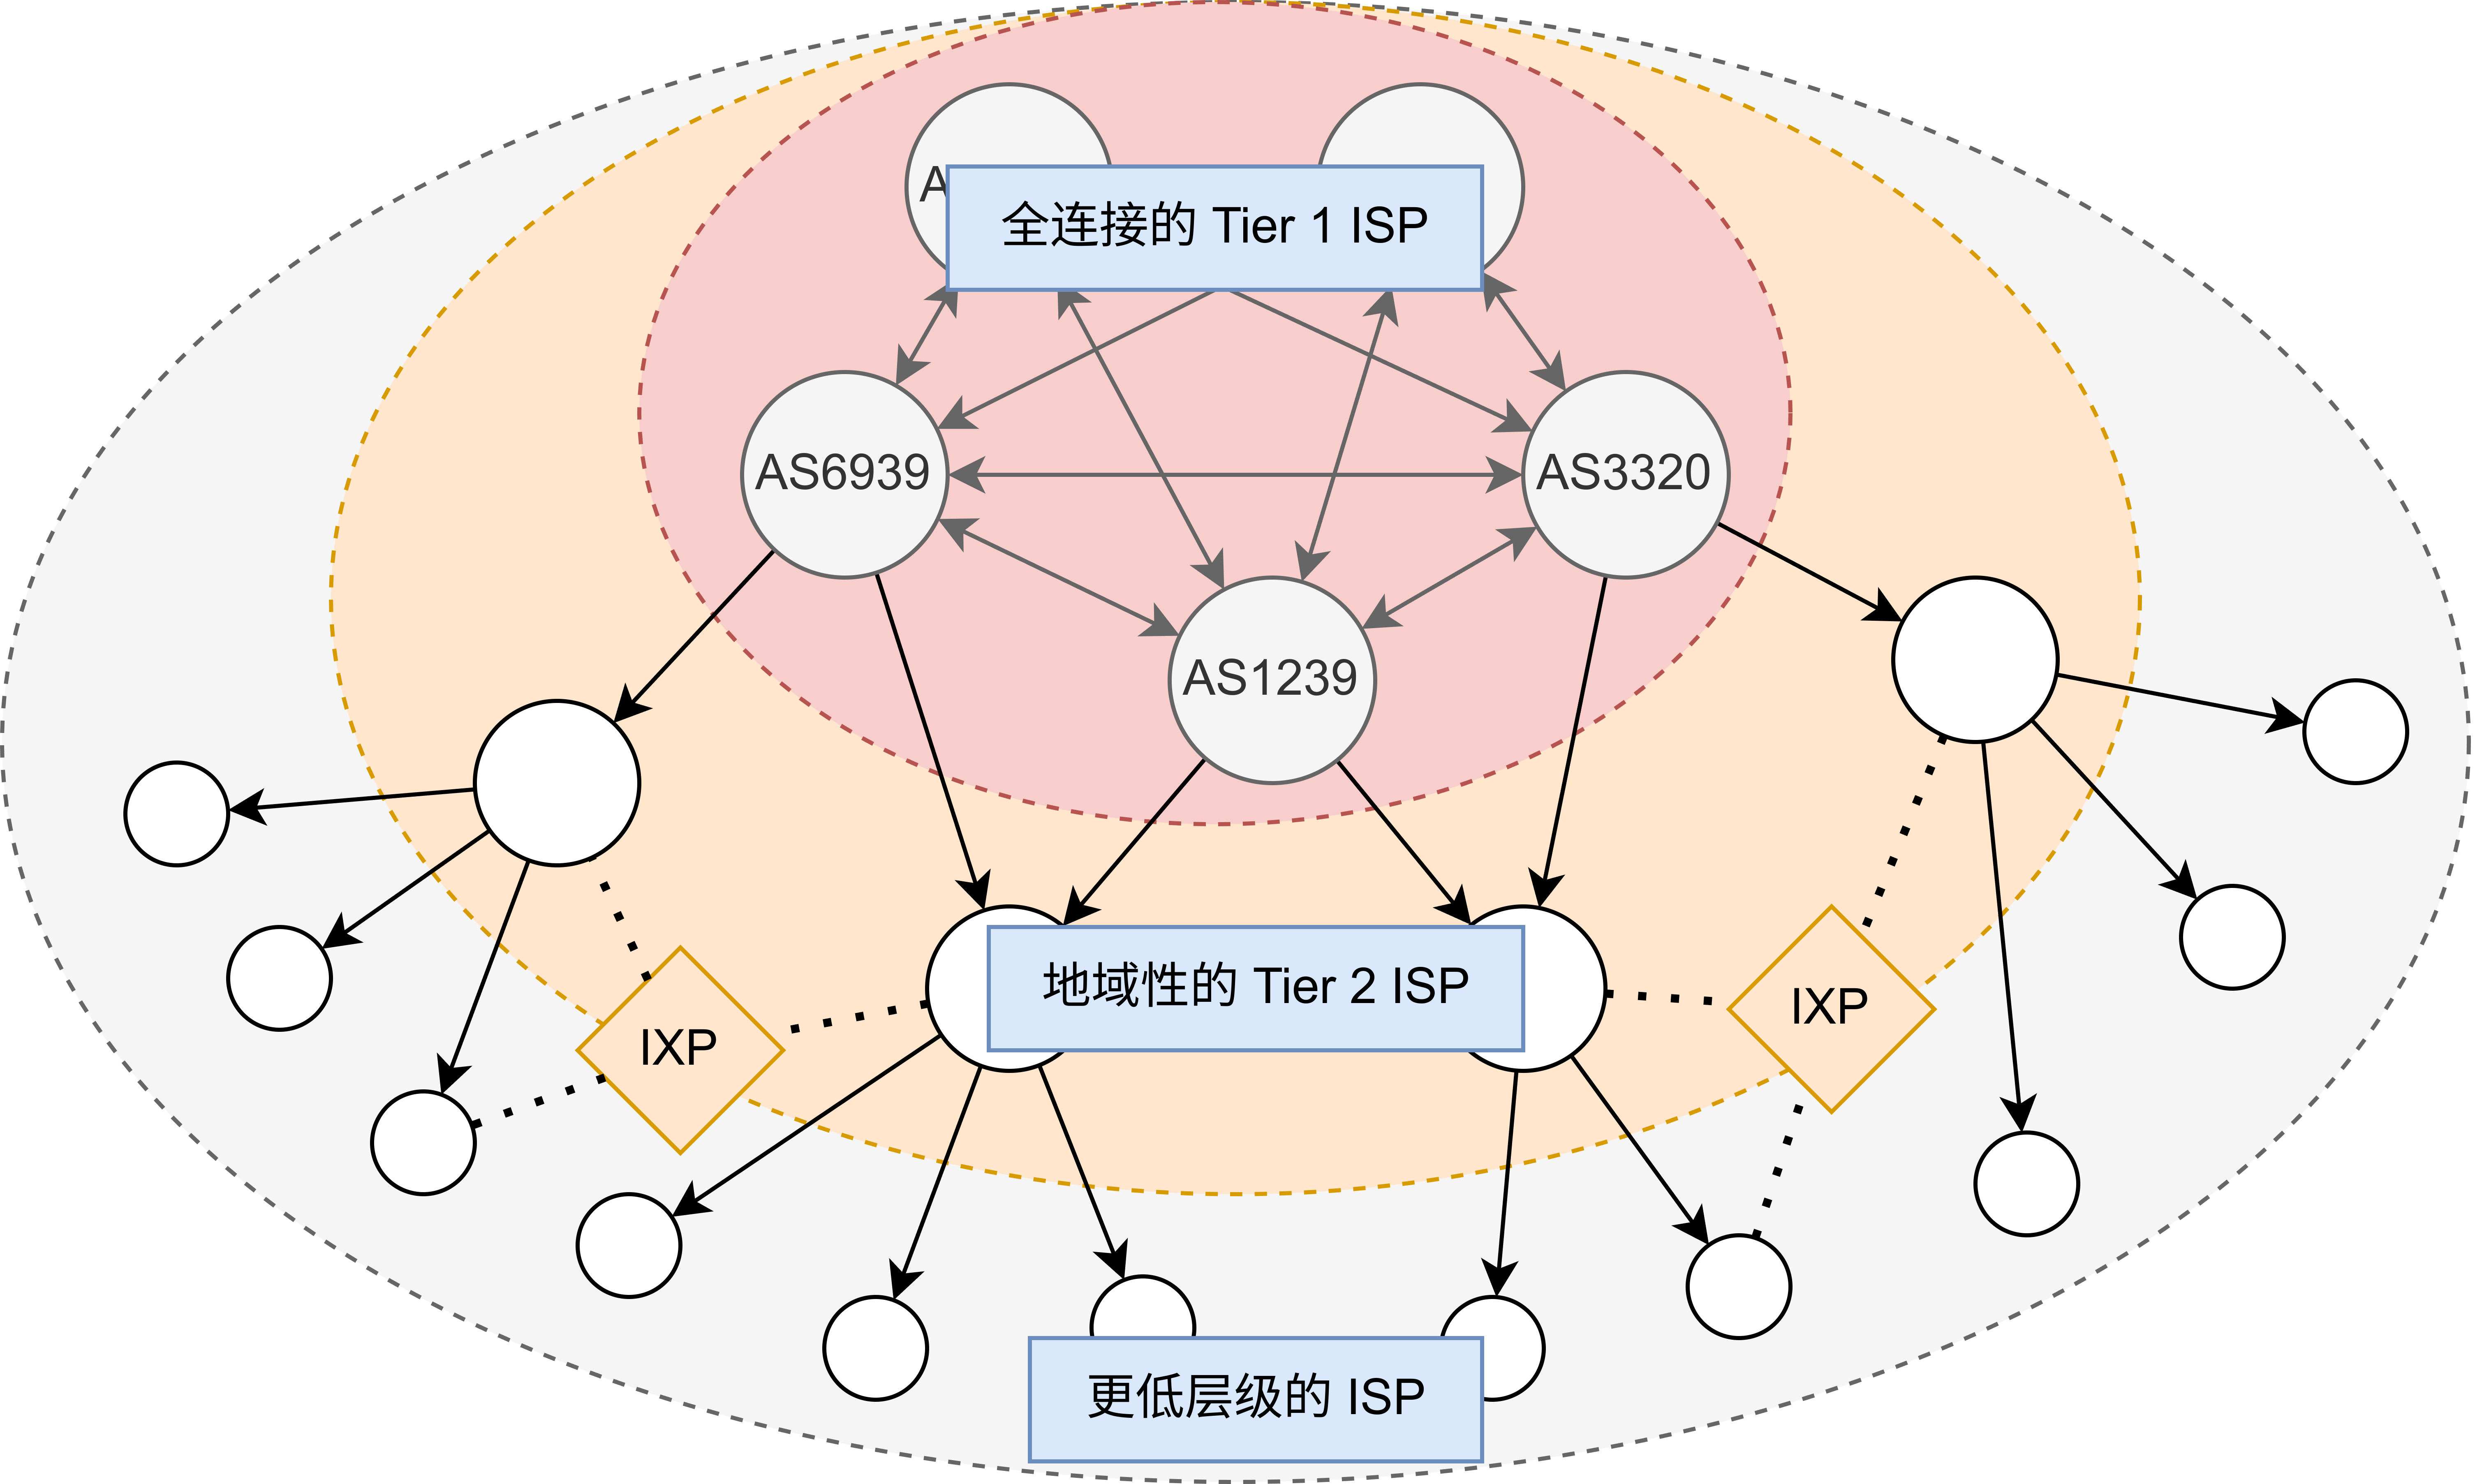
\includegraphics[width=0.7\linewidth]{chapter/c2_images/c2_wan-asn-structure.png}
    \caption{广域网络的层次结构}
    \label{c2_wan-asn-structure}
\end{figure}

图 \ref{c2_wan-asn-structure} 更加直观地展示了互联网中存在的三级层次结构\citing{doverspike2010structural}:彼此相互全连接(Full-Mesh)提供非对等互联路由(事实上即是全部网络路由)的I类自治系统(Tier 1);直接由I类自治系统提供非对等互联路由的II类自治系统(Tier 2);间接通过上级自治系统访问全部网络的III类自治系统(Tier 3);这些自治系统还直接或通过互联网交换点间接进行对等路由的交换。

\subsubsection{分布式网络的对等结构}

在互联网之外,还存在一些社区维护的实验性分布式网络\citing{mirz2018distributed},它们的大部分网络通常是双向提供非对等互联服务的,即在对等互联会话中交换全部已知路由,因此在结构上具有截然不同的特点,例如由于不存在商业关系,整体上具有更少的中心度、成员自治系统的组织一般不具有层次性。

中国教育和科研计算机网(China Education and Research Network,简称 CERNET)\citing{li2011china}是我国教育部、赛尔网络与众多国内高校合办的实验性网络。虽然 CERNET 本身是互联网的参与方,但它的成员单位大多拥有自己的自治系统号码,并相互通过 BGP 协议交换自身的路由,因而在内部能够被视作为一个分布式广域网络。

DN42(Decentralized Network 42)\citing{dn42us}是一个由社区发起的的去中心化网络。 与一般的网络不同的是,DN42 拥有着与其他网络相独立的地址空间、自治系统编号规则和域名系统,因此其架构完全独立于互联网,并且其参与方通常使用重叠网络(Overlay Network)技术,通过底层网络建立网络隧道与其它自治系统相互连接,而非借助光纤或网线的方式通过物理介质连接,这样的组网方式降低了网络的申请门槛,因而在尺度上具有一定的规模,适合用作网络相关研究。

\subsection{广域网络中的路由协议原理}

由于 BGP 协议在自治系统间的广泛性和通用性,广域网络中的路由在通常情况下指使用 BGP 协议在广域网中交换的路由,它与内部路由协议不同,不使用常见的最短路算法,而是让每一个自治系统保留一份当前视角的全球路由表,并直接根据路由表中的属性选择路由\citing{rekhter2006border}。以下将介绍它的基本原理。

\subsubsection{路由信息交换}

由于广域网的分布式和开放性,使得它的路由不存在用于统一调度和管理的中心机构,这使得它具有强大的纠错能力。即使自治系统之间没有直接连接,或是直接连接因故断开,边界路由协定会帮助路由器寻找替代路径,虽然可能在传输延迟、带宽等受到限制,但是仍然能够正常通信\citing{verma2018analysis}。总的来说,互联网的分布式系统理论上是具有良好的鲁棒性的。

自治域内通过内部路由协定交换的域内路由通常不会传播到自治域外,并且具有更少的层次结构,而由于处于统一管理之下,网络拓扑结构上的变化是可预测的,因而此类路由一般不会出现异常。而每个自治域之间的路由则由自治域间的链路状况、主机状况,甚至是政府的监管审查、贸易壁垒等非技术因素而决定,所有自治域共同组成分布式系统,互联网这一整体将随着各节点的情况改变而不断改变自身的拓扑结构,位于自治域之间的、通过边界路由协定交换的域间路由也将随之变化\citing{al2016bgp}。因为其路由条目属性过多、路由选择策略较为复杂,常常因为外界因素出现异常状况。

\subsubsection{路由选择算法}

与统一管理的内部路由协议不同,为了保证路由系统的所有参与者都能够自行决定最优路径,BGP 协议要求路由条目中的属性信息尽可能地能携带自定义的字段,并被任意途径的自治系统说采用。

% 总的来说,它包含四种类型的属性信息:

% \begin{enumerate}
%     \item 众所周知的强制属性:所有自治系统的路由器都能识别并处理,并且字段必须被包括在传递的每一条路由信息中。
%     \item 众所周知的可选属性:所有自治系统的路由器都能识别并处理,字段能够可选地被包括在传递的路由信息中。
%     \item 可选的传递性信息:能够被一些自治系统的路由器识别并处理,即使不能识别,也需要被包括在进一步转递出去的路由信息中。
%     \item 可选的非传递性信息:能够被一些自治系统的路由器识别并处理,它们能够被忽略掉,不被包括在进一步转递出去的路由信息中。
% \end{enumerate}

以下是协议中最常见的两种属性信息,它们将在后续章节的研究中使用:

\begin{enumerate}
    \item 自治系统路径(AS Path)\citing{rekhter2006border}是一种强制编码在路由条目中的信息,它表达了路由在自治系统层面的传递信息,可以被理解为一条由节点 ID(自治系统编号)组成的有向路径。每个自治系统在将路由信息转递前,都会在此路径的首部添加自己的AS号码,以防止路由循环。
    \item 社区(Community)\citing{donnet2008bgp}是一类可选的信息,它能够理解为这条路径所关联的标签,这类标签信息既可以是私有的(只在某些自治系统有效)也可以是共有的(一些预定义的属性会在所有自治系统生效),路由消息在传递的时候,自治系统的路由器能够根据规则去添加、删除和改写这些标签。
\end{enumerate}

与内部网关协定中复杂的权重不同,由于自治系统之间难以统一协调,加之过于巨大的网络拓扑使得精确的路径寻找较为困难,一般情形而言,广域网的 BGP 协议寻路使用最短自治系统路径,同时使用社区属性对一些需要特殊优先级的路由进行调整。

自治系统路径能够反映出路由中的拓扑信息,而社区属性是对整个路径的标签信息,通过这两个信息能够构建出一个有向带权重的图。由于其它信息在不同自治系统下具有不同的数值定义,因而无法仅通过数据集确定意义,故无参考价值,本文不再介绍。



\section{广域网络路由异常}

\subsection{路由协议的固有缺陷}

广域网络的路由事实上是非常脆弱而易受攻击的。实际上,BGP 最初被提出以来,没有任何被协议所直接包括的安全机制\citing{mitseva2018state},路由的稳定可靠完全是基于网络运营商之间的信任和恰当的设置,也即假定系统永远不会出现随机故障或安全问题,路由器之间不会发送错误的数据。这引入了一个明显的漏洞:如果路由协议的其中某个参与方出于恶意,试图通过BGP协议影响其它自治系统乃至全球的路由表,其它的自治系统没有任何通用的手段来阻止它的发生。

在 1998 年,RFC2385 对 BGP 引入了密码保护机制\citing{heffernan1998protection},解决了通过二层链路劫持 BGP 会话的可能性,但它使用易受攻击的 MD5 加密,至今尚未更改。1999 年,RFC2439 对 BGP 引入了路由震荡抑制(Route Damping)\citing{villamizar1998bgp}机制,缓解了 BGP 的路由震荡问题。然而,在标准提出的几十年来,广域网络上的路由异常问题从来没有得到根除,究其原因有二:

其中一个原因是针对底层协议和标准的修改难以被普遍采纳。一项报告指出,互联网运营商的核心设备的更新周期长达 10-15 年,并拥有相当大的方差\citing{mahimkar2010detecting},这意味着在新的标准提出后,大部分设备都很难短时间内进行引入\citing{mitseva2018state},或是为了与其它互连的运营商兼容的原因关闭这些增强安全性的功能。

另一个重要原因是,这些手段事实上并未解决来自恶意的路由协议参与者和不遵循规范的配置者的安全威胁\citing{sermpezis2018survey}。基于信任的广域网架构仍然坚持默认所有路由参与者不会存在恶意破坏的可能性,这是维持互联网分布式的基础。

因而,由此产生的安全性问题,包括路由异常问题,便从标准性问题转变为了无法避免的问题,它的潜在安全威胁使得对路由系统的安全性的建模研究更具意义。

\subsection{广域网络的潜在安全威胁}

% \subsubsection{路由震荡}

% 路由震荡是指由于物理故障、系统错误、人为因素等原因,所造成的路由表的频繁变化。相互连接的分布式网络会因此不断向相邻自治系统宣告和撤回路由,导致其他节点频繁重新计算路由。这会对整个网络造成严重的算力和链路负担,轻则网络延迟升高、不稳定,重则导致拒绝服务攻击(Denial of Service,DOS),并造成大规模的网络服务瘫痪。

% 这样的问题可以通过修改外部网关协议的行为,来防止系统资源的枯竭,例如在 BGP 协议中启用路由震荡抑制功能,临时关闭反复路由更新的邻接系统的 BGP 会话,或是限制对应协议的更新频率。

% \subsubsection{路由劫持}

路由劫持是广域网中最常见的安全威胁。当一个自治系统因为配置错误或恶意行为的情况下,它会宣告并不应由它宣告的路由条目,如果它的邻接系统没有部署 RPKI 机制或是没有强制启用路由的过滤机制,这些错误的路由条目就会通过 BGP 会话传播到它的邻接系统,并进而被发送至整个广域网内所有可达的边界路由器中,这时候路由劫持事件即被触发,由于 BGP 路由协议的规则影响,目的地涉及到被劫持的 IP 地址块的网络流量有可能会被路由至发起劫持的自治系统\citing{mitseva2018state}。而现代互联网的系统反应时间非常迅速,根据一项调查显示\citing{sermpezis2018survey},被劫持的路由条目能够在 10 秒时间内抵达全球 90\% 以上的互联网系统。

并非所有的 BGP 劫持都能够成功造成安全危害,事实上,对网络的拓扑结构造成更大影响的 BGP 劫持通常能有能力影响更多或具有更大客户锥形的自治系统,这通常有两种方式:

\begin{enumerate}
    \item 发起劫持的自治系统宣告前缀长度更长的路由。网络系统的路由层次性决定了路由器在接收到更准确的IP地址块的路由信息的时候,会直接采用并完全弃用任何路径选择算法。
    \item 提供更为直接的自治系统路径,利用广域网路由选择算法的特点,构造出比正常路由更短的自治系统路径,这将使得路由器认为该路由在逻辑上更优。
\end{enumerate}

% 大型网络或网络群的运营商(其中很多是ISP)会明目张胆地进行这种恶意活动,这似乎令人惊讶。但考虑到据统计,现在全球有超过8万个自治系统,有些自治系统不值得信任也就不足为奇。此外,BGP劫持并不总是那么明显或容易被发现。坏人可能会把他们的活动伪装在其他自治系统的后面,或者宣布一些不可能被注意到的未使用的IP前缀块,以便不被发现。

图 \ref{bgp-hijack} 显示出了一种典型的基于更长前缀的路由劫持,AS3 通过向广域网宣告 1.14.5.0/24 这一更长的路由前缀,劫持了本应属于 AS1 的 1.14.0.0/16 的路由,并将访问 1.14.5.14 IP 的流量引导向攻击者的设备,整个流程中 AS1 及其 AS2 没有执行任何错误操作,同范围的其他 IP 也能通过一种称为流量穿透的方法返回正常目的地,从而实现隐蔽的攻击手段。

一些网络运营商可能因为配置失误,将内部或错误的路由发送至自治系统外,造成BGP劫持,这样的情况常常被称为路由泄露,据调查,此类事件相比于恶性的劫持事故而言往往更加常见\citing{vervier2015mind}。根据一项研究显示,并不是所有的 BGP 劫持事件都能够被注意到并及时采取措施\citing{schlamp2016heap},攻击者可以选择不常使用的地址块,或是未被注册的地址块进行劫持。以上原因都导致了路由异常的检测实质上难以判断是否是恶意攻击行为。

\begin{figure}[h]
    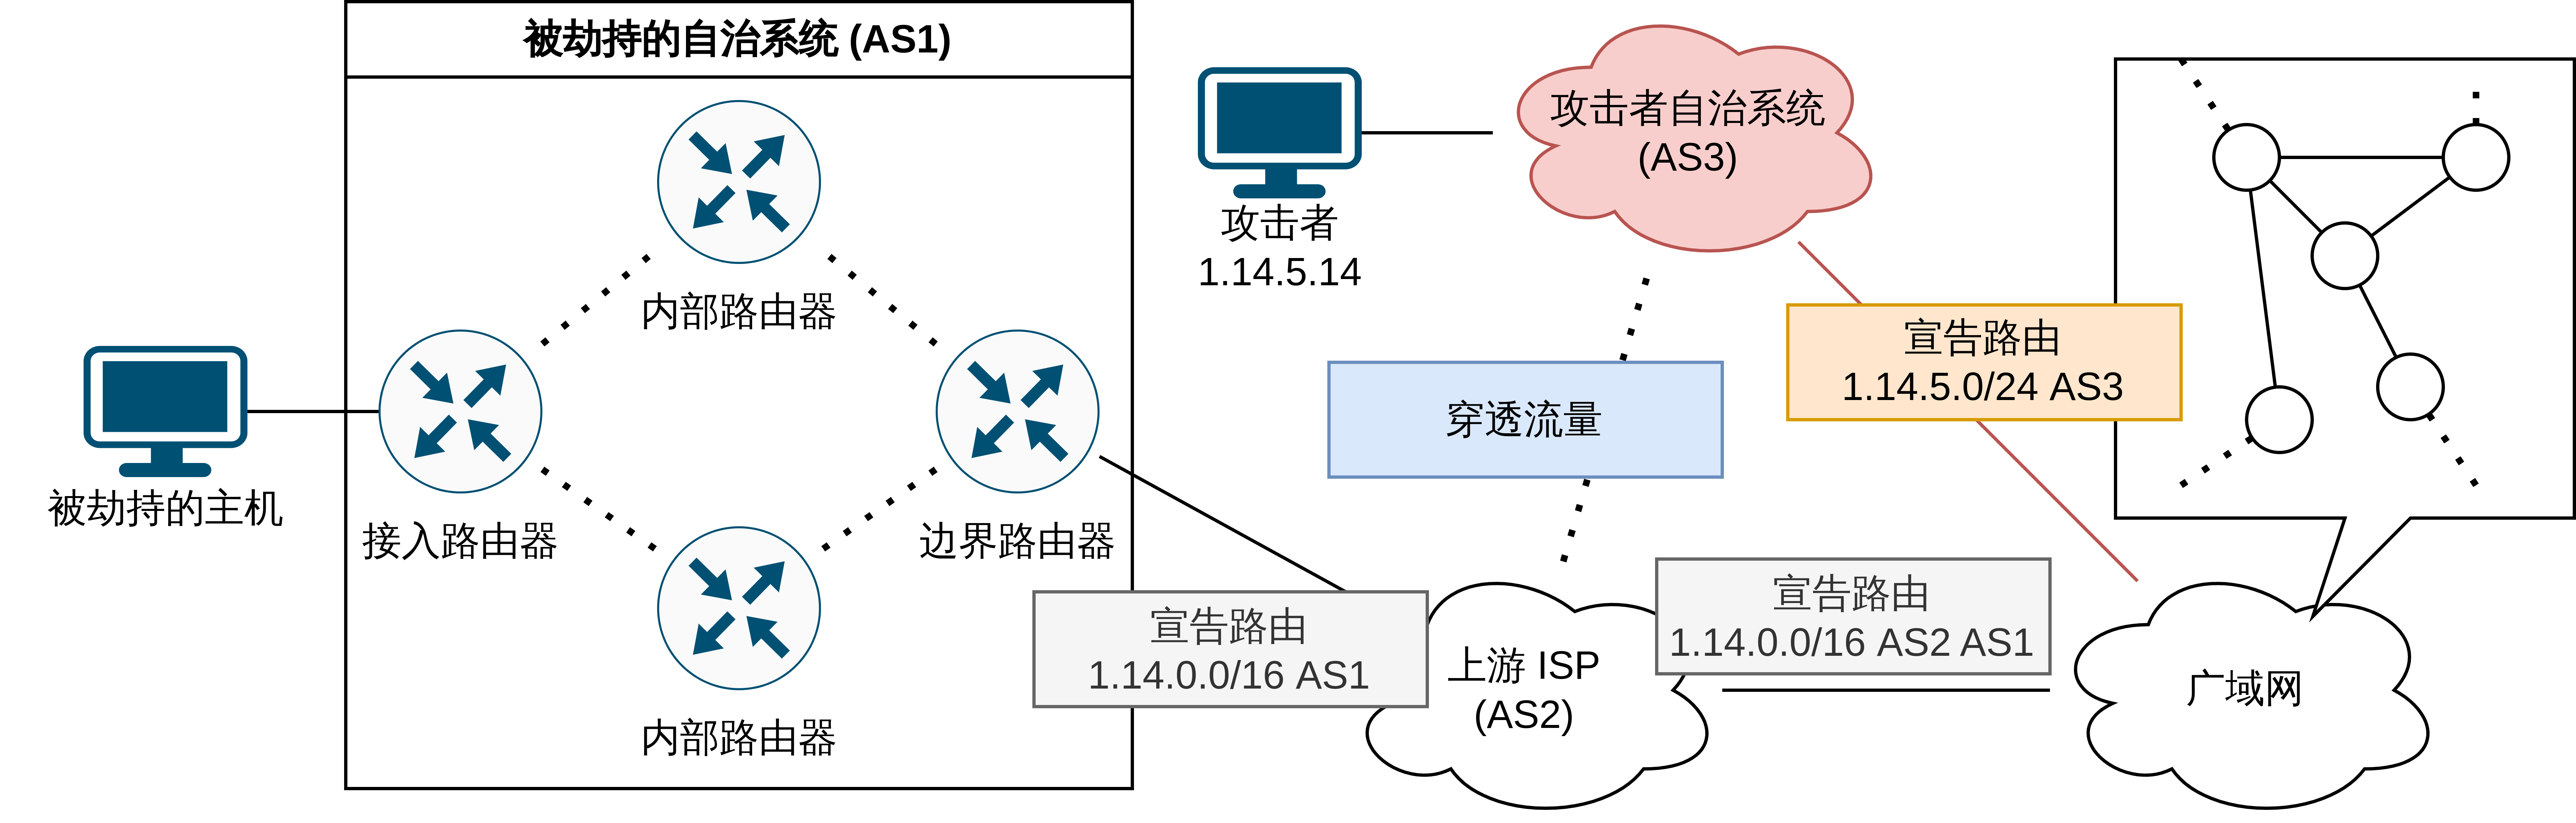
\includegraphics[width=\linewidth]{chapter/c2_images/c2_hijack.png}
    \caption{BGP劫持示意}
    \label{bgp-hijack}
\end{figure}

\subsection{路由异常的定义}

路由异常,被定义为一种表现出异常特征的路由更新条目,它通常携带有异于其它正常路由拓扑的自治系统路径,并有可能在其它属性上呈现出不同的特点\citing{al2016bgp}。它一般包括两类状况,一种是 BGP 劫持,这类事件通常是有害的;而另一类是新路由的增加,由于分布式网络的系统之间常常建立和断开连接,这一类异常状况既可以是突发事件,也可以是可预测的人为因素,它们并不会产生实质性危害。

由于现有数据集中基于图网络的有标记路由异常事实上并不多见,此类问题一般被认为是一种无监督学习问题。

\subsection{问题的图网络表述}

% 使用基于图网络的数学公式描述问题。
下面通过图网络的数学语言描述本研究所定义的广域网络异常检测:

对于一条路由 $R_i$,它包含三种属性,即对应的 IP 前缀 C,AS 路径 P,社区信息 C,即 $R_i = \{ O, P, C \}$,它们共同组成全球路由表 $R_T = \{ R_i \}$。
% 全球路由表 {R_i} , R_i = {O(前缀), P(路径), C(社区)}

前缀 C 是一个标识符;AS 路径 P 可理解为一个不定长的有序列表 $P = \{A_1,A_2..A_N\}$,其中,路由的源自治系统指宣布该路由的自治系统,对应列表中的最后一个元素 $A_N$;社区信息 C 是一个标签集合 $C = \{C_1,C_2...C_N\}$。

% last(P) = origin

定义图生成算法 $f_g$ 为从路由表数据构造图网络数据集的方法,具体来说,$f_g(R_T)=G<V,E>$,其中节点集 V 是路由表 ${R_i}$ 中所有路由路径上的自治系统号码,即 $V = \forall(A_i \in P \in R_i)$,该算法通过 $R_i$ 特征生成一个有向或无向图 $G<V,E>$,它的边集 E 将由算法 $f_g$ 决定。
% 图生成算法 f_g({R_i})=G<V,E> V=all(P)

定义图嵌入算法 $f_e$ 为从图网络数据 $G<V,E>$ 中提取嵌入数据的方法,它对于每一个图元素输出一个 k 维向量嵌入,即 $e = f_e(G<V,E>) = \{ e_i \}$,而图元素可以是图上的所有节点,也可以是边集或是路径集,即 $N = len(V/E/R)$。
% 嵌入算法 e = f_e(G<V,E>)={e_i} N=num(V/E/R)

最后定义异常分数 $f_a$ 是由新的路由和原有的图数据及其嵌入作为输入,输出对更新路由的异常分数以便于最终进行异常检测,即 $f_a(R_n,G<V,E>,e) \in (0,1]$。
% 定义异常分数 f_a(R_n,G<V,E>,e)

广域网络的路由异常检测问题的本质即包含了以下的部分:

\begin{enumerate}
    \item 设计图生成算法 $f_g$,将原网路数据集转换为图数据集。
    \item 设计高效的嵌入算法 $f_e$,将图数据集转换为图元素的嵌入。
    \item 定义异常检测分数 $f_a$,用以检测新的测试样本。
\end{enumerate}


\section{图网络的嵌入算法概述}

由于图网络数据一般具有大量的节点,通常具有较高的维度,因而很难被传统的基于特征的方法处理。而已有的研究证明,节点的低维嵌入在较大规模图网络中,能够作为较好的特征输入,例如节点分类、链路预测和异常检测\citing{cai2018comprehensive}。

图嵌入算法即成为了降低网络维度,并解决该问题的一种方式。图嵌入算法的基本思路是将网络中的节点特征嵌入到维度更低的空间中,并保证在压缩后的向量空间中,相似的节点依然能够更接近,即尽可能保留拓扑的相似度关系。

以下是一些图网络的嵌入算法的概述,它们将在后续研究中被使用到。

\subsection{图的嵌入}

首先介绍图的嵌入的定义。对于一个图而言,它的嵌入是指它的元素的映射。具体而言,对于一个图 $G<V,E>$ 而言,它的节点嵌入是它顶点的映射关系,如公式 \ref{graph_embedding} 所示:
\begin{equation} \label{graph_embedding}
f:v_i\rightarrow y_i \in R^d, \forall i \in [n]
\end{equation}

图的嵌入算法 f 能够保证节点属性在将维度降至 $d(d<<n)$ 的情况下依然能够保留节点之间的相似度关系。同时,也能够通过类似的过程,将图的其它元素(边、路径等)转化为低维向量。

\subsection{GraphSAGE 模型}

GraphSAGE 模型\citing{hamilton2017inductive}是为了解决经典图卷积网络需要大量图数据输入、无法实现归纳学习等特点而提出的特征聚合方法。在介绍 GraphSAGE 模型前先介绍图卷积网络的概念。

\subsubsection{图卷积网络}

图卷积神经网络\citing{kipf2016semi}是一种图嵌入方法,它的主要目标是通过消息传播和更新的方法,使用多个图卷积函数(即多个卷积层),学习一个图卷积函数,用以将自身和邻居的特征聚合,并输出节点的表示。

然而,传统的 GCN 模型在面对大规模数据集上存在诸多问题\citing{gao2018large}。首先,GCN 的嵌入算法涉及到对整个图的特征矩阵进行多层变换,这意味着它自身具有较高的复杂度;其次,训练 GCN 无法实现归纳学习,在每一次模型更新时都需要对整个图进行重新计算。

\subsubsection{基本结构}

而 GraphSAGE 模型是一种利用采样和聚合节点特征,进而实现归纳学习的图网络算法。它的基本思路是利用已有的拓扑信息,对节点的邻居进行采样,并通过聚合函数的方式,将高阶的邻居信息在不同层次上进行聚合,从而得到最终的嵌入,并用于下游任务。

GraphSAGE 通过以下方式进行迭代,从而获得节点的高阶嵌入:
\begin{equation} \label{graphsage_iter_aggr}
h^k_{N(v)} \leftarrow AGGREGATE_k(\{ h_u^{k-1}, \forall u \in N(v)\})
\end{equation}
\begin{equation} \label{graphsage_iter_concat}
    h^k_v \leftarrow \sigma(W^k \cdot CONCAT(h_v^{k-1}, h^k_{N(v)}))
\end{equation}

它首先依照公式\ref{graphsage_iter_aggr}对节点 v 的邻居的 $(k-1)$ 层嵌入进行聚合,然后按照式\ref{graphsage_iter_concat}中的方法与自身 $(k-1)$ 层特征拼接从而得到第 $k$ 层的特征。它在无监督学习下使用针对邻居的对数近似和针对非邻居的负对数近似使得相邻节点尽可能拥有相同的嵌入。

在GraphSAGE模型中,$AGGREGATE$ 即聚合函数\citing{hamilton2017inductive}是最重要的部分,它决定了如何结合采样到的邻居节点的特征。关于聚合函数的选择有两个条件:

\begin{enumerate}
    \item 可导,因为要反向传递来训练目标的聚合函数参数。
    \item 对称,这里的对称指的是对输入不敏感,因为在聚合的时候,图中的节点关系并没有顺序上的特征。
\end{enumerate}

\subsection{随机游走和图嵌入}

\subsubsection{图网络的随机游走算法}

随机游走\citing{pearson1905problem}是一种典型的基于图网络的采样过程,它被定义为一种以特定随机分布在图网络上选取路径的方式。随机游走的输入是一个图 $G<V,E>$,输出一个路径的集合 $\{ P_i|P = Random\_Walk(G) \}$。随机游走的采样规则可由公式\ref{markov_chain}给出,它实质上是一种有限马尔可夫链:
\begin{equation} \label{markov_chain}
p_{t+1}(a) = \sum_{b:(a,b)\in E} \frac{\omega(a,b)}{\Sigma_{a}\omega(a,b)} p_t(b)
\end{equation}

其中,它包含一个用以根据当前信息(图 G 及其节点 V 边 E 的某种度量值及其组合)决定转移概率的 $\omega$ 函数。

\subsubsection{基于 node2vec 的节点表征 和 基于 path2vec 的路径表征}

在通过随机游走获得采样路径后,即可根据这些路径来生成节点的表征。node2vec \citing{grover2016node2vec}即是一种采用此种方法的节点嵌入模型。

在自然语言处理中,基于语句的 Skip-gram 和词袋的 word2vec 模型被用于对句子中的词语进行建模。node2vec 模型则假设图中的节点可以被视作为可用词语的全集,对节点的路径采样能够体现出图的拓扑结构,正如对词语的组织能够体现出语义信息一样。受此启发,将随机采样的路径送入文本挖掘的嵌入模型中能够很好的反映出节点的拓扑特性 \citing{grover2016node2vec}。

path2vec \citing{kutuzov2018learning} 是对 node2vec 模型的拓展,也是 doc2vec 模型在图网络中的对等模型,它拓展了 node2vec 的采样方式,通过预定义的图距离度量方式对节点进行嵌入,进而能够学习到比 node2vec 更加高阶的拓扑结构关系。


\section{图网络的中心度度量}

在图网络中,中心度\citing{rodrigues2019network}是一种很重要的指标,它用以衡量图网络节点在图中以某种度量方式下的重要性或权重。

在图论中,有许多用于衡量图中心度的指标,它们反映了数据集在不同角度上的特征信息。常用的中心度指标有:

\begin{enumerate}
    \item 度中心度(Degree Centrality):一个节点的度中心度是指该节点在网络中所连接的边数或者连接的节点数。该指标通常适用于基于传播效率的场景。
    \item 距离中心度(Closeness Centrality):一个节点的距离中心度是指该节点与其他节点之间的距离之和的倒数。该指标通常适用于基于连接紧密程度的场景。
    \item 介数中心度(Betweenness Centrality):一个节点的介数中心度是指该节点在所有最短路径中出现的频率。该指标通常适用于基于促进整个网络的连接程度的场景。
    \item 特征向量中心度(Eigenvector Centrality):一个节点的特征向量中心度是指该节点与其他节点之间的连接强度的加权和。该指标通常适用于度量节点的相似程度。
\end{enumerate}

通常情况下,在基于路由的互联网络中,介数中心度\citing{liu2013characterizing}更具实际意义,它能够反映对应的网络节点在路由中的控制力和重要性。

\section{本章小结}

本章节主要介绍了本文涉及到的相关技术概念和主要研究内容。在 2.1 节,介绍了广域网络的基本组织结构,是后续章节中涉及拓扑构建的模型的技术基础。本章在 2.2 节引入了路由异常的背景概念和原理,并通过图网络的角度对问题进行了表述。在 2.3 节中,本章还介绍了后续研究将使用到的一些嵌入算法。最后,本章在 2.4 节对图的中心度这一重要度量指标进行了初步介绍,并针对随机游走介数中心度的意义进行了阐述,这项指标在后续章节中被广泛使用。

\chapter{基于海量路由数据的图网络生成算法}

% 8-10 页

% 0.3 页
目前已经有一些网络研究机构和组织提供了自己收集的全球路由表数据集,并且已经在部分路由异常检测的研究中使用。然而这些数据集并不是图网络数据集,存在一些对于图网络而言不易处理的特征,因而大多数研究并非通过图的角度出发,而是简单地将这些数据集理解为路由更新时间序列,从而损失了其中携带的拓扑信息。因此,为了探索在现有路由数据上进行图的构造,进而将路由异常问题转化为完全可由典型图网络模型处理的图数据,本研究结合路由数据的特点,构建了一种图网络数据集生成算法,并通过一些公开可用的网络路由数据集提取出了相应的图网络数据。

\section{研究背景}

% 2 页

\subsection{现有的网络路由数据集}

现有的互联网络路由数据集通常是由中立机构收集和发布的,借助分布式的收集系统和路由反馈会话,此类机构能够从互联网上不同的位置收集全球路由表中的实时 BGP 信息,并将其制作为格式化的数据库进行发布。

由于 BGP 路由条目是以路径的形式呈现,从单个或少数几个自治系统的路由表中获得的路由信息是极为有限的,同时由于最短路径原则在路径上的体现是一类最小/次小生成树结构的叠加,据此构建的图样本将以采样中心呈现类树状结构,不具有普通性,也不是本研究的研究目标。因此,本文只关注以下具有更加广泛的收集覆盖面的数据集。

RIPE RIS 是路由异常分析中一个最常见的路由数据来源,它由若干位于互联网交换中心的远程路由收集器(RRC) 收集和存储来自参与者通过 BGP 提供的路由数据,其中包含了来自数十个国家的上万个自治系统收集的路由信息。一些路由异常预警系统采用了由该项目反馈的实时数据\citing{ripe2021routing}。

RoutesView 项目\citing{denardis2020internet}是另一个类似的大型数据采集工程,它从 1997 年以来不断收集和归档全球互联网路由表的每日快照,并在全球各地与不同规模的网络建立了 BGP 路由收集会话。

几乎所有可用的网络路由数据都使用 MRT 格式\citing{blunk2011multi},它能够完整地记录路由表中的多种路由信息,其中自治系统路径是表现拓扑结构的主要信息,而社区属性则反映了路由的优先级。

\subsection{现有数据集在图网络算法中的不足}

由于现有的数据集大多以 MRT 数据集提供,此类数据集本身是一类随机事件流,不是现成的图数据集,在实际处理上暴露出了传统的路由数据集在面对图网络算法上存在的不足。

其中影响较大的一个因素是重复数据,由于路由收集器的原理是从不同采样点的 BGP 会话中接收全量的路由信息,因此对于每一个网络都存在大量重复且拥有公共边集的自治系统路径,而这些路径的数量并非在不同网络下遵循同一分布,因而影响了图网络模型的性能。\citing{fonseca2019bgp}

同时,数据在图中的分布状况也导致了数据集在图网络中效果不佳。如图 \ref{c3_as-distance} 所示,通过抽取 RIPE RIS 的 200 个节点与其它节点的平均路径长度数据,该图展示了互联网中自治系统间的平均距离及其分布状况,即数据集构建出的图的可能直径,这直观地展现出了数据集中很大一部分网络,事实上由于相距遥远,由一个或几个形成全连接(Full Mesh)或完全图的I类自治系统分隔(图中的红色部分数据)。对于图中平均路径距离的差异可以归结为对等路由的影响,这一点将在后续模型构建中被提及。

\begin{figure}[h]
    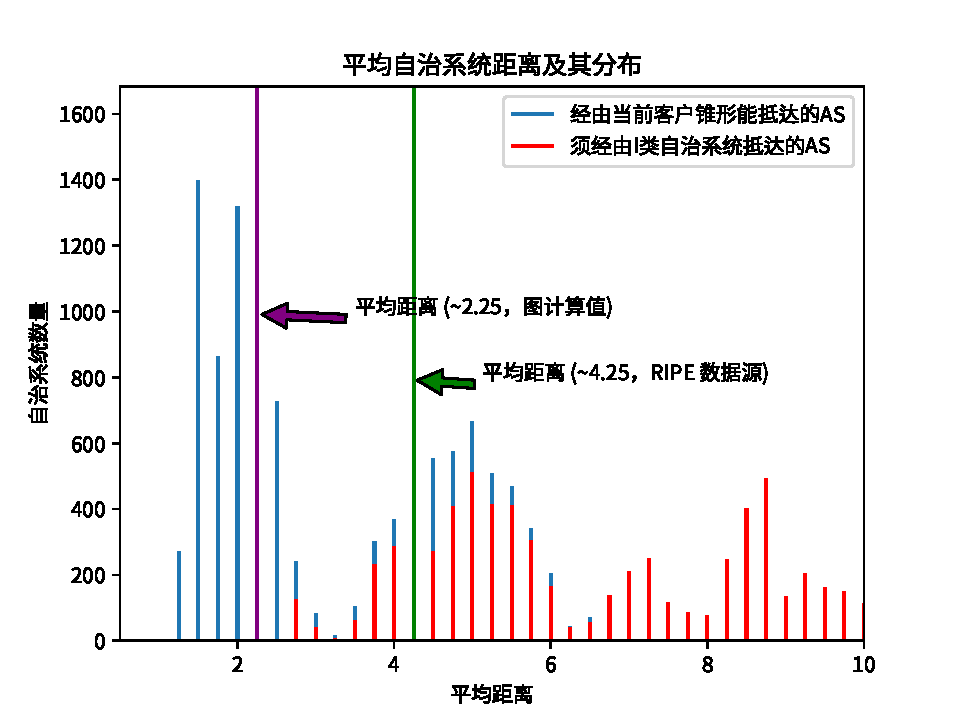
\includegraphics[width=0.85\linewidth]{chapter/c3_images/c3_as-distance.pdf}
    \caption{互联网中自治系统间的平均距离及其分布状况(RIPE RIS 数据集)}
    \label{c3_as-distance}
\end{figure}

图网络所包含的数据量也是一个值得注意的问题,事实上,据2020年一项研究报告称,全球互连网的路由数量已超过 $10^6$ 条,因而由路由数据构造的图大小本身已经超出了一些图网络模型的计算能力,这也是一些研究放弃图网络模型转而使用其它方法的原因。

此外,大部分模型研究的是特定于互联网路由表的异常检测,然而一些社区维护的分布式网络的拓扑结构与此并不相似,这类分布式网络尚未有满足本研究要求的数据集。

因而,从现有路由数据集和分布式网络出发,构建一种图网络数据集的生成算法是很有必要的。

\subsection{研究贡献}

本章从路由协议的角度出发,提出了一种新的路由数据构图方法,能够有效地去除网络中的冗余边和干扰因素,从而降低图的稠密性,使其能够在一些基于嵌入的异常检测模型下获得更好的效果,最后还使用了一些基于图网络的指标和基准算法来评估数据集的有效性,证明了它能够反映出与一般路由数据集相近的特征。

\section{数据获取和图生成模型}

% 3 页

\subsection{数据来源}

先前的章节总结了常见的路由数据集在多样性和尺度上存在不适用于图网络的问题,因此本文将使用来自互联网和 DN42 两种分布式网路的数据。

其中互联网的路由数据来源于 RIPE RIS 的公开数据集\citing{ripe2021routing},它将经过更多的处理步骤以解决数据规模和冗余数据等问题。而 DN42 则是一个去中心化的的实验性社区网络,它的数据集来源于 DN42 全球路由收集器(Global Route Collector)的数据\citing{dn42us}。与 RIPE RIS 相似地,DN42 GRC \citing{dn422022mrt}也提供了 DN42 下几乎全部的路由信息。 

不同的是,由于 DN42 相对于管理规则更为严格的互联网而言具有更加扁平的结构\citing{dn42us},因而具有更强的分布式特点,同时由于其实验性的定位,会更频繁地发生 BGP 路由的异常,甚至能够合规地在一定范围内制造这样的异常以供研究用途,\citing{tsai2022design} 因此本文在互联网之外还使用了这一数据集,在后续的研究中也会借助 DN42 作为一些算法的案例分析。

如表格 \ref{dataset-compare} 所示,本研究采集了相近时间的来自两种网络的数据,并总结了以上两种数据来源的不同之处,可见它们在数据规模、复杂度和结构特点上都有所不同,本研究尝试通过两类截然不同的网络结构的数据集来研究模型在面对不同结构的网络路由上,是否能保持一致的准确度,以便测试模型的泛用性。

\begin{table}
    \caption{两种数据集的参数对比}
    \begin{tabular}{p{0.2\linewidth}p{0.3\linewidth}p{0.3\linewidth}}
        \toprule
                       & \textbf{RIPE RIS}                                & \textbf{DN42 GRC}              \\
        \midrule
        宣告的IP前缀 \newline(IPv4) & $\sim$1,000,000                                  & $\sim$800                      \\
        宣告的IP前缀 \newline(IPv6) & $\sim$170,000                                    & $\sim$700                      \\
        可观测到的自治系统      & $\sim$70,000                                     & $\sim$500                      \\
        更新频率           & 8 小时 (全量),                     \newline5 分钟 (增量) & 10 分钟 (1周内), \newline1 天 (一周外) \\
        网络关系与拓扑        & 对等+非对等                                           & (几乎完全)双向非对等                    \\
        \midrule
        本文使用           & 性能评估                                             & 对照分析                           \\
        \bottomrule
    \end{tabular}
    \label{dataset-compare}
\end{table}

路由收集器提供的数据大多使用 MRT 格式,它能够完整地记录路由表中的多种路由信息,在本章节的研究中,MRT 文件中的路由将在数据的预处理阶段被导出,其中的自治系统路径和社区属性等信息是以图\ref{c3_data-struct}中的形式被保存在层次性的数据结构中,以便于后续将拓扑信息和其它属性分离开来。

\begin{figure}[h]
    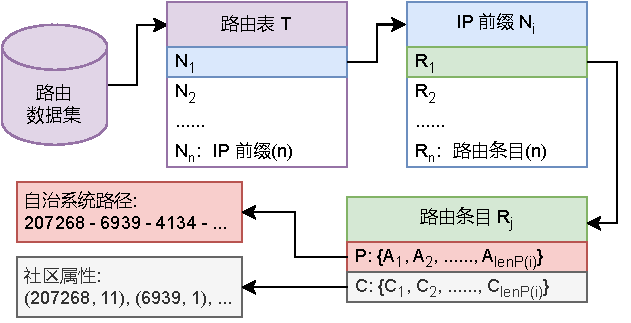
\includegraphics[width=0.7\linewidth]{chapter/c3_images/c3_data-struct.pdf}
    \caption{图网络路由数据集的组成结构,依层次为:路由数据集、路由表、网络前缀、路由及其包含的路径和社区属性}
    \label{c3_data-struct}
\end{figure}

\subsection{基于自治系统逻辑拓扑关系的图网络数据构建}

\subsubsection{层次结构分析}

\begin{figure}[h]
    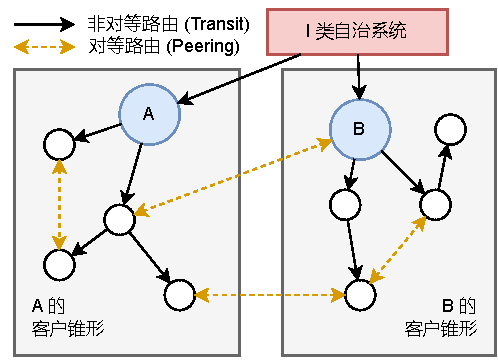
\includegraphics[width=0.6\linewidth]{chapter/c3_images/c3_dataset-layers.pdf}
    \caption{路由数据集的层次分解。由 A 和 B 建立的两个客户锥形之间存在的对等路由}
    \label{c3_dataset-layers}
\end{figure}

图 \ref{c3_as-distance} 的结果能够反映出,广域网络的一些连边事实上并不在路由信息的传递中扮演作用,这导致了完全通过网络路由数据集构建的图网络与真实路由系统的运作模式不一致,例如图中的平均自治系统长度的差异,而这些差异最终都将体现在模型的运行效果上。因而,为了实现下游模型训练效果的优化,需要从广域网络路由协议的角度去分析这些在路由过程中不扮演消息传递角色的路由,并将其从构造的图中去除。

通过对广域网路由模型的分析,广域网络的路由可以被抽象为一个类树状结构加上一些随机噪声连边,这种现象能够通过自治系统的互联模式很好的解释。如图 \ref{c3_dataset-layers} 所示,由于互联网络是由非对等互联路由和对等互联路由共同构成,前者具有一定的层次性,因而形成一种类树状结构;而后者则存在一定的无序性,因此能够随机地连接网络中的节点。由于对等路由仅仅在直接连接的自治系统之间交换路由,并不会传递其它自治系统的路由,因此这部分的路由在用于异常检测上时能够被移除而不影响异常检测的效果。

为了验证上述猜想,首先在图上定义对等路由:

对于一个路由表${R_i}$,某两个节点 $V_a$ 和 $V_b$ 的之间的路由$R_p$是自治系统长度为 1 的路由,假设其连边为 $E_p$,则它是对等(Peering)路由,当且仅当路由表${R_i}$的任意路由 $R_k$ 中不包含长度大于1,且路径末端为连边 $E_p$ 的自治系统路径。或者以公式\ref{peering_route}的方式表示:
\begin{equation} \label{peering_route}
R_p = \{P: \{E_p<V_a, V_b>\} \}, 
\forall R_k \in \{R_i\} \parallel len(P_k) \geq 1, E_p \neq last(P_k \in R_k)
\end{equation}

随后,为了研究现有数据集中的路由类型的分布状况,本研究使用了 RIPE RIS 和 DN42 在 2022年12月的数据集,对数据内节点介数中心度与它们的对等/非对等(Peering/Transit)路由的数量做出了统计和对比。实验结果如图 \ref{c3_route-centrality} 所示,可以从图中发现,互联网的非对等路由更具结构性,越具有中心度的节点,将具有越高的非对等路由,而对等路由则在大部分节点上呈现出随机的分布;作为对照,DN42 这类分布式网络由于大部分节点间完全通过双向非对等路由的形式进行路由交换,在路由数量与其介数中心度的关联上并没有互联网数据集密切。

\begin{figure}[h]
    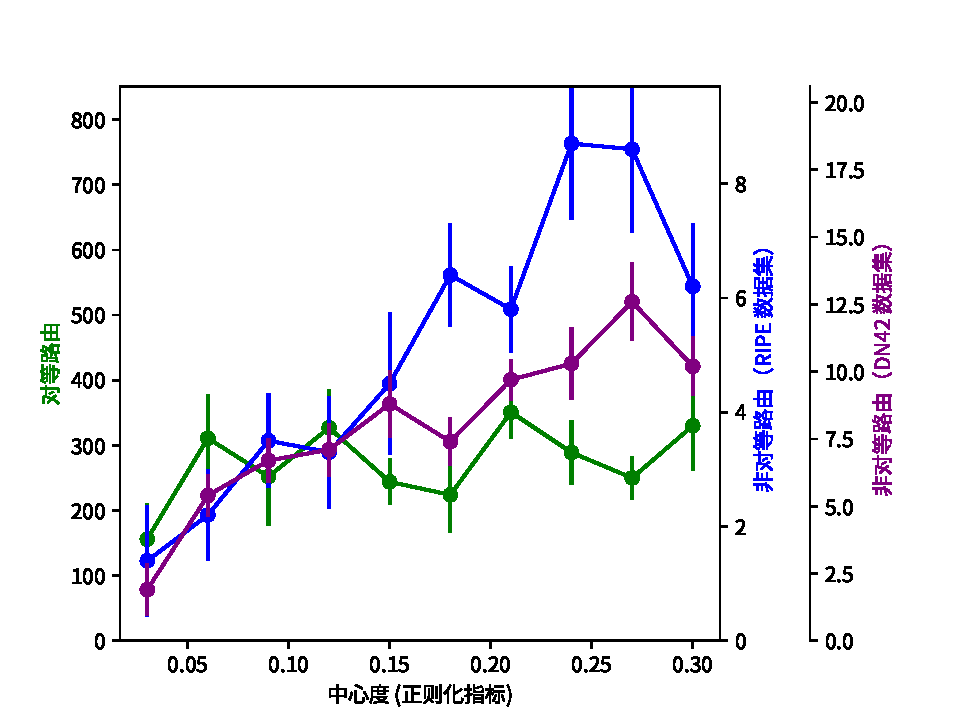
\includegraphics[width=0.9\linewidth]{chapter/c3_images/c3_route-centrality.pdf}
    \caption{路由数据集上对等/非对等(Peering/Transit)路由的数量与中心度的关联}
    \label{c3_route-centrality}
\end{figure}

假如去除路由系统中的对等连边,是否会有度为0的孤立节点产生是另一个因此出现的问题。根据路由条目沿非对等路由传播的定义,某个节点 $V_a$ 与 网络中任一节点互通,且并非通过对等方式互通(即 $d(V_a)\neq n-1$),则$V_a$与任一I类自治系统应当存在非对等路由关系,而根据I类自治系统的定义,没有任何节点向它们提供非对等路由,因此它必然存在一条通往I类自治系统的非对等路由。通过以上方式,能够证明,所有能够访问全部广域网的节点,要么与其余全部节点存在对等路由,要么存在至少一条可进入数据集的非对等路由。

% 对于自治系统节点 $V_a$,而言,设子图区域 $G_z = <\{V - V_a, E - E_a\}>$,其中 $E_a = \{ \forall E_k(V_{from}, V_{to}) \in E, if (V_{from} = V_a \parallel V_{to} = V_a ) \}$。假设 $V_a$ 不存在 Transit 路由,对于 $V_a$ 的临接节点集 $V_{nei}$,一定存在 $V_{nei} \leftrightarrow V_a $,即路由双向可达,由于 Peering 路由长度一定为 1,则对于 $V_a$ 的非临接节点集 $V - V_{nei}$ 一定在 $G_z$ 上存在一条通向 $V_a$ 的 Transit 路由,为了保证 $V_a$ 一定在 $V_{sample} \in V - V_a \in G_z$ 为起点的采样数据集中出现,即 $E\{P(V_a \rightarrow V_{sample})\} = 1$,要么 $V_{nei} =V - V_a$,要么 $V_a$ 存在至少一条 Transit 路由。

事实上,上述区域 $G_z$ 被称为DFZ(Default-Free Zone)区域,其被定义为拥有全部广域网路由的自治系统路由器集合。即使对等路由在实际网络中存在流量交换的意义,在此场景下仍然能够将其去除从而不影响图网络整体在异常检测上表现出的结构性。

\subsubsection{图生成算法}

在验证了上述假设的条件下,对路由数据的处理问题转化为了如何在现有的数据中提取并去除对等路由。

在此基础上,路由数据集的图生成算法定义如表 \ref{algo-datagen-topo} 所示。该算法能够通过上述方法去除没有对异常检测存在意义的对等互联路径,从而输出一张更具结构性特征的广域网路由拓扑图,从而达到降低网络复杂度、稠密度的效果。

\begin{algorithm}[H]
    \KwData{输入路由集合 \{$R_i$\} 和预先定义的I类ISP 表 $V_{t1}$}
    \KwResult{输出一份由此数据生成的数据集}
    初始化图网络:
    $G<V=\{\},E=\{\}>$\;
    提取路由路径:
    $\{P_i \in R_i\}$\;
    初始图网络生成:
    \For{$\{V_a, E_{ab}, V_b\} \in P_i$}{
    $G<V+=\{V_a, V_b\},E+={E_{ab}}>$
    }
    \For{每个非I类自治系统的节点$V_i \notin V_{t1}$,检查它们的连接 $e_i$:}{
        \If{$e_i$ 满足对等路由的条件}{
            从图中删除它: $G<V, E=E-e_i>$
        }
    }
    输出网络 $G$\;
    \caption{基于逻辑拓扑关系的路由图网络生成算法}
    \label{algo-datagen-topo}
\end{algorithm}

\subsection{基于自治系统路由相似度度量的图网络数据构建}

除了直接使用数据集中的路由数据进行图的拓扑构建外,还能使用原数据的节点相似度度量对图进行构建。这是对于过于冗余的原数据集的另一种利用方法,该方法将其转换为节点间路由度量的带权图,这能够将原本的路由拓扑图变得稀疏化,同时将冗余数据转化为正则化的指标。

虽然介数中心度在反映路由中心度上更具优势,但它的计算复杂度在面对互联网数据集的规模(>5000万条连边)的情况下过高,而在图网络中,基于余弦相似度的节点表征方法相比而言更加实际,它通过采样节点的邻居信息并实现对节点之间的相似度度量,并更加快速,适合使用在数据集的处理上。它的定义如公式 \ref{cos_dist} 所示。
\begin{equation} \label{cos_dist}
d_{cos}(V_A,V_B) = \frac{\Sigma_{nei} V_i^A V_i^B}{\sqrt{\Sigma_{nei} (V_i^A)^2} \sqrt{\Sigma_{nei} (V_i^B)^2}}
\end{equation}
% 公式

根据上述定义,使用以下算法利用相似度度量对原始数据集进行处理:

% 构图算法表格

\begin{algorithm}[H]
    \KwData{输入路由集合 $\{R_i\}$}
    \KwResult{输出一份由此数据生成的数据集}
    初始化图网络:
    $G<V=\{\},E=\{\}>$\;
    \For{每条路径 $\{P_i \in R_i\}$}{
        \For{路径上的相邻两个自治系统 $(V_a, V_b) \in P_i$}{
            对边赋权重:$e(V_a, V_b) += d_{cos}(V_a, V_b)$
        }
    }
    \For{图 $G$ 中的每个顶点 $\{V_i \in V \in G\}$}{
        \For{顶点上的每条边 $(V_a, V_b) \in E(V_i)$}{
            \eIf{进行 top-k 计算:$topk(E(V_a, V_b))$}{
                保留边 $E(V_a, V_b)$ \;
            }
            {
                删除边 $E(V_a, V_b)$ \;
            }
        }
    }
    输出网络 $G$\;
    \caption{基于路由相似度度量的路由图网络生成算法}
    \label{algo-datagen-sim}
\end{algorithm}

如表 \ref{algo-datagen-sim} 所示的算法描述,在获取数据集后,对路径上每一对自治系统节点间的相似度进行余弦相似度计算,将其作为邻接矩阵的权值。对于生成的临接矩阵,它是一个全连接的完全图,使用每节点 topk 权值的平均值作为分界值,从而将其变为更加稀疏的图网络。

\section{实验及分析}
% 4-5 页

在本章节的实验环节,首先需要比较的是输入的数据集在参数规模上的横向差异,这对后续异常检测任务的效果差异的分析上具有作用;其次,由于本章所述方法是对数据集中图网络结构的变换,本文还将针对此方法输入和输出图网络的参数进行纵向对比,以初步分析所述方法在去除冗余边集和降低邻接矩阵稠密度上的效果。

在数字特征上反映出的优化效果仅反映在时间维度上,因而本文在接下来的对比实验中,采用了多种基于不同方法的模型以评估图网络生成算法在异常检测任务中的提升效果,从而评估算法在何种程度上保持和聚合数据集中原有拓扑特征;随后在案例分析中,本研究通过仿真的实验环境评估了两种方法在改善模型检测效果上的提升。

\subsection{数据集概述}

对于本章节提出的模型而言,它的性能不仅取决于是否能够在具有较强结构化拓扑特征的互联网数据集上取得良好的效果,还应当考虑其横向泛化特性,即是否能够适用于并不明显具有结构化拓扑特征的网络。先前章节提到了 DN42 是一类分布式网络,它相比由 IANA 管理的网络而言更具松散的结构而具有更少的层次性,适合用于本章节的实验部分。

在模型参数分析部分,由于未涉及到预设的异常参考值,本文采用了最近的来自两个分布式网络的路由数据,它们分别是采用了来自 RIPE RIS 的三个较近时间点的数据集和来自 DN42 的一个较近时间点的数据集,均采用 MRT 格式。相应的数据统计信息如表格 \ref{c3_data_input} 所示。

\begin{table}
    \caption{作为输入的路由数据集的统计信息}
    \begin{tabular}{lcccccccc}
        \toprule
        指标/数据集 & RIPE.2022.10 & RIPE.2022.11 & RIPE.2022.12 & DN42.2022.12 \\
        \midrule
        路由总数   & 10,068,040   & 10,072,615   & 10,165,549   & 82,664       \\
        前缀总数   & 103,162      & 104,265      & 104,523      & 716          \\
        \midrule
        节点总数   & 75,105       & 75,363       & 75,442       & 557          \\
        连边总数   & 2,228,343    & 2,230,203    & 2,246,004    & 2,756        \\
        \bottomrule
    \end{tabular}
    \label{c3_data_input}
\end{table}

在后续参数的使用上,对于基于相似度的构图方法的 k 值,本文从基于逻辑拓扑关系的构图结果中获取图网络的平均度数作为对应的值,具体的来讲,对于 RIPE 的几个数据集,它们的值为 4.35,对于 DN42 的数据集而言,它的值为 9.62,与基于 RIPE RIS 和 DN42 原始数据的估计是相近的。

% 数据量,表格 

\subsection{参数分析}

图网络参数是一个需要被首先考虑的问题,本文通过对上述三组来自 RIPE RIS 数据的输出连边数量及下降比例分析,总结出如表 \ref{c3_data_arg} 所示的结果。

从表 \ref{c3_data_arg} 中基于拓扑的模型的统计数据可以发现,该方法在对降低具有较多对等路由的网络连边数量具有较大的作用,这是该方法的原理所决定的,对于 RIPE 数据集而言,模型最大能够降低约 17\% 的无效连边数,其数量级约为 $10^6$ 左右,这在基于消息传递的多层图网络模型的嵌入效果和计算复杂度上会反映为较大的差异。

在 DN42 分布式网络数据集上,基于拓扑结构的构图算法并不能够取得与互联网数据集一致的边集优化效果,这一点可以从先前章节对 DN42 网络结构的概述中得到解释:具有实验性质的网络通常不具备较高的层次性,因而也存在较少的对等路由,对于此种广域网络系统上的路由异常检测需要更好的优化方案。

在基于相似度的图生成模型上,由于设定的参数 k 对边集大小具有控制作用,因而此处的数值对比意义不大,仅反映对应 k 值在路由数据集上的对应结果规模。在异常检测模型的实际运行中,需要兼顾计算效率和运算性能以确定最优的 k 值。

\begin{table}
    \caption{输入与输出的图网络参数对比}
    \begin{tabular}{llcccccccc}
        \toprule
        算法                     & 指标/数据集 & RIPE.2022.10 & RIPE.2022.11 & RIPE.2022.12 & DN42.2022.12 \\
        \midrule
        \multirow{2}{*}{基于拓扑}  & 输出连边 & 1,847,296    & 1,857,759    & 1,866,429    & 2,552        \\
                               & 下降比率   & 17.1\%       & 16.7\%       & 16.9\%       & 7.4\%        \\
        \midrule
        \multirow{2}{*}{基于相似度} & 输出连边 & 2,092,414    & 2,065,167    & 2,091,029    & 2,599        \\
                               & 下降比率   & 6.1\%        & 7.4\%        & 6.9\%        & 5.7\%        \\
        \bottomrule
    \end{tabular}
    \label{c3_data_arg}
\end{table}

\subsection{对比实验}

\subsubsection{分析指标}

% 跑一个模型,随机选取一系列路径,看对同一个新增路径数据的前后结果是否在同一个 rank 上。
为了检验数据集是否在拓扑特征上与处理前一致,本章节将已知的网络路由异常数据集提供给多个无监督的图嵌入模型,并分析在路由异常事件间的异常路由检出的准确度和 F1 值。具体地,本实验选择了 HOPE,DeepWalk,GraphSAGE 三种图网络嵌入的基线算法进行衡量,以标准化误差 0.5 作为异常阈值。

在数据集的选取上,对比实验选择了 RIPE RIS 于 2010、2017、2022 三个时间段上具有已知异常路由异常标记的数据集,使用异常发生前一天作为基准数据训练模型,并将路由异常开始后的流式路由更新输入到模型以获取路由异常检测的输出值作为对比。

\subsubsection{实验结果}

此实验采用了上述基线模型来评估图生成算法降低冗余和无效连边的性能,表 \ref{c3_s3tab} 报告了在不同模型下的异常检测结果,从中可以得到下列的发现:

\begin{enumerate}
    \item 相比于原始数据而言,基于拓扑和基于相似度的图构建方法与各基线模型的配合在大部分场景下能够取得异常检测结果的改善,这意味着本章所提出的模型达到了预期的效果。
    \item 基于拓扑的构图模型在总体上优于本实验中设定数值的基于相似度的构图模型,本研究将其归结于两种原因:
          \begin{enumerate}
              \item 其一是尽管基于相似度的构图方法能够通过对节点特征相似度的 topk 的方式降低原始数据在图上的稠密度,但它实质上并没有在根本上移除无效边集,因而在输出的图网络中引入了噪声。
              \item 其二是基于相似度的构图方法的效果完全依赖于 top-k 中确定的 k 值,而对于原始数据实际组成的图网络而言,节点的连边数量将会根据节点的重要程度产生不同的权重。
          \end{enumerate}
    \item 对于基于拓扑的图构建方法而言,总体上各异常检测模型在更具结构化、邻接节点和路由关系更加复杂的互联网路由数据集(RIPE 数据集)能够取得更好的效果,这是符合本研究的参数分析章节的预期的结果。
    \item 基于相似度的构图模型上在使用类似 DN42 的分布式网络数据集上存在性能不佳的问题,其中的一种可能原因是,管理松散、相互连接从而具有较少层次结构的分布式网络的节点之间的相似度距离会更加接近。
\end{enumerate}

\begin{table}
    \caption{对比实验结果}
    \begin{tabular}{lcccccccc}
        \toprule
                        & \multicolumn{2}{l}{RIPE.2010} & \multicolumn{2}{l}{RIPE.2017} & \multicolumn{2}{l}{RIPE.2022} & \multicolumn{2}{l}{DN42.2022}                                                                     \\ \cmidrule(lr){2-3} \cmidrule(lr){4-5} \cmidrule(lr){6-7} \cmidrule(lr){8-9}
        模型              & Acc.                          & F-1                           & Acc.                          & F-1                           & Acc.           & F-1            & Acc.           & F-1            \\ \midrule
        原始数据                                                                                                                                                                                                                \\
        \quad HOPE      & 0.712                         & 0.698                         & 0.708                         & 0.682                         & 0.709          & 0.688          & 0.692          & 0.671          \\
        \quad DeepWalk  & 0.768                         & 0.770                         & 0.754                         & 0.741                         & 0.750          & 0.757          & 0.751          & 0.755          \\
        \quad GraphSAGE & 0.793                         & 0.820                         & 0.815                         & 0.808                         & 0.784          & 0.814          & 0.807          & 0.801          \\ \midrule
        基于拓扑的构图模型                                                                                                                                                                                                           \\
        \quad HOPE      & 0.761                         & 0.754                         & 0.734                         & 0.721                         & 0.770          & 0.724          & 0.748          & 0.727          \\
        \quad DeepWalk  & 0.794                         & 0.784                         & 0.791                         & 0.786                         & 0.809          & 0.802          & 0.771          & 0.776          \\
        \quad GraphSAGE & \textbf{0.835}                & 0.824                         & \textbf{0.843}                & \textbf{0.821}                & \textbf{0.830} & \textbf{0.840} & \textbf{0.809} & \textbf{0.813} \\ \midrule
        基于相似度的构图模型                                                                                                                                                                                                          \\
        \quad HOPE      & 0.705                         & 0.703                         & 0.721                         & 0.715                         & 0.722          & 0.711          & 0.682          & 0.673
        \\
        \quad DeepWalk  & 0.780                         & 0.767                         & 0.778                         & 0.760                         & 0.762          & 0.752          & 0.759          & 0.770          \\
        \quad GraphSAGE & 0.823                         & \textbf{0.830}                & 0.820                         & 0.810                         & 0.812          & 0.826          & 0.801          & 0.807
        \\
        \bottomrule
    \end{tabular}
    \label{c3_s3tab}
\end{table}

\subsection{案例分析}

\subsubsection{实验方法}

为了确定模型性能的改善是由于图构建时采用的算法,本章基于 DN42 平台构建了仿真的测试环境,试图通过案例分析的方式确定算法的有效性。

如图 \ref{c3_case-flow} 所示,作为实验环境的初始化,节点 A(AS4242421331) 被接入到 DN42 网络中,并将其与 B(AS4201271332) 构成对等路由关系,其中 C(AS4242421331) 是 A 和 B 的共同 Transit 提供者,这是一个用于验证本章所述算法正确性的最小可操作场景。通过节点 A 向 DN42 的路由收集器发起路由反馈会话,并维持正常的网络路由一段时间,正常的路由表能够被 GRC 收集并生成数据集文件。

在随后的实验步骤中,节点 A 通过更长前缀的方式劫持节点 B 的路由,意图将通往该网络的流量劫持至节点 A 所控制的网络中。该行为将被网络自身及其各阶邻居通告给 GRC,随后 GRC 将以更新文件的形式将包含异常路由的路由表生成出来。

\begin{figure}[h]
    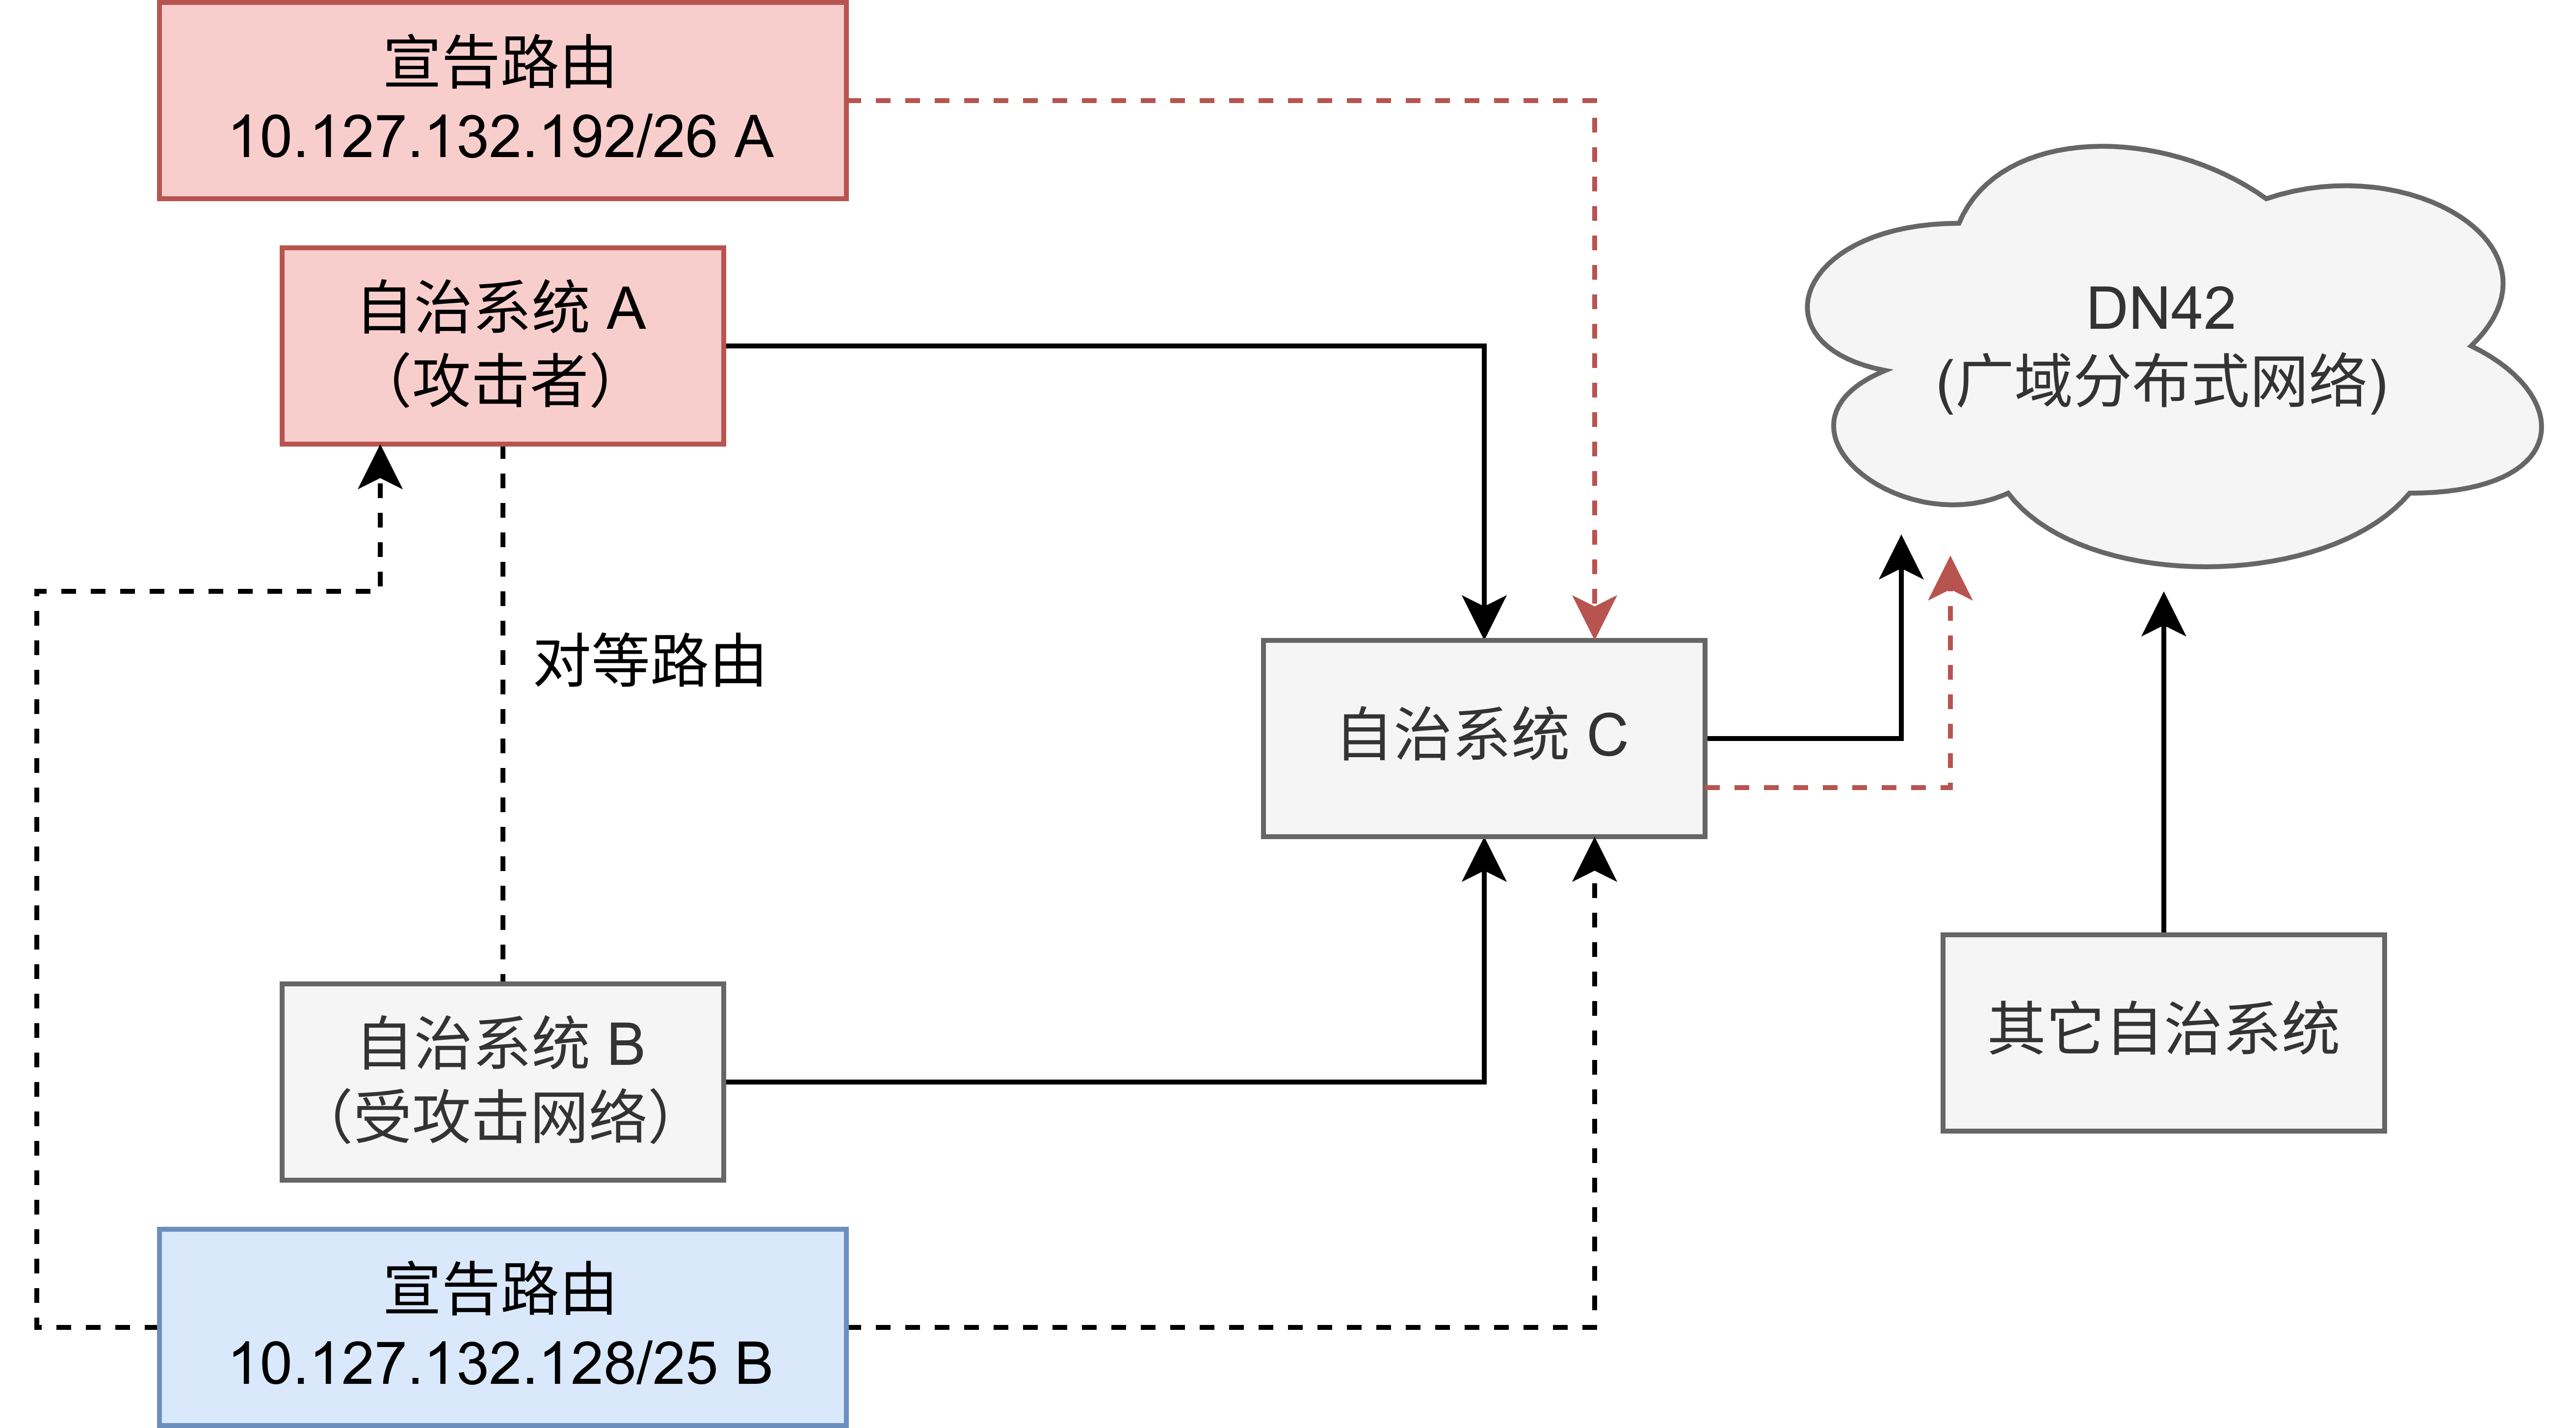
\includegraphics[width=0.7\linewidth]{chapter/c3_images/c3_case_flow.png}
    \caption{案例分析实验流程}
    \label{c3_case-flow}
\end{figure}

上述模型将以这两个文件作为输入,使用 GraphSAGE 算法模型进行嵌入并输出异常分数,从而判断本章所提出的算法对无效和冗余路由的去除效果,及对嵌入结果的影响。由于在此实验中,异常路由是已知的,因而可以从数据集中获取所有包含异常的路由样本,并将其送入模型进行异常检测。

基于对比实验的效果及在图构建算法设计上的规则,预期的结果是,使用原有数据集构成的路径的模型将在所有异常样本中取得相对更低的分数,而使用基于结构特征的构图方式的模型将在所有样本中取得相对更高的分数在,这是由于如图 \ref{c3_case-flow} 所示,在不去除自治系统 A 和自治系统 B 之间的对等路由的状况下,由原数据产生的图网络将包含 A、B 之间的连边,从而将 A、B 两个节点间的嵌入相似度拉近,进而影响到异常检测的分数。

\subsubsection{实验结果}

对于基于两种构图方式的所有异常路由样本的异常分数输出如图 \ref{c3_case-score} 所示。可见两种模型在异常样本的输出上与预期基本符合,与原始数据集相比在相同模型的分数输出上均具有提升。其中,基于结构特征的构图方式总体上对异常路由的预测效果提升最大(异常分数提升约 30\%),这反映出了基于结构特征的构图方式达到了相对而言更好的去除冗余路由的效果,而基于相似度的构图方式也相对于完全使用原始数据构图的方法在异常检测分数上提高了约 18\%,此结果展现出了,即使在不去除原始拓扑中的冗余路由的情况下,适当降低输入图网络的邻接矩阵稠密度同样能够改善模型的检测效果。

\begin{figure}[h]
    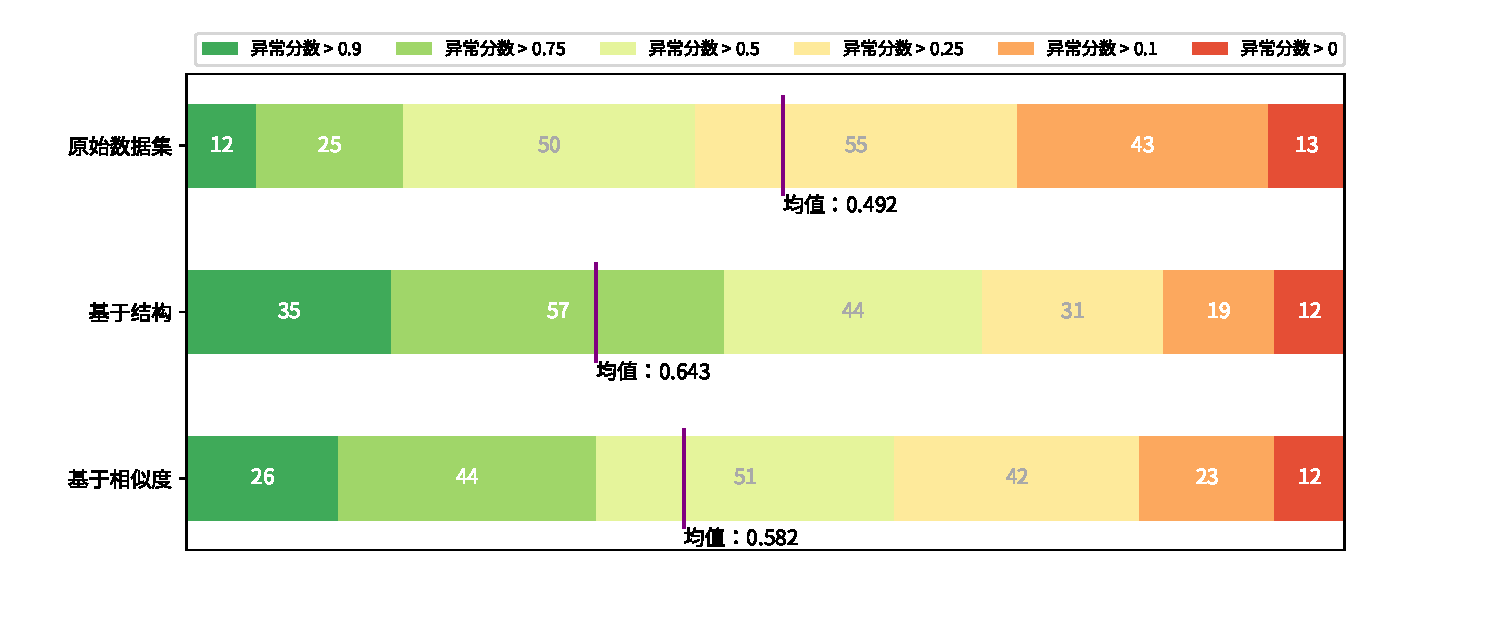
\includegraphics[width=\linewidth]{chapter/c3_images/c3_case-score.pdf}
    \caption{两种模型在异常路由样本下的输出分数}
    \label{c3_case-score}
\end{figure}

\section{本章小结}

本章主要针对海量路由数据集提出了一种图数据生成算法。在 3.1 节,介绍了现有的广域网路由数据集,并分析了其中存在的问题及对图网络模型的影响。在 3.2 节,本文通过分析广域网络的拓扑结构特征,将路由数据集中的噪声通过一种基于客户锥形的方法分离出来,并设计出了两种不同方式的图生成算法框架。在 2.3 节,为了实证数据集的有效性,通过节点相似度和嵌入相似度的比较,本文使用一些常见的基线模型在该算法生成的数据集中进行了实验分析。
\chapter{基于属性信息聚合的广域网络路由异常检测研究}

在先前章节的实验中,传统的图卷积网络在广域网数据集中展现出计算复杂度过高的问题,并存在对未知节点的泛化能力的不足的缺陷。本章节将从基于信息聚合的图网络算法入手,以 GraphSAGE 为基本框架,将数据集包含的路由特征的拓展到该模型中。

% 15 页
% 魔改 GraphSAGE
% https://toutiao.io/posts/ydj46sp/preview

\section{研究背景}

% 1.5 页

近年来,随着卷积神经网络的发展,一些研究注意到了卷积在传统的基于图像的领域具有提取局部特征的良好特性,而基于图卷积模型的出现更是将卷积的思想带入了图网络领域:利用结合相邻节点的信息和自身信息的方式,能够得到图网络自身的局部表示\citing{scarselli2008graph}。基于以上思想,将图卷积运用在广域网络的路由数据中一种可行的方案。

然而,图卷积网络自身的运算量非常巨大,在具有大量节点的数据集上对于一个多层的图卷积网络的临接矩阵做卷积操作,在实际场景中很有可能超出可行的运算能力。此外,图模型中基于 GNN 的架构,例如 Deep Walk 和 GCN 等模型,通常需要在数据发生更新的时候对整个图进行重新学习,由于本研究涉及到的路由数据集所包含的图结构过于庞大,而异常检测的任务决定了模型需要一段时间后进行重新训练,这将严重阻碍模型在实际生产环境中的工作效率\citing{hamilton2017inductive}。

因而一种称为 GraphSAGE 的基于邻接节点采样的方法\citing{hamilton2017inductive}被提出。它通过预先对节点的邻居进行采样,从而降低了后续特征聚合获得嵌入需要处理的节点数量,另外,该模型的参数量是受参数控制且恒定的,不会随着图网络规模的增加而不断扩张,这使得该模型在应对路由条目不断增长的互联网路由表上具有一定优势。

然而,GraphSAGE 模型的邻居聚合一般使用基于均值的函数,没有考虑到不同的邻居节点应当对特征具有不同的贡献,该模型在采样阶段和损失的计算上也存在类似的问题,一项研究指出,对于具有一定路径拓扑的路由网络的场景而言,使用这样的计算方式并不合适\citing{el2022deep}。因此,如何设计聚合模型以针对性地学习与路径相关的特征,是一个值得探讨的研究话题。

为此,本章从经典的 GraphSAGE 模型出发,根据实际场景对该模型的采样方法、聚合函数、损失函数等关键模块进行了分析,并据此提出了对应的基于路由生成的图结构的路径特征的表示方法,这种方法利用路径信息对算法中的各组成部分赋予不同的权重,相比于典型的 GraphSAGE 模型能够反映出路径所导致的邻居节点间的不同,从而达到提升异常检测模型准确性的目的。

综上所述,本章节提出的模型贡献如下:

\begin{enumerate}
    \item 将属性信息聚合的图网络算法应用在网络路由的图数据集上,降低了图网络算法的计算开销,并使得模型在生产环境中的高效更新成为了可能。
    \item 设计了一种针对网络路由的图结构的邻居特征聚合算法和对应的损失函数,能够有效地利用数据集中的路径特征。
    \item 设计了一种根据路径信息采样邻居特征的邻居采样算法,从而更有效地从原始图网络中采样获得更具代表性的子图。
\end{enumerate}


\section{模型设计及实现}

\subsection{模型结构}

\begin{figure}[h]
    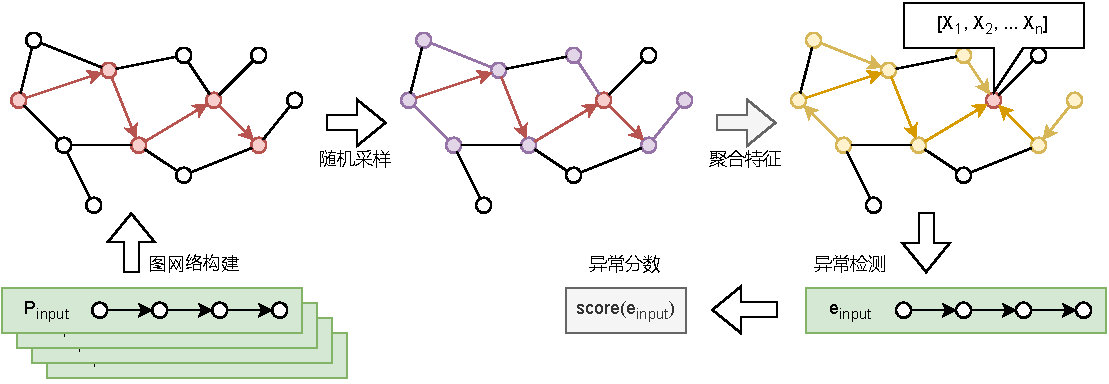
\includegraphics[width=\linewidth]{chapter/c4_images/c4_model.pdf}
    \caption{模型结构图}
    \label{c4_model}
\end{figure}

这一节的模型架构将以 GraphSAGE 模型为基础,通过对它的三个重要部分进行探讨,并针对广域网络的路由数据的特点,本研究从路径的角度出发分别提出对应的利用数据集中路径信息的方法。

如图 \ref{c4_model} 所示,本章提出的模型的结构包括了随机采样、聚合特征、异常检测三个部分,它的输入是一套网络路由数据集,首先输出对应数据集在图上的嵌入,最后通过异常检测输出对路由系统中路径更新的异常分数。

\begin{enumerate}
    \item 随机采样:该部分通过已知的路径信息优化随机采样的概率,从而实现有权重且权重基于路径信息的随机采样。
    \item 聚合特征:该部分通过引入路径带来的差异,对邻居间信息的聚合方式进行了调整,实现了基于路径权重的邻居聚合。
    \item 异常检测:该部分通过前序模型获得的嵌入,对比新路径的嵌入从而进行异常检测。
\end{enumerate}

\subsection{模型分析}

本文选取 GraphSAGE 作为模型的框架,是由于它具有以下特性:

\begin{enumerate}
    \item 训练数据通过采样获得。传统的图神经网络在面对网络路由等大规模的数据集上普遍存在性能不足的问题,GraphSAGE 通过采样子图的方式减小了需要计算的图网络矩阵尺寸,从而减少了性能开销。
    \item 聚合和采样函数具备调整空间。GraphSAGE 模型在框架上仅规定了前向传播的方法,具体的聚合和采样函数是模块化的,能够在节点层面上进行调整,这使得将路径因素引入到模型中是可行的。
\end{enumerate}

然而,GraphSAGE 模型非常依赖采样函数、聚合函数、损失函数的选取,在传统的 GraphSAGE 模型中路径是不存在的,这些函数仅会引入了节点连边的拓扑差异,在上述函数中直接采用现有方法不能利用数据集中的路径特征。因此,为了能够在路由数据集上针对性地提取特征,模型应当在这三个重要部分中体现出相应的权重差异,本研究通过在算法中引入路径因素,分别为三个部分设计了对应的改进方法。

\subsection{基于节点权重的随机采样}

大部分图网络中,图中的每个节点的度值是不一致的,为了提高模型性能,GraphSAGE 模型对于一般的图网络的通用做法\citing{hamilton2017inductive} 是为每个节点采样固定数量的邻居。而基于广域网络路由架构的性质而言,即使是在分布式网络中,广域网路由系统中的自治系统会在网络中对路由有着不同程度的控制力,即它们应当从/向不同尺度的节点获取/传递特征。

在图网络中,对节点在图网络中的控制力强度的度量方法通常是中心度,而对于在路由系统的嵌入任务而言,其中的介数中心度相比之下更具有统计意义,该方法能够将节点在最短路径中出现的频次,即介数中心度作为采样指标,从而在一定程度上反映自治系统对临接节点路由的控制能力,而这种控制能力的度量在实际场景中即对应其路由异常传播的规模。

为了验证这一结论,本研究针对节点的介数中心度的分布状况进行了实验分析。实验对来自 2022 年 10,11,12 三个月份的 RIPE RIS 数据样本按照第三章所述的基于拓扑的构图方式进行了图网络生成,以便排除对等路由的影响,随后对每一个自治系统计算了其对应的介数中心度,详细的统计结果如图 \ref{c4_node-centrality} 所示,为方便展示,横坐标轴已修改为通过对数的方式呈现。

\begin{figure}[h]
    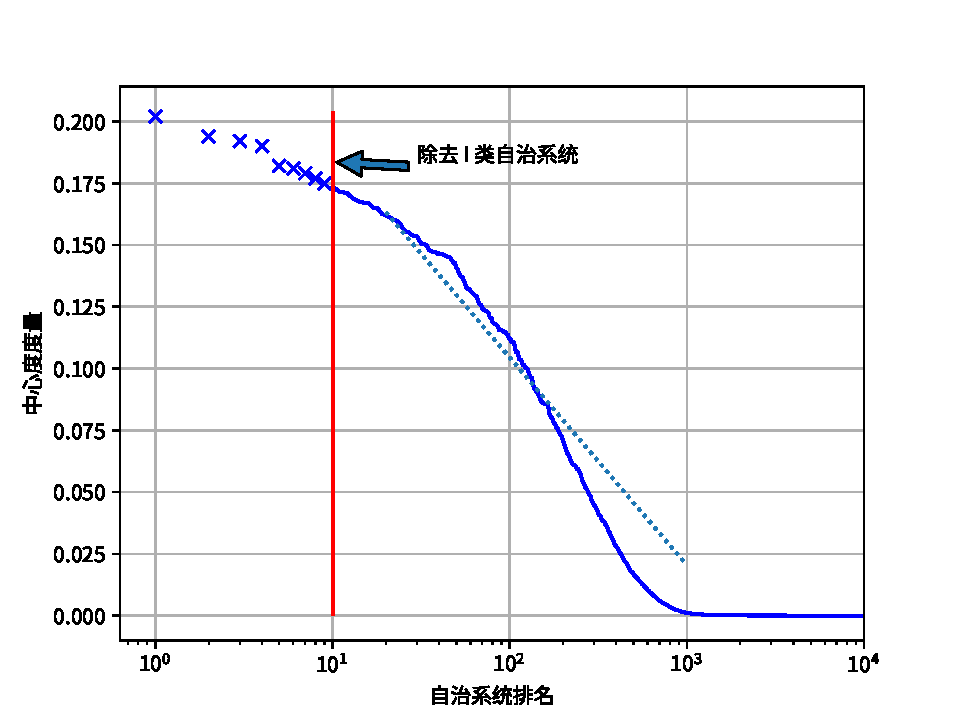
\includegraphics[width=0.8\linewidth]{chapter/c4_images/c4_node-centrality.pdf}
    \caption{RIPE 数据集中的介数中心度的分布状况}
    \label{c4_node-centrality}
\end{figure}

图 \ref{c4_node-centrality} 的结果可以反映出自治系统在中心度上的分布情况,由于 I 类自治系统自身根据定义具有很高的中心度,在去除了互联网所有 I 类自治系统(图中的红线部分右侧)后的图表趋势大致上在对数范围呈现线性下降的趋势(图中的蓝色虚线部分)。因而可以认为基于介数中心度的指标对节点进行采样和后续的特征聚合是可靠的。

因此,本章提出了如公式\ref{s3_sample_model}所示的采样模型:
\begin{equation} \label{s3_sample_model}
P_b(a) = \Sigma_{b, (a,b) \in E} \frac{\omega(a,b)}{\Sigma_{a} \omega(a,b)}, \omega(a,b) = 1 + \theta_{sample} \cdot \frac{N_{paths}^a(b)}{N_{paths}^a}
\end{equation}

其中 $\theta_{sample}$ 是一种权重值,通过它能够调整采样邻居数与其中心度的关联,当此值为 0 时,该模型退化至普通的固定采样模型。$N_{paths}^a(b)$ 是全部经由 a 节点的路径中同时经由 b 的路径数量,模型通过该式使得具有更多路径关联的邻居具有更大的采样概率。通过在原图网络上的 k 次迭代采样能够获得一个用于 k 层邻居聚合模型的子图。同时,为了限定采样规模,该采样过程由一个参数 $N_{sample}$ 控制,并决定对于一个节点而言的采样邻居数量。

根据此模型,在对邻居进行采样时将考虑到与邻居的共同路径比例,即更容易采样到具有更多公共路径的邻居信息。

\subsection{基于路由特征的邻居聚合}

一般而言,在 GraphSAGE 模型中一般使用均值聚合器方案\citing{hamilton2017inductive},即对相邻节点和本节点的上一层输出取均值,并据此进行线性变换,进而产生当前层的输出。具体的实现方式见公式\ref{graphsage_default_aggr}。
\begin{equation} \label{graphsage_default_aggr}
h^k_v \leftarrow \sigma(W \cdot MEAN(\{h_v^{k-1}\}\cup \{h^{k-1}_u, \forall u \in N(v)\}))
\end{equation}

在一般的图网络中,它能够对图节点的邻居特征起到很好的聚合效果。然而对于当前场景下的节点特征,由于存在路由路径相关的因素,对于一个自治系统即一个节点而言,它的相邻节点提供的路由路径是不一样的,聚合函数使用完全的均值函数将抹去邻居间由路径产生的的差异,从而没有利用上数据集中存在的路由特征。

为了聚合包含路径特征的相邻节点信息,本研究引入了一种新的聚合函数,定义如式\ref{graphsage_model_aggr}所示,它通过与路径相关的参数 $p(u)$ 控制的权重对邻居特征进行基于路径的聚合。
\begin{equation} \label{graphsage_model_aggr}
h^k_v \leftarrow \sigma(W \cdot MEAN(\{h_v^{k-1}\} \cup \{E\{p(u) \cdot h^{k-1}_u\}, \forall u \in N(v)\}))
\end{equation}

由于对相邻节点的相关统计量的操作均被包含在均值函数以内,它自身也具有类似均值聚合函数的结构,因而它满足聚合函数的对称性条件,即它能够确保模型能够被基于梯度的方式训练,并被应用在以任何可能顺序排列的临接节点的集合上。

根据以上的邻居聚合模型,一般的基于均值的聚合函数被加权平均的聚合函数替代,其中权值为经由路由更多的邻居节点。例如在如图 \ref{c4_nei-agg} 所示的采样子图中,传统的 GraphSAGE 模型没有考虑数据集的路径特征,在进行聚合时思路通常是对节点 $V_i$ 的所有邻居 $V_{nei}$ 及其高阶邻居赋予同样的权重进行求均值的处理;而在本模型中,由于存在路径的影响,节点 $V_i$ 在进行节点聚合时,将会相比于邻居节点 $V_b$ 和 $V_e$ 更多考虑来自邻居节点 $V_a$ 包含的特征信息,因为它们共享更多的与 $V_i$ 相关联的路由路径,这里也体现了本方法中基于路径特征的特点。

\begin{figure}[h]
    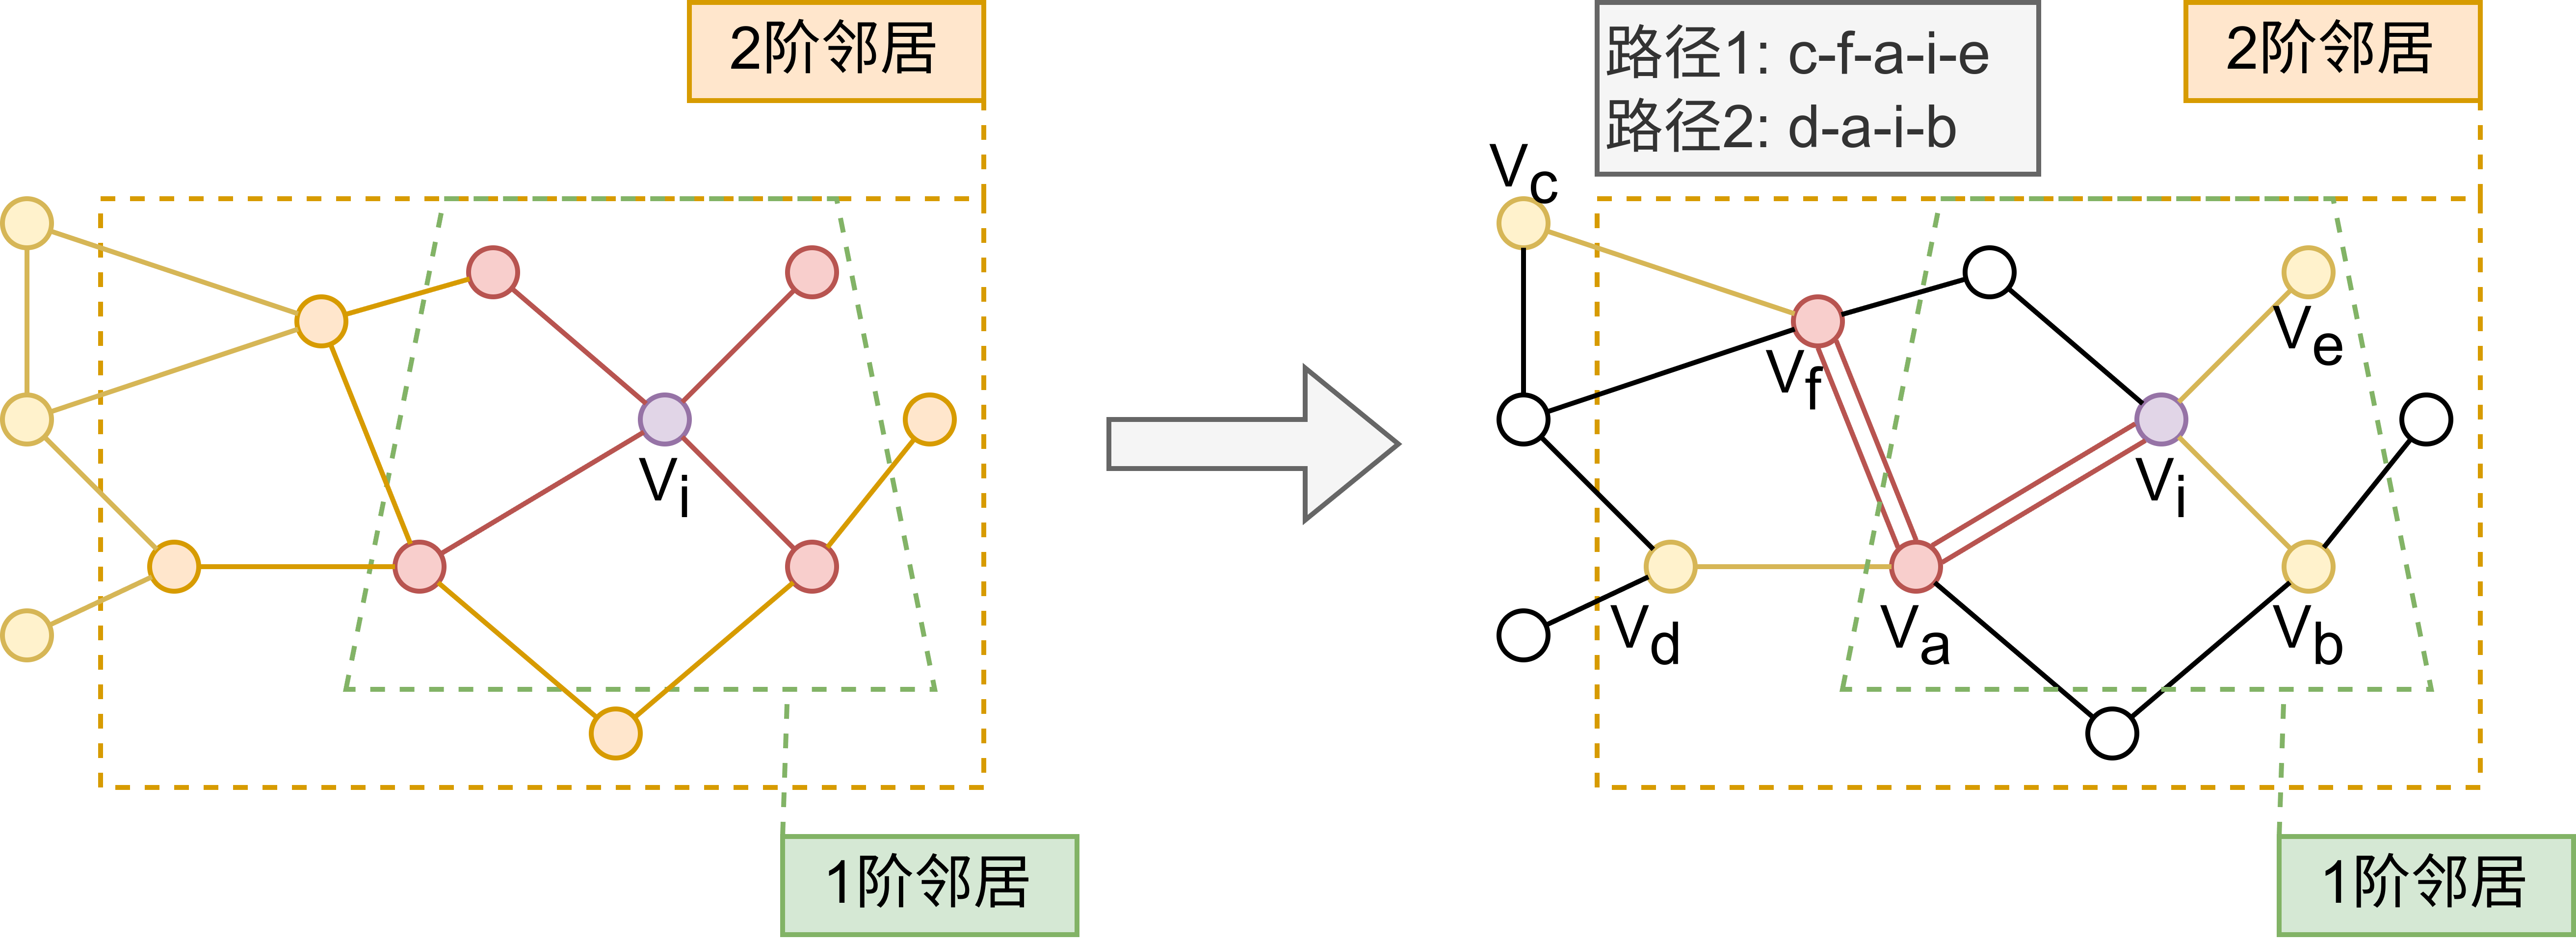
\includegraphics[width=0.9\linewidth]{chapter/c4_images/c4_nei-agg.png}
    \caption{邻居聚合方式的对比}
    \label{c4_nei-agg}
\end{figure}

\subsection{基于路由特征的损失设定}

基于与上一节相同的原理,本研究需要对基于图的无监督损失函数进行修正,它的原始定义如公式\ref{graphsage_default_loss}所示。
\begin{equation} \label{graphsage_default_loss}
J_G(Z_u) = -log(\sigma(z_u^{T}z_v)) - Q \cdot E_{v_n \sim P_n(v)}log(\sigma(-z_u^{T}z_v))
\end{equation}

它从当前节点的临接节点中采样对数损失,而从非临接节点中采样负的对数损失。该函数在 GraphSAGE 模型中被提出\citing{hamilton2017inductive},并被解释为一种实现在嵌入结果中相似嵌入节点更加接近的方法。

在本研究所述模型中,通过上述方式进行无监督的损失计算同样将抹去邻居间由路径产生的的差异,因而需要进行调整以适应存在路径特征的情形。

利用与上一节构造基于路径的聚合函数的方法可以设计一种损失函数,使得它能够可控地使得在同一条路径上的节点嵌入存在相似性,它的实现方式具体如公式\ref{graphsage_model_loss1}与公式\ref{graphsage_model_loss2}所示。
\begin{equation} \label{graphsage_model_loss1}
J(Z_u) = J_G(Z_u) + \theta_{loss} J_P(Z_u)
\end{equation}
\begin{equation} \label{graphsage_model_loss2}
J_P(Z_u) = -Q \cdot E_{v_n \sim P_{inpath}(v)}log(\sigma(z_u^{T}z_v)) -Q \cdot E_{v_n \sim P_{\sim inpath}(v)}log(\sigma(-z_u^{T}z_v))
\end{equation}

其中 $E_{v_n \sim P_{inpath}(v)}$ 表示在同一路径上的节点,即通过路径关联的节点;而 $E_{v_n \sim P_{\sim inpath}(v)}$ 表示不在同一路径上的节点,即互不通过路径关联的节点。

该损失公式通过结合图网络拓扑上的邻居损失 $J_G(Z_u)$ 和路径拓扑上的邻居损失 $J_P(Z_u)$,使得不仅相邻节点的嵌入更加相似,并且更多位于同一路径的节点(即路径意义上的邻居)应当在拓扑上更加相似。其中,$\theta_{loss}$ 控制了两种策略的比重,通过调整 $\theta_{loss}$ 的值能够使得节点更趋向与遵循基于路径的嵌入或是遵循基于网络拓扑的嵌入,而在具体损失的计算上依然沿用一般无监督学习所使用的对数损失函数,这在将模型运用于一些较少层次性的分布式网络中时能够适应其特点。

\subsection{异常检测方法}

在获得对应的节点嵌入后,对于需要检测的路由更新 $R_a$ 中路径的各节点 $V_i \in P_a \in R_a$ 获得对应的嵌入 ${e_i}$,并计算沿其路径相邻节点间的差异之和,此处使用如式\ref{negsim}所示的负对数相似度公式计算异常分数。
\begin{equation} \label{negsim}
D_a = \Sigma(||e_i - e_{i-1}||)
\end{equation}
在获得该值后即可通过设定一定的阈值以检测异常,即通过公式\ref{threshold}所描述的方法筛选大于 $\theta_{threshold}$ 的异常分数:
\begin{equation} \label{threshold}
p_{anomaly} = \{ \Sigma(||e_i - e_{i-1}||), v_i \in P_{input} \} \geq \theta_{threshold}
\end{equation}

然而,由于广域网络中的路由异常可能由正常操作导致,例如计划中的拓扑结构的改变,一般设置较低的阈值并对异常数值采取 top-k 的方式获得异常路由列表以供后续人工分析。

\section{实验及分析}

本章节的实验环节使用与前一章节相同的有标记数据集。首先,本研究设置了一组对照实验,通过准确度和时间度量对比在不同数据集下不同图网络模型的结果值,用于探究模型在横向和纵向两个维度下对异常检测性能的提升效果;由于模型包含数个参数值,本章节还设置了多组步进参数的参数分析实验,以探究模型在参数选取上对异常检测结果的影响;最后,为了证实模型引入的几个关键方法的有效性,本文设置了一组消融实验,将其各部分与对应的基线函数进行了比较。

\subsection{数据集设置}

为了验证使用了基于路径的采样方法的具体表现,本章实验使用未经预处理的大型互联网路由数据集,具体地,本章实验使用 RIPE RIS 在 2017 和 2022 的两个路由异常事故中带有具体异常时间标记的真实路由数据集作为模型的输入,同时使用了 2022 年有异常标记的 DN42 路由数据集作为小批量数据的输入对照,一些基本参数已在先前的表 \ref{c3_data_input} 中列出。

\subsection{对比实验}

\subsubsection{实验设置}

作为对照,本章节将使用 GraphSAGE 模型和传统的 GCN 模型,在上述数据集中进行比较,将异常标记时间段1天前的数据作为参考输入进行模型的训练,然后将异常标记时间内的流式路由更新数据作为对照的异常检测的输入数据。此实验使用异常检测精确度和 F-1 作为模型评价指标,以异常分数 0.5 为异常阈值进行判断。除此之外,为了反映性能上的提升,还将统计实验完整运行(包括图网络构建/生成、图的嵌入、异常检测等步骤)的平均耗时作为运行效率提升的衡量指标。

在图的采样上,采用 $\theta_{sample} = \theta_{loss} = 1$ 的方式进行采样,即对图结构与路径两类因素赋予相同的权重,并设置采样规模 $N_{sample} = 6$。

\subsubsection{实验结果}
% 耗时

在完整运行上述模型后,将异常检测结果汇总统计,表格 \ref{c4_s3tab1} 展示了不同模型在x种数据集下的性能表现和对应的效率表现,由此可以得到以下发现:

\begin{enumerate}
    \item 本章模型在各数据集上的异常检测效果均优于原始模型,与 GCN 模型接近,对比常规 GraphSAGE 模型而言有接近 10\% 的提升,这说明了模型在引入路径特征之后具有更好的异常检测性能。
    \item 本章模型和常规 GraphSAGE 模型的运行效率相近,相比 GCN 模型而言,依然能够保证有较大的运行效率提升,证明了模型的采样方法是高效的。
    \item 模型在 DN42 分布式网络数据集中的表现不如在 RIPE RIS 互联网数据集,一种可能的解释是在分布式网络数据自身在不同节点上的属性相似度较高,因而路由路径数据对邻居相似度的影响相比更弱。
\end{enumerate}

\begin{table}
    \caption{对比实验结果}
    \begin{tabular}{lccccccccc}
        \toprule
                  & \multicolumn{3}{l}{RIPE.2017} & \multicolumn{3}{l}{RIPE.2022} & \multicolumn{3}{l}{DN42.2022}                                               \\ \cmidrule(lr){2-4} \cmidrule(lr){5-7} \cmidrule(lr){8-10}
        模型        & Acc.                          & F-1                           & 运行时间                          & Acc.  & F-1   & 运行时间 & Acc.  & F-1   & 运行时间 \\ \midrule
        GCN       & 0.821                         & 0.817                         & 732s                          & 0.832 & 0.829 & 769s & 0.791 & 0.780 & 25s  \\
        GraphSAGE & 0.779                         & 0.763                         & 112s                          & 0.785 & 0.771 & 114s & 0.742 & 0.725 & 12s  \\
        本章模型      & 0.846                         & 0.837                         & 162s                          & 0.836 & 0.820 & 165s & 0.803 & 0.794 & 19s  \\
        \bottomrule
    \end{tabular}
    \label{c4_s3tab1}
\end{table}

\subsection{参数分析}

模型在上述对比实验中设置了对应的采样规模 $N_{sample}$、采样参数 $\theta_{sample}$ 和损失计算参数 $\theta_{loss}$,为了研究不同参数对结果的影响,以及研究最佳的参数值的决定方式,本文还对该模型进行了参数分析实验。

\subsubsection{实验设置}

在本实验中,在模型的训练阶段,上述三个参数将被分别以一定的步进独立地进行调整,在调整具体某个参数时,其它参数将被固定在对比实验的默认值,训练好的模型将被输入已被标记为异常的时间段内的路由更新,以进行路由异常的检测。本次实验采用 RIPE RIS 在 2022 年带标记的路由异常事故中的数据集,模型同样采用异常发生1天前的数据作为正常训练样本。

\subsubsection{实验结果}

通过以上方式进行实验,将数据汇总至如图 \ref{c4_arg-result} 所示的折线图内,从图中能够针对模型的参数得出几个结论:

\begin{enumerate}
    \item 在一定范围内,提升采样规模 $N_{sample}$ 有助于提升模型性能,这实质上是通过增大采样子图的尺寸来实现的,在极端状况($N_{sample}$足够大)下的模型与一般消息传递的图神经网络无异,因而此参数的提升将增加图网络的计算量且存在饱和的可能。
    \item 在采样参数 $\theta_{sample}$ 和损失参数 $\theta_{loss}$ 上,可见存在与数据集对应的最优值,这是由于数据集自身在节点嵌入属性上具有的与路径和图网络的相关性决定的。
    \item $\theta$ 参数在一定范围内的增加均有助于提升模型的表现,这反映了本章模型引入数据集中基于路径特征的权重的必要性。
\end{enumerate}

\begin{figure}[h]
    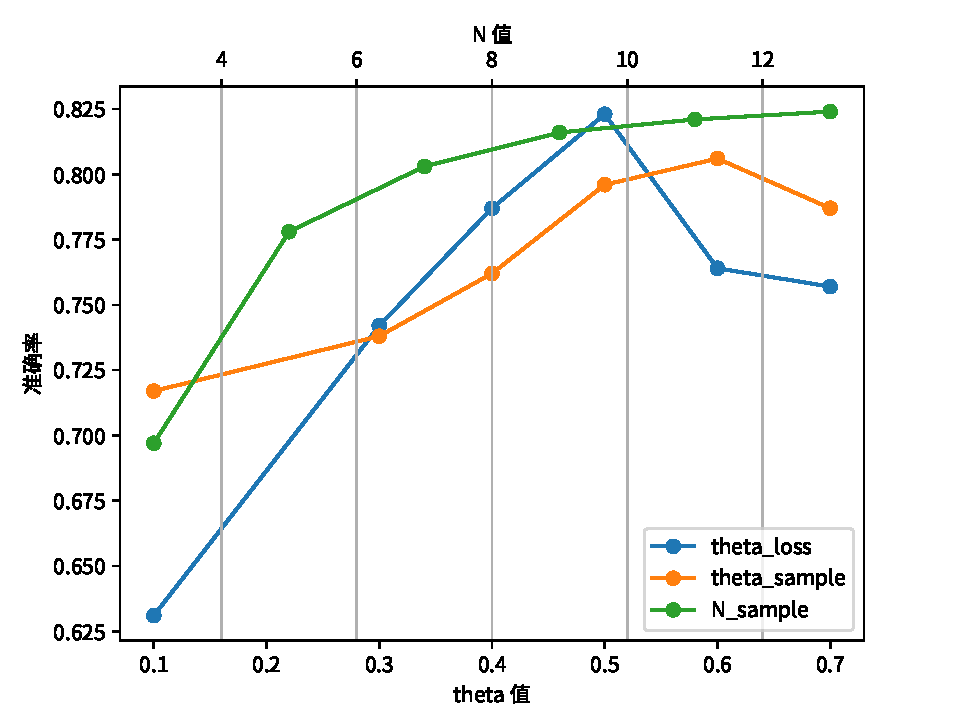
\includegraphics[width=0.9\linewidth]{chapter/c4_images/c4_arg-result.pdf}
    \caption{参数分析实验结果}
    \label{c4_arg-result}
\end{figure}

\subsection{消融实验}

本研究在 GraphSAGE 模型的基础上引入了独特的几种采样、聚合和计算损失的方式,为了验证其有效性,本研究为该模型设置了一组消融实验,该实验将展示这几类引入的算法在何种程度上提升了模型的最终效果。

\subsubsection{实验设置}

在消融实验中,作为对本章所述模型的消融对比,将在 GraphSAGE 模型的基础上替换采样函数、聚合函数和损失函数为各类基线函数,并采用与本章对比实验一致的参数设置,使用同样的数据集进行训练和测试。

实验一共针对模型中的三部分各自设置了三组对照:

\begin{enumerate}
    \item 对于邻居采样方法,设置了完全随机采样和以路径数量采样两种对照方法,对应研究在未引入路径因素和仅考虑路径因素的采样方法的条件下模型的性能变化。
    \item 针对聚合函数,设置了两组在 GraphSAGE 中常用的聚合方法\citing{hamilton2017inductive}作为对照,分别是均值聚合函数和归纳式均值聚合函数。
    \item 对于损失函数,消融实验设置了基于邻居嵌入最小化距离和路径嵌入最小化距离两种对照函数,分别对应于本模型中损失函数的两个极端情况。
\end{enumerate}

\subsubsection{实验结果}

消融实验的结果如表格 \ref{c4_s3tab2} 所示,它反映出了如下的一些特点:

\begin{enumerate}
    \item 本研究引入的基于路径的采样函数、聚合函数和损失函数均在提升异常检测性能上有一定贡献,总的来说,同时引入以上三种方式的模型的提升相比更大,这说明了本章在 GraphSAGE 三个方向提出的方法均在提升异常检测效果上具有作用。
    \item 在损失函数中引入基于路径的因素对模型的影响相比而言更大,一种可能的解释是,损失函数决定了训练参数的目标值,而采样和聚合方法自身在原理具有一定的随机性,从而在模型检测效果上的提升相对较少。
    \item 合理的设置参数 ($\theta$) 能够更好的提升模型异常检测的性能,这是由于在恰当的参数设置下,模型同时引入了路径和图的拓扑上的特征,过大或过小地设定参数将导致单一因素占据决定性比重,从而失去部分特征提取能力。
\end{enumerate}

\begin{table}
    \caption{消融实验结果}
    \begin{tabular}{lcccccc}
        \toprule
                        & \multicolumn{2}{l}{RIPE.2017} & \multicolumn{2}{l}{RIPE.2022} & \multicolumn{2}{l}{DN42.2022}                                                    \\ \cmidrule(lr){2-3} \cmidrule(lr){4-5} \cmidrule(lr){6-7}
        模型              & Acc.                          & F-1                           & Acc.                          & F-1            & Acc.           & F-1            \\ \midrule
        本章所述模型          & \textbf{0.846}                & \textbf{0.837}                & \textbf{0.836}                & \textbf{0.820} & \textbf{0.803} & \textbf{0.794} \\
        \midrule
        邻居采样                                                                                                                                                               \\
        \quad 完全随机采样    & 0.762                         & 0.759                         & 0.774                         & 0.771          & 0.750          & 0.752          \\
        \quad 以路径数量采样   & 0.795                         & 0.783                         & 0.799                         & 0.791          & 0.773          & 0.762          \\
        \midrule
        聚合函数                                                                                                                                                               \\
        \quad 均值聚合函数    & 0.749                         & 0.747                         & 0.752                         & 0.748          & 0.733          & 0.731          \\
        \quad 归纳式均值聚合函数 & 0.745                         & 0.743                         & 0.746                         & 0.744          & 0.730          & 0.735
        \\
        \midrule
        损失函数                                                                                                                                                               \\
        \quad 基于邻居嵌入最小化 & 0.721                         & 0.732                         & 0.725                         & 0.731          & 0.734          & 0.720          \\
        \quad 基于路径嵌入最小化 & 0.793                         & 0.790                         & 0.785                         & 0. 783         & 0.784          & 0.776
        \\
        \bottomrule
    \end{tabular}
    \label{c4_s3tab2}
\end{table}

\section{本章小结}
本章从路由数据的规模出发,研究基于采样和邻居聚合的图网络嵌入方案,并在 GraphSAGE 模型的基础上提出了一套利用数据集的路径属性进行节点嵌入的方法。在 4.1 节,介绍了现有基于图神经网络在大规模图数据上的不足和 GraphSAGE 模型框架在运用于路径式数据上的不足。在 4.2 节,通过对模型进行分析,本文针对 GraphSAGE 模型的三个基本模块进行了探讨,设计出了利用路径特征的对应方法。在 4.3 节,为了验证以上方法在改善原有模型效果上的有效性,进行了对照实验,然后通过消融实验评估了模型在不同设计下的性能。

\chapter{基于随机游走特征嵌入的广域网络路由异常检测研究}

图网络算法在处理基于采样路由的数据集上依然存在丢弃数据集一部分特征的不足,本章从先前几个研究工作的方法和结果上分析提出,将路由数据转换为图网络问题的关键是如何结合依附于路径上的拓扑和属性信息,并将其表示为节点或连边的嵌入。由此思路,可以进一步分析路径自身的统计学含义,从路径的角度出发简化原有问题,进而直接实现路径嵌入的模型构建。由此本章提出了一种基于随机游走特征的嵌入方法,其模型能够准确地捕捉整个数据集中路径的潜在特征。

% 15 页

\section{研究背景}

使用图网络算法进行路由异常检测时,一般的思路是先通过路由数据集中的拓扑信息生成对应的图网络,并将路由上的属性信息标记到节点或连边上,随后通过图网络的嵌入算法获得对应节点或连边的表征。但值得注意的是,在构建图网络的过程中,对于冗余数据的处理方法通常是在预处理阶段就直接丢弃,或者使用一种聚合方法将具有一定意义的属性赋予更高的权重,这样的方式决定了数据集中路径本身的分布状况很容易被忽略,而对于类似网络路由这样的数据集,它的路径集合本身便是通过某种方式采样获得的,其分布具有一定意义。

而基于随机游走的方法,为本研究提供了一种新的思路。随机游走\citing{xie2018efficient}本质上是一种从图网络中进行采样的方法,它能够从采样结果上反映图网络的拓扑结构。对路径的采样能够被理解为对随机数据包路由的跟踪,这使得数据集本身的路径分布情况有了实际意义。

然而,基于随机游走的图算法对采样后的路径分布有要求,而受限于实际采样点的位置、路由会话数量的不一致,这意味着从路由数据集中获取的路由路径并不能直接使用在这些算法上。如何通过巧妙的采样思路还原基于随机游走的路径特征,从而免去数据集处理和初次采样的流程,是一个值得探讨的问题。

为了解决上述挑战,本章节提出了一种不直接依赖现有图模型进行嵌入的方法,即基于随机游走特征的图嵌入方法。该方法首先对问题进行了转换,随后对数据中路由路径的本质做出了假设和具体的数学分析,指出了图网络上的随机游走与广域网上的路由数据存在采样方式上的关联,并提出了一种依靠图网络的权重度量,将路由的拓扑数据二次采样,进而作为后续模型的输入的方法。

% 2 页
综上所述,本章节提出的模型贡献如下:

\begin{enumerate}
    \item 提出了一种检测BGP路由条目异常的框架,充分利用AS Path中的拓扑信息和相关属性,通过基于路径的异常检测更准确地识别和定位异常。
    \item 分析了路由信息的属性,基于BGP的路由特性,提出了一种将网络构造图上的路径转化为加权随机行走路径的方法,并设计了一种在这种约束条件下的数据采样算法,简化并转化了问题。
    \item 设计了一种同时使用拓扑结构和路径属性的方法,以利用数据集中的更多信息,提高检测的稳健性。
\end{enumerate}


\section{问题分析}

% 2 页
% 需要追加

受到 path2vec 模型的随机路径采样方法的启发,对于网络路由的异常检测问题,本章节将以随机游走的角度进行转化和重新阐述,将问题表述为在未知采样规则条件下的路径嵌入问题。

\subsection{问题的定义}

一般而言,在网络的异常路由检测问题上,给定的数据输入为一个网络路由表,即一个或多个路由序列 $R=\{R_1^k, R_2^k, R_3^k, ... R_n^k\}$,其中 $R^k$ 为由包含 $k$ 个不同属性的路由条目。

异常路由检测问题的目标是,在已知部分路由信息 $R_o^k$ 的条件下,通过对路由序列元素的属性进行建模,对新的路由更新信息 $R_{update}^k$ 做出异常检测。

\subsection{问题的转化}

将路由中的 AS Path 信息拆分出来后,以上的路径异常检测问题能够被转化为一个图论问题:

设序列 R 属于一个未知拓扑结构的图 $G<V,E>$,序列 R 是图 G 某种采样规则 $M$ 生成的,序列元素 $R_i<P,C>$ 包含拓扑和属性两个方面的信息,其中,P 的定义为由一系列自治系统编号 $A_i$ 组成的有序列表:$P=\{A_1, A_2, A_3, ... A_m\}$,C 被定义为一个包含标记信息的列表: $C=\{C_1, C_2, C_3,...,C_i\}$。

问题的目标被转化为,在已知部分路由信息 $R_o$ 的条件下,利用其中的 P 对图的拓扑信息进行建模,结合路由信息中的属性值 C,学习一个具有利用二者信息的模型来反应,对新的路由更新信息 $R_{update}$ 做出异常检测。

已知采样规则 M 是通过路由选择算法产生的,即 $R=f_M(G<V,E>)$,最短路径是它采样概率的最重要因素,因此问题的求解可借助某种算法 $f_R$ 去还原路由选择算法的逆变换,即 $f_R = \bar{f_M}$,因此,本文将在后续章节对路由拓扑采样的本质进行分析。

如图 \ref{c5-compare} 所示,本章描述的问题与基于随机游走的图网络嵌入算法(如 node2vec)类似,均通过采样路径获得节点对应的嵌入。与之不同的在于获取采样路径的步骤上:利用图网络度量,能够从原始数据集中采样获得逼近以某种策略为基础的随机游走路径集合,并使用与 node2vec 类似的方式进行图的表征。

\begin{figure}[h]
    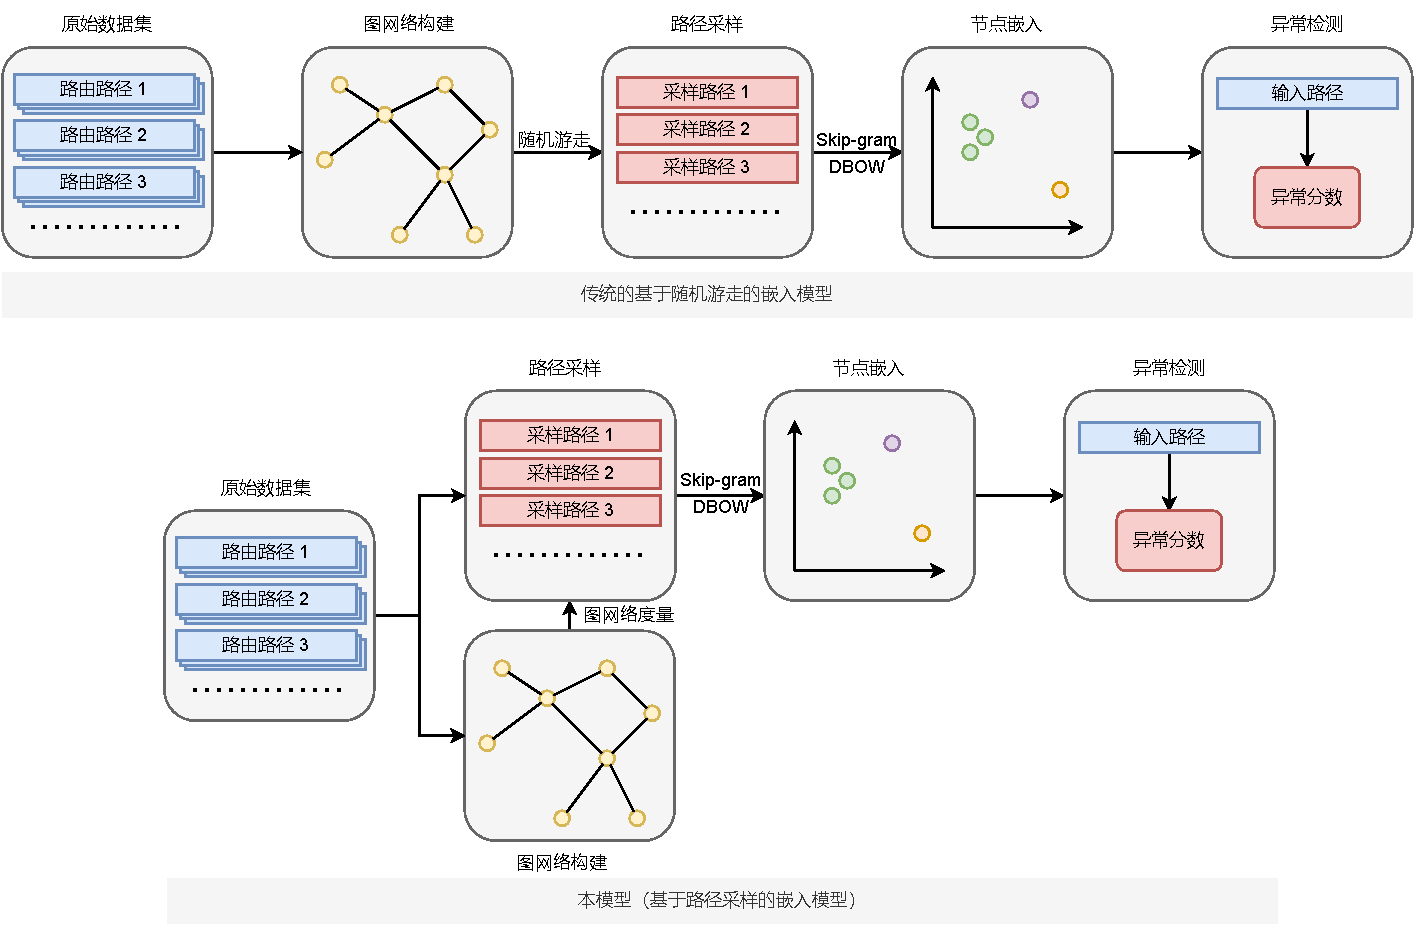
\includegraphics[width=\linewidth]{chapter/c5_images/c5-compare.pdf}
    \caption{基于随机游走的嵌入算法与本章模型的关联}
    \label{c5-compare}
\end{figure}

\section{广域网路由的拓扑分析}

为了能够从分布不一致的图网络数据集中还原出使用基于路由选择算法的采样方式,需要基于数据对广域网的路由拓扑进行分析。在此之前,为了简化问题,本文基于路由协议工作原理,以跟踪数据包在网络中的转发作为随机采样流程,提出以下两个假设:

\subsection{路由属性独立性假设}

该假设认为,路由器对路径和属性上的处理是独立的。即对于一个路由器和其上的路由表 $R$,如何将一个包含特定路由 $R_r$ 的数据包转发到下一跳,将由两个独立的过程完成:

\begin{enumerate}
    \item 根据 $P_r \in R_r$ 决定转发路径,进而决定转发优先级。
    \item 根据 $C_r \in R_r$ 决定路由代价,进而决定转发优先级。
\end{enumerate}

在以追踪数据包的转发的方式构建随机游走路径的情况下,任意相邻节点的转移概率将由两个独立过程决定,基于这一前提,路由数据中的路径 $P_r$ 和社区属性 $C_r$ 即可被拆分为两组独立数据交由两种不同的模型处理。

\subsection{稳定采样规则假设}

该假设认为采样规则 $M$ 是稳定的。对于一个链路状况不断变化的网络而言,自治系统之间的连接状况常常发生改变,这一现象体现为图上边集 $E$ 的改变,从而带来了拓扑结构和路径属性上的改变,在随着时间改变的动态图结构上进行采样将引入复杂的时间因素,并大幅提高模型的维度和参数量。因此,本研究需要针对网络路由数据集的采样特点,总结其在时间方向的变化特征。

广域网络常常由数万乃至百万台网络设备组成,为了保证自治系统在其路由策略上的一致性,通常而言路由优先级的选择不会在短时间(例如路由异常的时间段内)产生突变,在节点数 $n(V)$ 和边数 $n(E)$ 足够大的网状网络中,链路之间的冗余是常见的,这等效为采样规则在一定范围内是稳定的,即 $M(t_1) = M(t_2)$。因此,路由选择算法的确定性保证了路由数据集在局部采样规则上是相对稳定的。


\section{模型设计及实现}

% 5 页

在这一节,本文将对 BGP 路由中的异常检测问题的本质进行探讨,并对其做出公式化的推理,通过一种新颖的方式将其转化为另一种基于随机游走的路径的问题。为了验证上述思路的正确性,本研究还据此实现了一种多步异常检测模型,它的基本结构如图 \ref{c5-model} 所示,主要由采样、嵌入、聚合和异常检测部分组成。

\begin{figure}[h]
    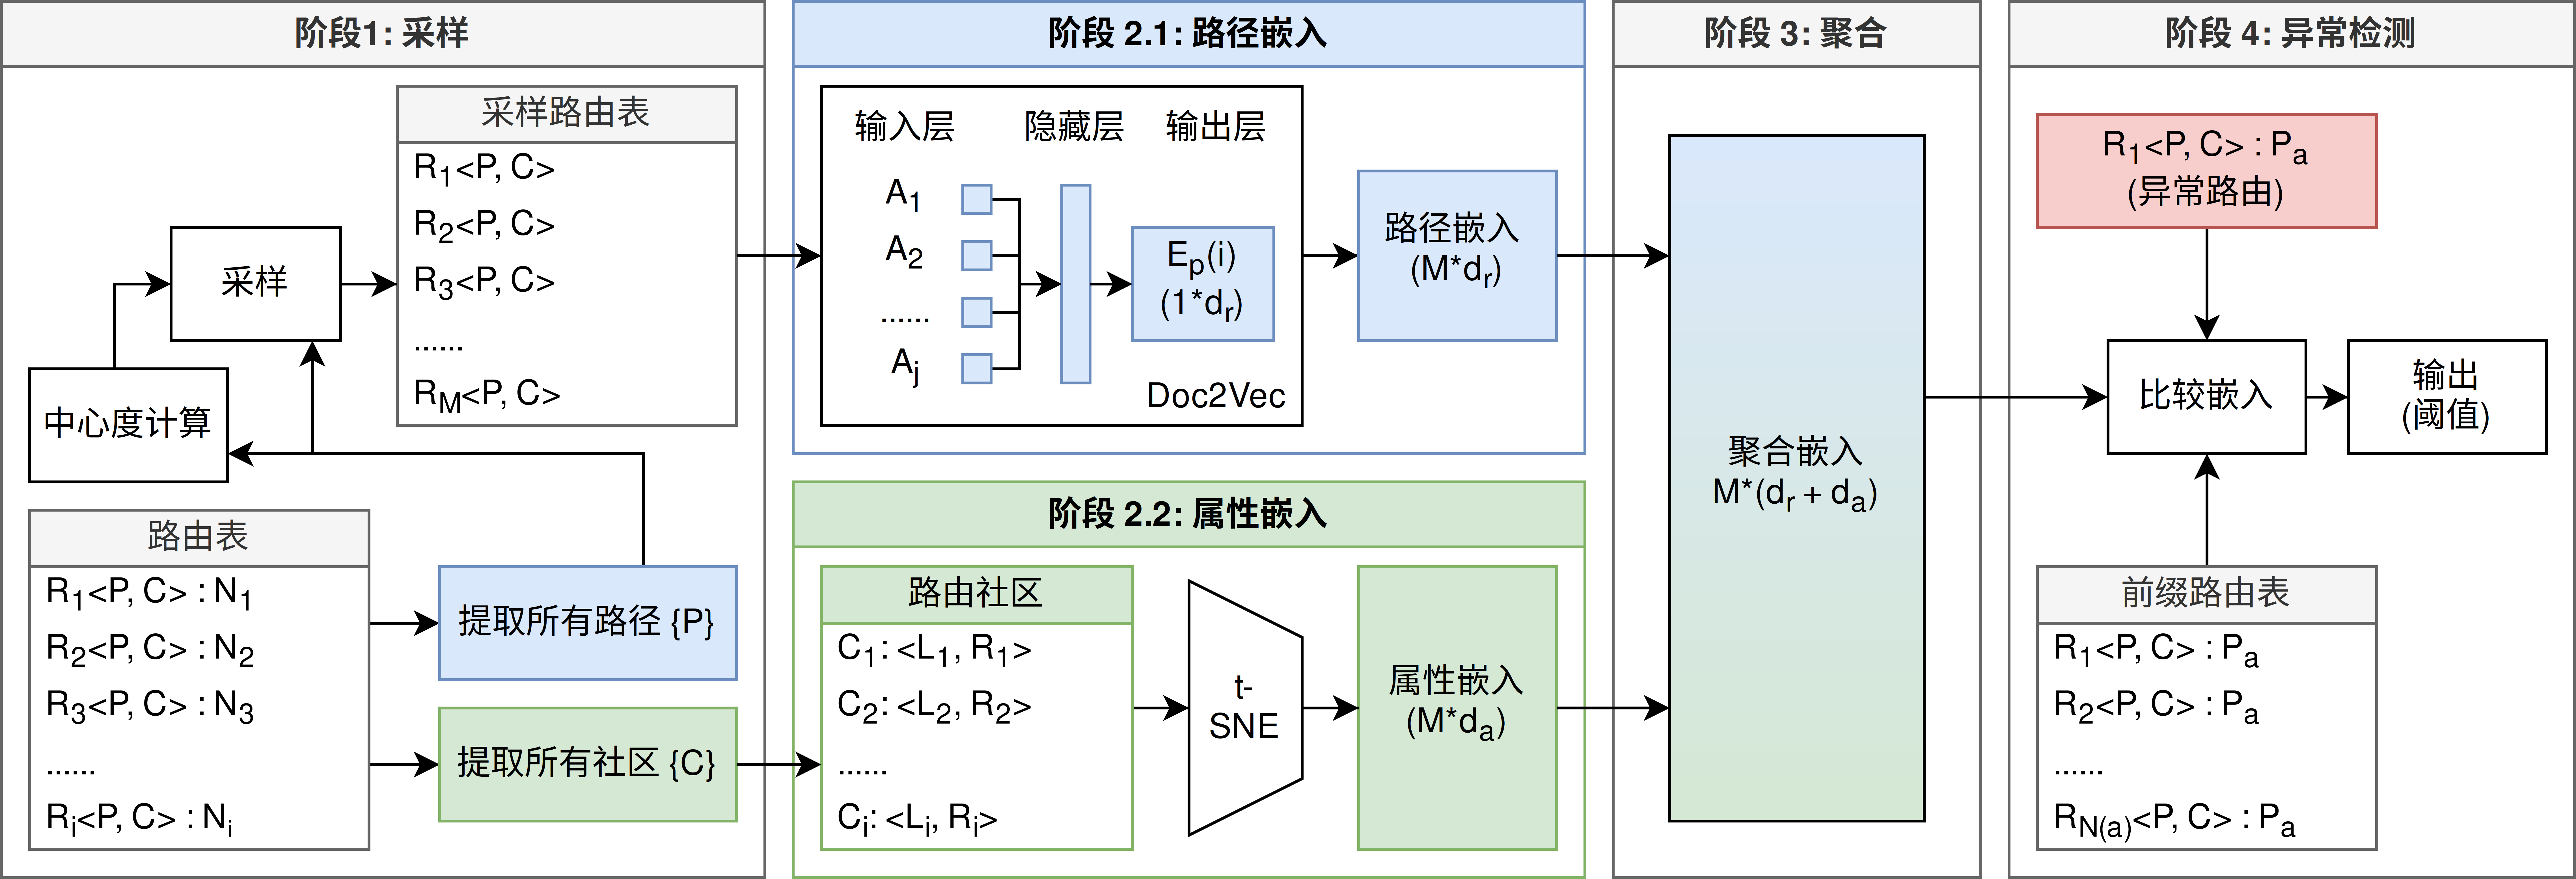
\includegraphics[width=\linewidth]{chapter/c5_images/c5_model.png}
    \caption{模型结构图}
    \label{c5-model}
\end{figure}

\begin{enumerate}
    \item 采样模块反映了本节研究的核心观点,使用了一种新颖的方式采样路由路径,并分离其中的拓扑和属性特征。
    \item 路径嵌入模块对采样后的、符合随机游走的统计学特征的路径集进行学习并获得对应的嵌入向量。
    \item 属性嵌入模块则是根据路由的社区属性,对其进行降维处理,获得社区属性对应的嵌入向量。
    \item 聚合模块将二者结合起来,作为最终的嵌入信息。
    \item 异常检测模块使用基于嵌入误差的方法对路由更新进行相似度计算,给出异常检测分数结果,并可选地根据阈值判断路由异常。
\end{enumerate}

\subsection{基于路由度量信息的样本采样}

这是模型的第一部分,它利用了随机游走的思想,将数据视作为随机游走的等效结果,通过一种等效化采样的方法处理原始数据,使其分布满足一种特定的基于最短路权重的随机游走采样方法,以便于后续通过基于随机游走的图网络嵌入进行异常检测任务。

\subsubsection{图上的随机游走}

本步骤的核心观点在于,将路由数据集中的路由条目的自治系统路径属性与在图上进行随机游走后产生的路径相关联起来。为了实现并验证这一目标,需要对网络拓扑上的数据集采集方法的特点进行分析。

边界路由协议在一般情况下,对路由选择的影响反映在自治系统路径和社区属性上\citing{feamster2004model},它们共同作用决定某个网络将以何种路径被抵达。由于不同运营商的社区属性定义一般是不一样的,此类信息仅能作为一种拓扑无关的特征使用,本文在随机游走性质的研究主要体现在自治系统路径,即拓扑信息上。

在路由表中宣告的每一个地址块 B 都对应着至少一个可访问的网络,以及至少一条路由条目 $\{R_1, R_2, ... R_n\}$。根据本章前一节的分析,路由表$\{B_1,...B_m\}$中的每个地址块所涉及到的路由则可以理解为一种随机游走策略:以数据包的视角而言,随机游走路径实质上是从随机的采集点$\{A\in{A_1, A_2...}\}$出发,经过 $m \times n$ 轮采样到达地址块源网络的路径集合。

因为它是一种有效的随机游走采样方法,只要输入的数据满足这样的条件,就可以对路由进行进一步的嵌入,进而进行异常检测。

\subsubsection{基于随机游走介数中心度的路径采样}

由于广域网络的路由选择模型是通过最短路径实现的,对这样的数据构图更适合介数中心度指标。然而,实际的路由数据集中的数据并不是最短路径,不同的自治系统和基于 BGP Add-Path (RFC5492)\citing{walton2016advertisement}的路由收集会话都会发送同一网络的不同前缀的次优路由,在此场景下,传统的介数中心度指标会受到此类因素的干扰,与实际拓扑对应的值存在偏差,因此基于随机路径的数据需要一种新的度量方式。由于上述原因,为了更好地度量在非最优路径集合内,某一节点对网络的影响力,本研究引入了随机游走介数中心度这一度量单位。

如公式\ref{betweeness}所示,通常情况下的介数中心度被定义为一个节点作为两个其他节点之间最短路径上的桥梁的次数。
\begin{equation} \label{betweeness}
C_{betweenness}(v) = \Sigma_{s \neq v \neq t \in V}\frac{\sigma_{st}(v)}{\sigma_{st}}
\end{equation}
根据此公式,对于图中的每一对顶点 $s,t \in V$,计算它们之间的最短路径$\sigma_{st}$,随后对每一个顶点计算通过该顶点的最短路径$\sigma_{st}(v)$的加权和。

而数据集中的路由显然不满足这一条件,它包含不同位置、不同网络、不同发送策略的路由,因而将使用“不那么最短路径”的度量来衡量它的介数中心度。

由于 BGP 路由在一般情况下遵循最短自治系统路径原则,并且大部分 BGP 劫持都是通过宣告更短自治系统路径的路由进行的,路由表中的路由条目中的路径部分 $P$ 显然在一定程度上是通过在真实的网络拓扑 $G \left\langle V,E \right\rangle$ 下使用某种基于随机游走的介数中心度的方法进行采样的结果路径集合。

Newman 提出了一种对随机游走进行中心度度量的方法,它被称为随机游走介数中心度。\citing{agryzkov2014new} \citing{newman2005measure} 该度量单位以公式\ref{rw_betweeness}的方式被定义。
\begin{equation} \label{rw_betweeness}
C_{RWbetweenness}(v) = \Sigma_{s \neq v \neq t \in V}\ p_{st}(v)
\end{equation}
该公式去除了最短路径的条件,从而计算路径集合内每一条可行的路径中,经过点$v$路径的加权和,在本研究中,连通$s,t$路径的全集即为路由数据集中以$s,t$分别作为起始和结束节点的自治系统路径。

有了上述前提,问题的目标现在被转化为,在已知部分路由信息 $R_o$ 的条件下,进行二次采样 $M‘$,使得采样的结果与在 G<V,E> 上进行加权随机游走 $M_r$ 的结果一致,即 $M_r(G<V,E>) = M'(M(G<V,E>)) = M'(R_o)$ ,对新的路由更新信息 $R_update$ 做出异常检测。

模型需要先根据给定路径 $R_o$ 计算出各个节点的随机游走介数中心度,并据此采样出 $m'(R_o) \in R_o$。

值得注意的是,网络路由数据集大多是由配置了路由反馈会话的路由器向收集器发送全部或者部分路由,并不遵循以随机游走介数中心度为权重进行随机游走的采样规则,因此需要使用以下的采样方法来使处理后的数据集达到期望的分布。

此处规定等价采样 $M'$ 的输入是包含若干网络 $\{N1,N2,...N_{N_{prefix}}\}$ 的路由表,$M'$ 将对输入中的每个 N 中的路由项 R 进行采样,使得 $j < i$。

具体来讲,对于每一个网络路由 $N_i$,模型对其包含的路由的路径子集 $\{P_1, P_2, P_3, ... P_{n_{route}(i)}\}, R_i<P_i, C_i> \in N_i $ 进行随机游走介数中心度的计算,得到一个节点与中心度的映射 $A_i \rightarrow C_{RWbetweenness}(A_i)$,随后以公式\ref{omega_p}规定路径的采样权重为它路径上的平均中心度:
\begin{equation} \label{omega_p}
\omega_p(P_i) = \frac{\sum_{A_i \in P_i}^{len(P_i)} C_{RWbetweenness}(A_i) + \theta}{len(P_i)}
\end{equation}

最终的采样结果使用 $R_{sampled} = top(k, R_o)$,$\theta$ 在这里起到了控制路径长度的作用,当 $\theta \gg \sum C_{RWbetweenness}(A_i) $ 时,可以近似的认为是完全以路径长度作为度量进行采样。

\subsection{路由路径与特征嵌入}

\subsubsection{基于 Doc2Vec 的路由拓扑嵌入}

在这一阶段,模型将以路径作为模块的输入,使用模型捕获路径中的拓扑关系,输出对应的嵌入。本文将先从 Node2Vec 出发探讨这一可能性,随后介绍本模型实际使用的 Doc2Vec 方法\citing{le2014distributed}。

对于传统的随机游走嵌入模型,通常的方法是使用 Node2Vec 来从采样后的路径中获得节点的嵌入\citing{grover2016node2vec},然而,由于 Node2Vec 仅能够对单个节点进行表征,无法对路径及其属性进行建模,因此需要将其进行拓展。

Doc2Vec 是一种从可变长序列(通常是文字)中提取嵌入特征的方法\citing{le2014distributed},它能够通过提取序列间元素的关系,直接对整个序列生成特征向量。

正如节点 V 能够与词语表征相对应,采样路径 P 也能够与段落表征相对应,这与 node2vec 和 word2vec 的对应关系类似。通过基于 Doc2Vec 的 path2vec 模型,能够更好地捕获路径中节点间的关联,即路由每一跳之间的联系,将采样路径转换为嵌入向量。

Doc2Vec 模型存在两种不同的训练方法,分别称为 DM(Distributed Memory)和 DBOW(Distributed bag of words)\citing{murdock2014learning}。对于本文所涉及到的问题而言,Distributed Memory 方式获得的向量能够作为输入序列的上下文,因而更适合在此场景中使用。

因此,本文将路径列表使用 Distributed Memory 方法放入 Doc2Vec 模型中进行训练,然后对每个路径输出一个 $d_r$ 长度的向量作为路径的表征。

\begin{figure}[h]
    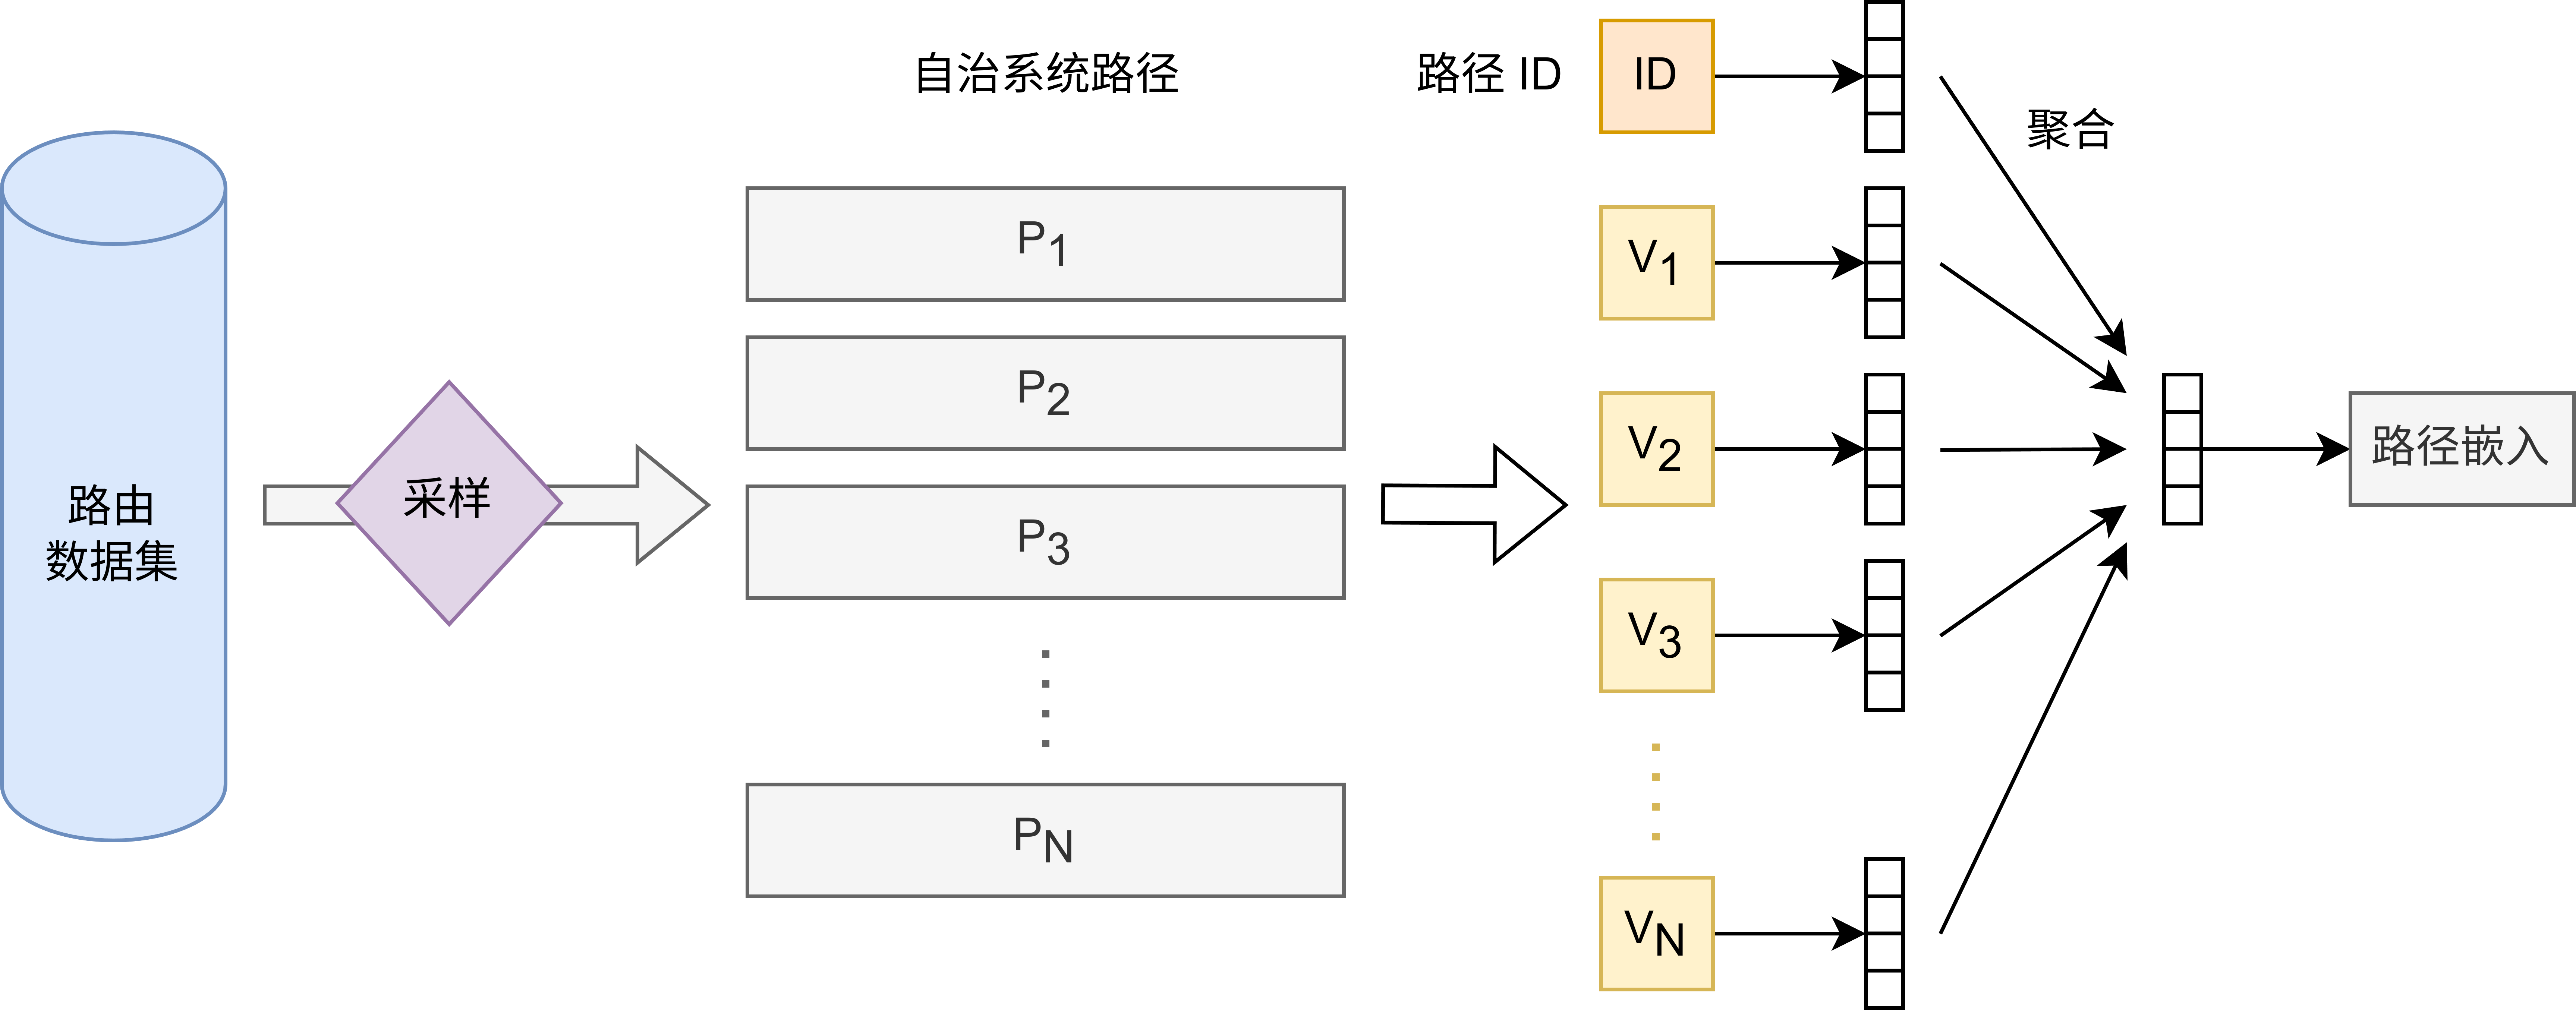
\includegraphics[width=0.9\linewidth]{chapter/c5_images/c5_model-dm.png}
    \caption{使用 Distributed Memory 方法训练路径嵌入}
    \label{c5_model-dm}
\end{figure}

% 图

如图 \ref{c5_model-dm} 所示,在模型中,每一个路径都被赋予一个唯一的 ID,并将其映射到矩阵 D 的其中一列以表示上下文信息,在此之后,路径中的每一个节点都将被映射到矩阵 W 中的其中一列,它们共同被输入 Doc2Vec 模型中,通过 Distributed Memory 方法转换为一列嵌入向量,从而被用于下游的异常检测任务。

\subsubsection{基于 t-SNE 的路由属性嵌入}

在路径拓扑进行嵌入之外,另一个模块是对路径的属性进行嵌入表示,由于 Community 属性并不包含特定的拓扑信息,在不同网路中定义方式也差异很大,模型在这里直接将 Community 映射到一个特定的 one-hot 向量,然后通过 t-SNE 对数据进行降维\citing{van2008visualizing},将其输出为 $d_a$ 长度的向量作为特征的表征。

\subsection{特征的聚合和异常检测}

由于前面两个模块分别输出路径的拓扑和属性两个方面的嵌入,这一模块目的是将其结合起来作为最终的嵌入向量用作后续的异常检测。

对于异常检测而言,只需对新的路由 $R_{update}$ 进行一次嵌入计算,然后将其与现有的对应路由 $R_{exist} \in R$ 进行相似度对比,偏移过大的路由条目将作为异常路由输出。

具体的相似度计算使用如公式\ref{s5_cos_dist}所述的余弦相似度方法:
\begin{equation} \label{s5_cos_dist}
D_{cos}(A,B) = 1 - \frac{\sum_{i=1}^{d_r+d_a} A_i B_i}{\sqrt{\sum_{i=1}^{d_r+d_a} A_i^2}\sqrt{\sum_{i=1}^{d_r+d_a} B_i^2}}
\end{equation}

\section{实验分析}

% 5 页

为了验证和展示本文所提出的模型的有效性和准确性,本文将在这一节设计几个实验,并且根据任务的目标获取与之对应的数据集,从不同规模和结构的数据集上对模型进行评估,随后对模型进行消融实验和参数分析,以确定模型的各步骤的有效性,最后通过真实网络环境下的路由劫持对模型进行案例分析。

\subsection{数据集设置}

由于模型要求输入未经修改的路由路径,本章节的实验将根据具体需求使用来自互联网(RIPE RIS) 和 DN42 两种分布式网路的数据,这两类数据集在数据规模、复杂度和结构特点上有所不同,在先前章节的表 \ref{dataset-compare} 展示了数据集的基本统计信息,对于本章的模型而言,其中最重要的信息为数据集内路由路径的数量和长度,这决定了它们将要学习的特征的数量和复杂度。

对于异常检测而言,本文提出的模型是无监督的,它将会给出所有符合异常条件的路由。同时,由于模型的输出结果是基于给定的阈值的二值化,而阈值在很多情况下依赖于检测策略并且在精确度和召回率之间做出权衡,因此本文在实验阶段的部分分析中将去掉这一步,从而使用以下方式计算模型的准确度:

在案例分析的实验中,本研究将会在历史数据中选取一些众所周知的 BGP 劫持或异常事件作为实验数据集,同时,实验还将利用 DN42 网路的实验性特点,在线地在实际网络中运行测试,并将其实时状态作为案例分析的实验数据集。

\subsection{对比实验}

在该实验中,本文将该方法与3类具有代表性的基线模型进行了比较,它们包括如下几种参考模型:

\begin{enumerate}
    \item 基于图数据的方法。作为代表的有 DeepWalk 和 GraphSAGE,前者与本模型采用相同的采样并从路径中学习嵌入的思路,而后者则是基于图卷积网络优化的邻居聚合算法。
    \item 基于路由属性的方法。该方法通常使用一般路由属性进行异常的判断,而不借助图网络结构,本章实验采用了一种基于专家知识定义的决策树的方法\citing{li2005internet}作为传统方式的对比。
    \item 基于时间序列的方法。本实验采用了一种基于小波变换(Wavelet)的方法\citing{mai2008detecting}和一种基于 LSTM 的方法\citing{cheng2016ms}作为对比。
\end{enumerate}

\subsubsection{参数设置}

本实验从 RIPE RIS 中调取了三个著名的 BGP 事件期间的 MRT 路由数据集以便获取有标注的异常路由序列,它们分别发生于 2010、2017 和 2022 年,并同时调取了存在标注的 2022 年的 DN42 MRT 路由数据集。为了在实验中取得相同的度量单位,实验按照事件时间跨度的 200\%,等比例地划分了 128 份路由更新数据,将其与事件发生前的路由表快照信息一同放入模型中,实验使用异常发生前 1 天的路由数据作为无异常路由的训练输入。对于本模型的参数选择,$\theta$ 被设置为接近互联网自治系统平均距离的一般数值,即 $\theta=3$,作为对照的模型各选择其推荐的对应参数。

\subsubsection{实验结果}

\begin{table}
    \caption{对比实验结果}
    \begin{tabular}{lcccccccc}
        \toprule
                        & \multicolumn{2}{l}{2010AS23724} & \multicolumn{2}{l}{2017AS39523} & \multicolumn{2}{l}{2022AS14618} & \multicolumn{2}{l}{DN42.2022}                                                                     \\ \cmidrule(lr){2-3} \cmidrule(lr){4-5} \cmidrule(lr){6-7} \cmidrule(lr){8-9}
        模型              & Acc.                            & F-1                             & Acc.                            & F-1                           & Acc.           & F-1            & Acc.           & F-1            \\ \midrule
        基于图数据                                                                                                                                                                                                                     \\
        \quad DeepWalk  & 0.768                           & 0.770                           & 0.754                           & 0.741                         & 0.750          & 0.757          & 0.751          & 0.755          \\
        \quad GraphSAGE & 0.793                           & 0.820                           & 0.815                           & 0.808                         & 0.784          & 0.814          & 0.807          & 0.801          \\
        \midrule
        基于路由属性                                                                                                                                                                                                                    \\
        \quad 决策树(专家规则) & 0.824                           & 0.815                           & 0.793                           & 0.772                         & 0.727          & 0.718          & 0.736          & 0.729          \\
        \midrule
        基于时间序列                                                                                                                                                                                                                    \\
        \quad Wavelet   & 0.845                           & 0.831                           & 0.839                           & 0.820                         & 0.837          & 0.833          & 0.814          & 0.796          \\
        \quad LSTM      & 0.844                           & 0.841                           & 0.858                           & 0.834                         & 0.815          & 0.813          & 0.825          & 0.833          \\
        \midrule
        此模型             & \textbf{0.887}                  & \textbf{0.879}                  & \textbf{0.894}                  & \textbf{0.891}                & \textbf{0.902} & \textbf{0.897} & \textbf{0.875} & \textbf{0.870} \\
        \bottomrule
    \end{tabular}
    \label{c5_s2tab}
\end{table}

该实验采用了异常检测的准确度和F-1值的方法来评估模型异常检测的性能,以下表格反映了本异常检测模型在处理此类事件上获得的准确性表现。从此模型的表现中得到以下发现:

\begin{enumerate}
    \item 本章所述模型在不同时间段和不同规模(互联网路由数据集规模是逐年增长的)的事件上都取得了较好的效果。尤其在 2022 年的 RIPE RIS 数据上取得了 90\% 以上的准确度,考虑到一半的互联网络数据集在未被标记为异常状况时自身也存在少量路由拓扑的改变和更新,从而具有一定程度的背景干扰,该模型环比其它模型在准确性上的提升较大。
    \item 在先前章节的实验中,值得注意的一点是对于类似于 DN42 的分布式网络数据集而言,模型的性能相比互联网数据集将有所降低。而在此实验中能够观察到模型在 DN42 数据集上的性能损失并不明显,这说明了模型在不同类型网络的数据集,尤其是小规模数据集上具有良好的泛化特性。
    \item 传统的基于专家知识和时间序列特征的模型在新的互联网数据集和其它分布式网络数据集上面临大幅度的性能下降,这是由于此类数据集随着时间的变化,一些与异常检测模型相关的关键特征也随之发生变化,从而无法将原有的模型在未更改结构的情况下使用在新的数据上。
\end{enumerate}

\subsection{消融实验}

本研究引入了一种独特的路径采样函数,为了验证其基于随机游走的介数中心度的采样方法的正确性,需要为模型设置一组独特的消融实验,该实验将展示参数 $\theta$,即采样比重是如何通过改变随机游走规则所占比重从而影响节点的表征的。

\subsubsection{实验设置}

消融实验将模型中的路径采样函数进行了修改和替换以供对照,本实验中采用了一般中心度、路径长度、随机选择的三种方式作为对比,它们分别以如式\ref{compare_eq1}、\ref{compare_eq2}、\ref{compare_eq3}的方式被定义。
\begin{equation} \label{compare_eq1}
\omega_{centrality}(P_i) = \frac{\sum_{A_i \in P_i}^{len(P_i)} C_{betweenness}(A_i) + \theta}{len(P_i)}
\end{equation}
\begin{equation} \label{compare_eq2}
\omega_{length} =  \frac{\theta}{len(P_i)}
\end{equation}
\begin{equation} \label{compare_eq3}
\omega_{averaged}(P_i) = const
\end{equation}

随后,本文在与对比实验中相同的数据集上进行实验,除修改的采样参数外其它各参数设置和测试指标保持不变。

\subsubsection{实验结果}

运行消融实验,结果如表格 \ref{c5_s3tab} 所示,能够通过该实验得到如下结论:

\begin{enumerate}
    \item 在采用了基于本章所述的结合路径长度与随机游走介数中心度的采样方法的条件下,模型的各项异常检测结果均优于其它用于对照的模型,这证明了上述采样方法的有效性。
    \item 随机选取的采样方式(即平均化采样概率)下,模型等效于直接将原始路径输入到路径嵌入模块中,较差的异常检测结果反映出了原始数据集在采样路径分布上的不均衡,从而较大的影响了模型的性能。
    \item 基于中心度的方式对数据集路径进行采样的最终效果总体上优于基于路径长度的方式进行采样,这说明了路由数据集中主要的路径特征更倾向于遵循中心度度量的方式分布。
\end{enumerate}

\begin{table}
    \caption{消融实验结果}
    \begin{tabular}{lcccccccc}
        \toprule                      & \multicolumn{2}{l}{2010AS23724} & \multicolumn{2}{l}{2017AS39523} & \multicolumn{2}{l}{2022AS14618} & \multicolumn{2}{l}{DN42.2022}                                                                     \\ \cmidrule(lr){2-3} \cmidrule(lr){4-5} \cmidrule(lr){6-7} \cmidrule(lr){8-9}
        模型                            & Acc.                            & F-1                             & Acc.                            & F-1                           & Acc.           & F-1            & Acc.           & F-1            \\ \midrule
        本章所述模型                        & \textbf{0.887}                  & \textbf{0.879}                  & \textbf{0.894}                  & \textbf{0.891}                & \textbf{0.902} & \textbf{0.897} & \textbf{0.875} & \textbf{0.870} \\
        一般中心度 ($\omega_{centrality}$) & 0.840                           & 0.827                           & 0.837                           & 0.834                         & 0.855          & 0.838          & 0.826          & 0.819          \\
        路径长度 ($\omega_{length}$)      & 0.818                           & 0.814                           & 0.811                           & 0.810                         & 0.835          & 0.829          & 0.817          & 0.802          \\
        随机选择 ($\omega_{averaged}$)    & 0.796                           & 0.791                           & 0.803                           & 0.799                         & 0.790          & 0.786          & 0.781          & 0.775          \\
        \bottomrule
    \end{tabular}
    \label{c5_s3tab}
\end{table}

\subsection{参数分析}

为了分析采样参数 $\theta$ 在控制策略进而影响模型检测效果上存在怎样的工作原理,本文设置了一组实验用于分析 $\theta$ 在不同取值下的模型效果。

\subsubsection{实验设置}

实验选取了上述对比实验中的 RIPE RIS 数据集,在其余参数保持不变的情况下使用 $\theta = 1$ 和 $\theta = 3$ 分别对正常路由更新/异常路由更新进行异常检测,并将其正则化的异常分数进行统计。

\subsubsection{实验结果}

如图 \ref{c5_arg-analysis},从实验结果中可以看出,设置一定长度的 $\theta$ ,即采样比重,能够在整体上改善模型的检测效果,本实验将其设置为互联网中的自治系统平均距离的大约一半,为 3.00。一种可能的原因是采样比重 $\theta$ 限定了自治系统路径的长度,从而通过采样筛除了一些不常见的路由项,从而提高了准确性。

此外,图 \ref{c5_arg-analysis} 中也能够反映出,即使是在被确认并不存在大规模的异常路由更新的数据集上,模型依然会对一小部分路由更新输出较高的异常检测分数,一种合理的解释是,互联网络本质上是一种随时改变拓扑结构的图网络,因此除了能够大范围或较大程度地改变异常路由的事件外,还会频繁地出现小规模的局部拓扑更新,这部分更新反映在异常检测上即是一种背景噪声。这类小范围的路由更新不会在广域网络中长时间持续传播,因此并不会在异常检测分数上对结果产生决定性的干扰。

\begin{figure}[h]
    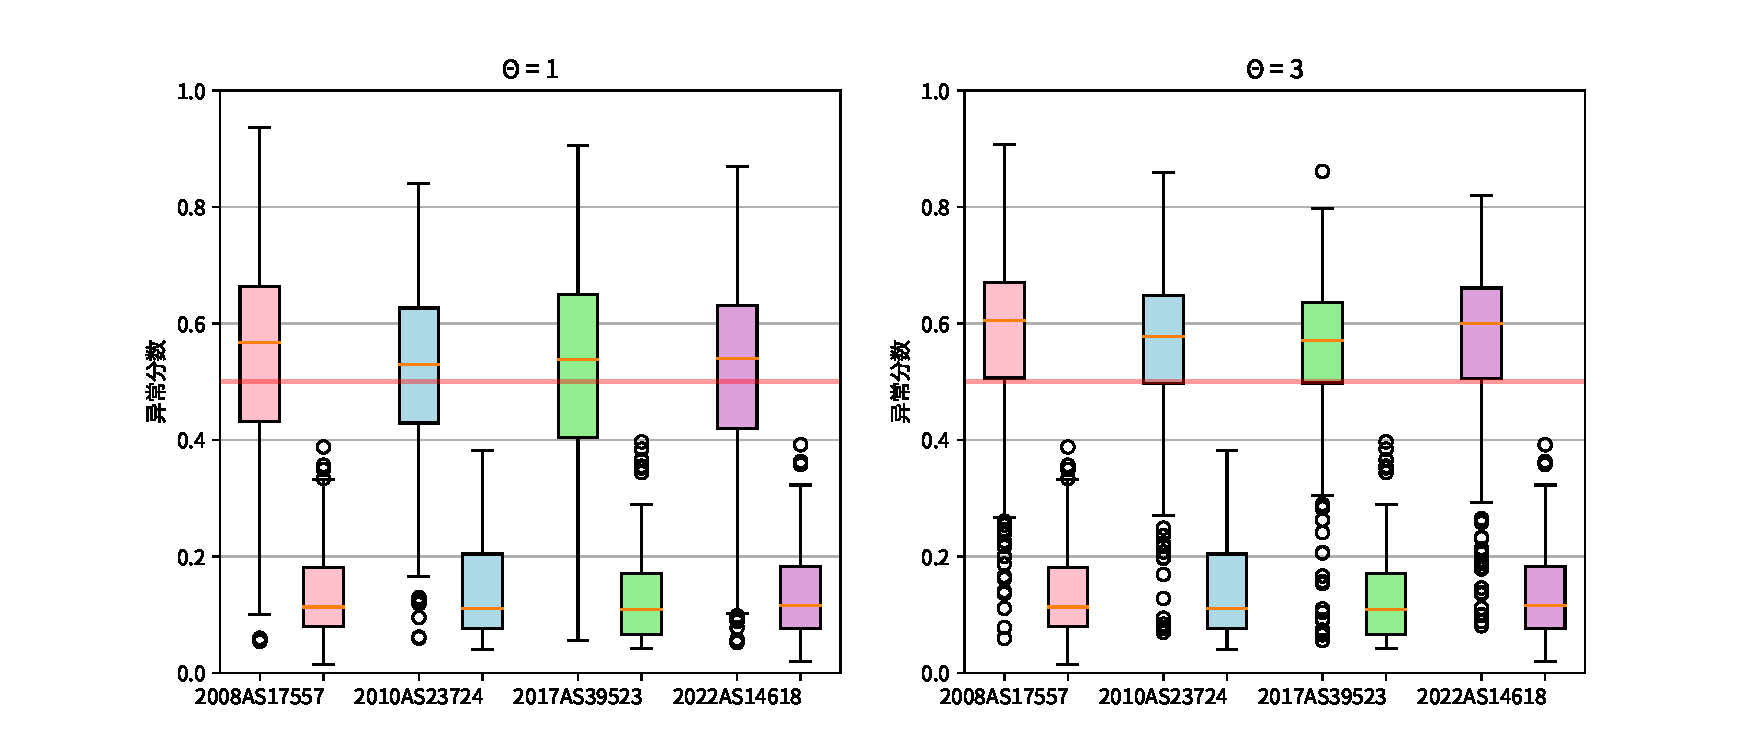
\includegraphics[width=\linewidth]{chapter/c5_images/c5_arg-analysis.pdf}
    \caption{参数分析结果}
    \label{c5_arg-analysis}
\end{figure}

% 对于 RIPE RIS 上的已知案例,通过调整参数确定参数与效果的关联。

\subsection{案例分析}

由于历史上具有标记、全球性的路由异常事件非常稀少,仅通过对已有路由异常的重放来测试模型的识别能力并不足够。因此,本文还设置了一组案例分析实验用于模拟真实的路由劫持事件,并由此分析模型在面对不同网络环境下路由异常的性能。

\subsubsection{实验设置}

本文在先前章节中提及了 DN42 的基本概况,它是一个社区构成的实验性网络,具有灵活的组网方式和具有相对较少限制的社区规范,这使得本实验能够实际生成具有劫持效果的 BGP 路由,并通过路由收集器(即 DN42 GRC)获取包含异常路由的数据集。

在此实验的预备工作中,本研究首先以自治系统 AS4242421332 的身份接入到 DN42 网络中,并将两个 IP 前缀通过 BGP 协议向 DN42 其它自治系统进行了宣告。在维持正常的网络路由一段时间后,正常的路由表能够被路由收集器收集并生成数据集文件,其中即包含了以该自治系统为起点到达网络中一部分自治系统的最优和次优路径集合。

随后,进行实验的异常路由部分,本实验在另一个能够控制的自治系统 AS4242421331 中以路径改写的方式,宣告一系列具有劫持效果的路由,意图将通往目标网络的流量劫持至该网络。此行为将被网络自身及其各阶邻居通告给路由收集器,随后以更新文件的形式将包含异常路由的路由表 MRT 文件生成出来。

异常检测模型将以这两个文件作为输入,输出对流量劫持开始后的 BGP 路由更新的异常检测分数。同样的,此实验按照 200\% 时间跨度,等比例地划分了 128 份路由更新数据。

\subsubsection{实验结果}

在获得了正确的异常检测输出后,本实验将路由嵌入的平均余弦距离与时间的关系以图表的方式输出,以便于分析模型检测路由异常后的输出是否稳定和合理。

\begin{figure}[h]
    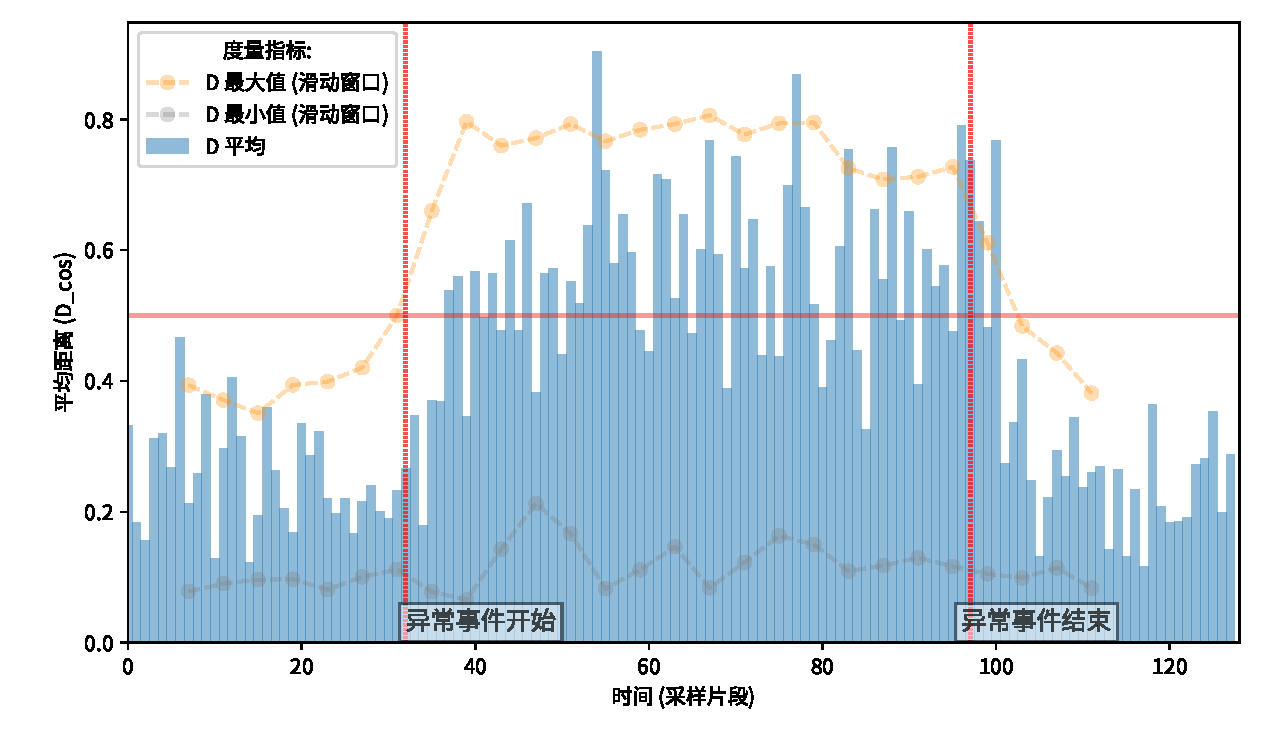
\includegraphics[width=\linewidth]{chapter/c5_images/c5_route-distance.pdf}
    \caption{时间序列上的特征距离分析}
    \label{c5_route-distance}
\end{figure}

如图 \ref{c5_route-distance} 显示,如使用 top-k 在一段时间分析路由异常的最大值或者平均值,模型是能够明确判断出路由异常的,以最大特征距离为标志的度量值在劫持发生后立即升高并突破 0.5 的阈值。此外,通过对比不同的指标可以观察到,特征距离最小值在整个事件中没有明显变化,一种可能的原因是 BGP 路由的更新在广域网络的邻居间相互传递,收敛较为缓慢,部分网络中存在的路由震荡抑制机制也使得突发的 BGP 更新无法及时反映到 GRC 的数据中,由于同样的原因,对于平均路由距离值而言,它相比异常的发生存在一定的延后时间。

通过 t-SNE 对异常发生前后的更新路径与原路径的表征进行降维,能够以此作出路径嵌入的可视化预览图,以分析此段时间内路由嵌入的状况,如图 \ref{c5_case-study-scatter},可见更新的路由被映射到了一个远离正常路径的区域(图中的红色区域)。值得注意的是,即使在未被标记为异常的时间段内的路由数据中,依然存在与异常数据较为接近或与其它路由更新距离较远的路由嵌入,这部分路由被认为是网络中偶发的拓扑改变所产生的背景噪声(图中的黄色区域是其中的一部分示例),这与参数分析中的图 \label{c5_arg-analysis} 的结果相对应。

\begin{figure}[h]
    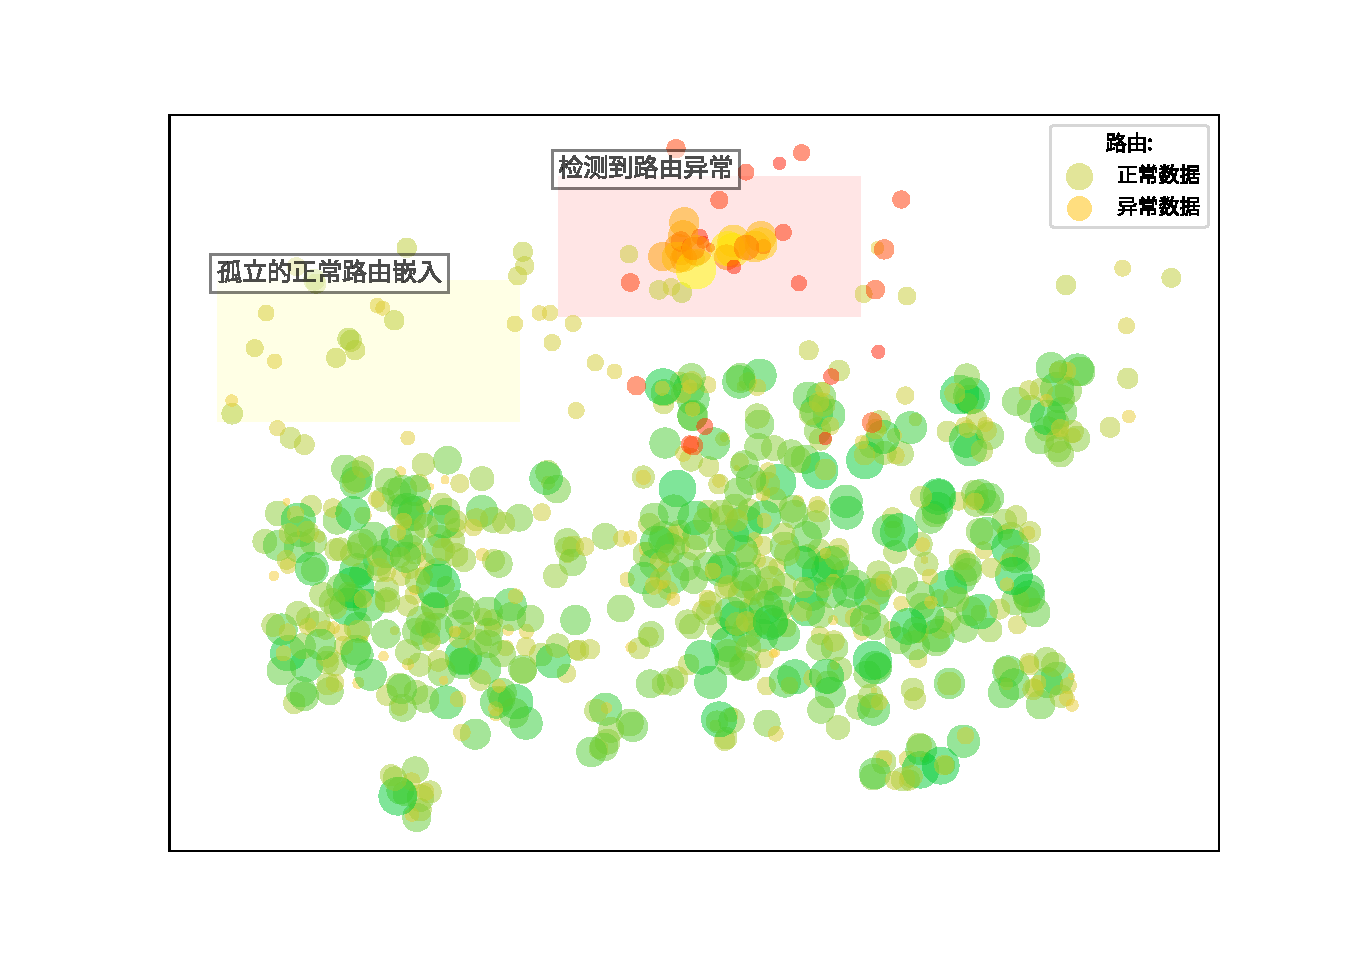
\includegraphics[width=\linewidth]{chapter/c5_images/c5_case-study-scatter.pdf}
    \caption{异常发生后的更新路径与原路径的表征}
    \label{c5_case-study-scatter}
\end{figure}


\section{本章小结}

本章尝试从数据集的路径采样特征入手,提出了一种基于随机游走中心度的采样方法,并构造了利用路由路径拓扑和属性直接获得路径嵌入的模型。在 5.1 节,简述了基于构图的图网络模型在路径特征上存在利用不足的问题。本文在 5.2 节分析了路由异常检测问题的本质,并将其转化为一种采样问题。在 5.3 节,承接上述问题,提出了基于两个假设的实证分析,确定了使用基于最短路径和随机游走模型为主的采样方法来解决路径特征问题。在 5.4 节,提出了具体的采样方法,并将其与一个完整的异常检测模型配合,概述了模型的结构。本文在 5.5 节通过对比实验、消融实验和案例分析等方法验证了该模型的性能,并验证了路径采样方法的效果。

\chapter{全文总结与展望}

% 2 页 1500 字

\section{全文总结}

% 1.5 页
广域网络中的路由异常,因为其隐蔽、复杂和无法根除的特点,成为了近年来通信和计算机领域中一个值得深入研究的问题。大多现已提出的算法和应用于工业中的模型还尚在使用基于时间序列分析的方式研究此问题,而选择此种研究方式意味着放弃数据集中的几乎全部拓扑信息,使得学习到的模型在泛化性上存在不足,很难使用于各种分布式网络中。因此本文立足于网络路由系统的图网络本质,通过对网络数据的嵌入建模的方式来实现对路由异常的预测。本文从三种角度研究了对网络路由数据的建模方法。首先,本文从数据的角度出发,探讨了现有网络数据集存在的不足,提出了一种新的网络数据集构建算法。随后,本文研究了基于 GraphSAGE 算法的聚合模型,针对数据特点提出一种新的聚合函数和损失函数。最后,本文在随机游走的基础上分析了路由路径的特点,提出了一种对路由数据进行针对性采样的检测模型。

首先,为解决现有数据集在图网络上存在冗余数据过多、无效边集影响模型效果、并非针对图网络算法等问题,本文构建出了一套用于将常规网络路由数据集构建为图网络的构图算法。具体而言,该算法从网络的逻辑拓扑出发,利用网络自身的路径选择算法的特点,提出了一种去除冗余和无效链路的方法,从而降低图的复杂性;此外,还从节点的相似性角度出发,使用一种基于相似度的图网络构造方法生成数据集。使用两种不同的图网络生成算法在不同的典型基线模型上进行了多方面的实验,进一步验证了该方法提升了原有数据集在图网络下的性能。

其次,为了解决传统基于图卷积网络模型难以处理庞大网络数据的问题,本文提出了一种基于属性信息聚合的异常检测模型。通过对 GraphSAGE 模型在邻居采样过程的分析,本论文提出了一种基于邻接节点路径聚合的聚合函数模型,这种模型能够有效地利用节点的邻接节点信息和与之相关联的路径信息,相对应地,本文还提出了一种适用于路径特征的损失函数。几种基线模型对特定路由异常进行评估的结果显示该模型在一些场景下能够更好的预测异常,同时通过消融实验验证聚合函数和损失函数模型在异常检测性能上有更好的表现。

最后,本文直接从数据集的路由采样的随机游走特征出发,提出一种利用节点的拓扑信息对路由数据集本身进行采样的方法。然后在此基础上设计了一个新颖的异常检测模型,同时使用采样路径和路由本身的社区属性进行基于路径的表征,此模型降低了问题的复杂性,摆脱了以路径为单元的异常检测任务对完整构图的依赖。本文针对此模型设计了在多种路由数据集上的预测实验,并针对路径采样模型设置了消融实验,结果显示模型在有效性上优于各基线模型,然后从实际网络运行状况的角度设置了案例分析,验证了模型在真实应用场景下的可靠性。

\section{后续工作展望}
% 0.5 页

针对本文进行的三个方向上的研究尝试,后续工作的研究方向可以总结为如下内容:

\begin{enumerate}
    \item 在针对路由数据的图网络构建模型方面,本文采用的基于对等边集的建模方式是对路由数据在图网络结构下的朴素分解方式,它依赖与一些与网络连接性相关的参数设置,从而缺少在不同数据集上的泛用性。如何结合节点的邻域特点,更好地找出图网络中的层次拓扑结构,将会是下一步工作值得尝试的主题。
    \item 对于基于信息聚合的图异常检测模型而言,本文提出的邻居聚合算法和损失函数通过节点在路径中的位置选择权重,而没有考虑到节点自身包含的属性也能够作为计算权重的依据之一,下一步工作可尝试通过节点的属性表征对邻域的聚合算法做出改进,例如在邻居聚合步骤引入注意力机制。
    \item 在基于随机游走特征嵌入的算法模型上,由于本文提出的采样模型是依赖完整构建的图网络参数的,它依然需要涉及到对大型网络拓扑进行计算,没有在模型中彻底去除对预先构建网络的依赖,下一步的研究可面向如何进一步降低计算复杂度,从而使得模型能够处理更大的数据集。
\end{enumerate}



% misc

\thesisacknowledgement

三年时光转瞬即逝,无数个昼夜的学习与研究终化作这数十页论文,而我自己也将告别若干年朴素的学生时代,向自己未知的命运出发。

毕业在即,感慨万千。此时我愿将最真挚的感谢献给我的导师--邵俊明教授,不仅是因为他严谨的学术态度和一如既往地对我的研究的帮助和指导,更是因为他一直以来对学生和教研室的关心体现出了独特的人格魅力。毫无疑问,在我的项目、研究和论文中,都离不开邵俊明教授的关注、审阅和指导,他在专业和人生上都将是我最崇敬的老师。

同窗三年,我要将最真诚的祝愿和感谢送给教研室的小伙伴们,科研之路充满坎坷,相互扶持才让我们前行至此。他们对我的帮助、鼓励和包容,让我能够在这三年中,直面学习、科研和生活等多方面的挑战。祝愿他们能够拥有美好而光明的前程。

同时,我还需要感谢陪伴了我四年的学生组织 NetUnion,它为我提供了绝佳的学习氛围和环境和实践自己想法的空间,一同工作的同事们思想开放、技术高超、学术拔尖、善良包容,令人终身难忘。

最后,需要感谢某位小可爱一直以来的陪伴,生活不易,数不清多少个夜晚我潸然泪下,最终又紧紧相拥。即将因毕业而分隔两地,惟愿我们终获幸福的未来。

我以此文作为人生之分隔符,标志着一段人生历程画上句号,及另一段新的旅程的开始。祈愿从此自由地在阳光下起舞。

% \input{misc/appendix}

% Uncomment to list all the entries of the database.
%\nocite{*}

\thesisbibliography{reference}

%
% Uncomment the following code to load bibliography database with native
% \bibliography command.
%
% \nocite{*}
% \bibliographystyle{thesis-uestc}
% \bibliography{reference}
%

\thesisaccomplish{publications}
% \input{misc/translate_original}
% \input{misc/translate_chinese}

\end{document}
